\documentclass[11pt,a4paper,oneside]{memoir}
%\documentclass[11pt,a4paper,twosides]{memoir}
%\documentclass[11pt,a4paper,openany]{book}

%%%%%%%%%%%%%%%%%%%%%%%
% set pagesytle
%%%%%%%%%%%%%%%%%%%%%%%

\setstocksize{11in}{8.5in}
\settrimmedsize{\stockheight}{\stockwidth}{*}
\settrims{0in}{0in}
\settypeblocksize{9.0in}{5.75in}{*}
%\setlrmargins{1.25in}{*}{*}
\setlrmargins{*}{*}{1.5}
\setulmargins{1.2in}{*}{0.5}
\setheadfoot{16pt}{30pt}
\setheaderspaces{0.7in}{*}{*}
\checkandfixthelayout

%%%%%%%%%%%%%%%%%%%%%%%
% set chaptersytle
%%%%%%%%%%%%%%%%%%%%%%%

\usepackage[svgnames]{xcolor}
\usepackage{fix-cm}
\definecolor{numbercolor}{gray}{0.7}
\newif\ifchapternonum
\makechapterstyle{jenor}{
  \renewcommand\printchaptername{}
  \renewcommand\printchapternum{}
  \renewcommand\printchapternonum{\chapternonumtrue}
  \renewcommand\chapnumfont{\fontfamily{pbk}\fontseries{m}\fontshape{n}%
    \fontsize{1in}{0in}\selectfont\color{numbercolor}}
  \renewcommand\printchaptertitle[1]{%
    \noindent%
    \ifchapternonum%
    \begin{tabularx}{\textwidth}{X}%
    {\parbox[b]{\linewidth}{\chaptitlefont ##1}%
      \vphantom{\raisebox{-15pt}{\chapnumfont 1}}}
    \end{tabularx}%
    \else
    \begin{tabularx}{\textwidth}{Xl}
    {\parbox[b]{\linewidth}{\chaptitlefont ##1}}
    & \raisebox{-15pt}{\chapnumfont \thechapter}%
    \end{tabularx}%
    \fi
    \par\vskip2mm\hrule
  }
}
\chapterstyle{jenor}
%\chapterstyle{ell}

%%%%%%%%%%%%%%%%%%%%%%%
% packages
%%%%%%%%%%%%%%%%%%%%%%%

\usepackage{
  calc,
  url,
  fancyvrb,
  multicol,
  indentfirst,
  ulem,
  wrapfig,
  kvsetkeys
}
\usepackage[yyyymmdd]{datetime}
\usepackage{tikz}
\usepackage{graphicx}
\usepackage[columns=2]{idxlayout}
\usepackage{kotex}
%\SetHangulFonts{hkbt}{wgt}{uttz}
\ifpdf
\usepackage[colorlinks]{hyperref}
\hypersetup{
  linkcolor=blue
}
\fi

%%%%%%%%%%%%%%%%%%%
% titlepage setup
%%%%%%%%%%%%%%%%%%%

%%% for the Fontsite 500 fonts
\newcommand*{\FSfont}[1]{%
  \fontencoding{T1}\fontfamily{#1}\selectfont}
%\renewcommand*{\FSfont}[1]{}%    kills special font selections
\newlength{\drop}

\newcommand*{\titlePP}{\begingroup% Printing Poetry
%\FSfont{5jr}% FontSite Jenson Recut (Centaur)
\drop=0.06\textheight
\vspace*{\drop}
\begin{raggedleft}
%{\HUGE\color{Navy} PUZZLING}\\[\baselineskip]
{\HUGE\color{MidnightBlue} 천문학과 대학원생을 위한}\\[\baselineskip]
{{\LARGE{대학원 입학, 생활, 연구}}}\\[1.1\baselineskip]
{\HUGE\color{MidnightBlue} 매뉴얼} \\[\baselineskip]
{\Large by 천문학과 대학원생 일동}\par
\end{raggedleft}
\vfill
\begin{center}
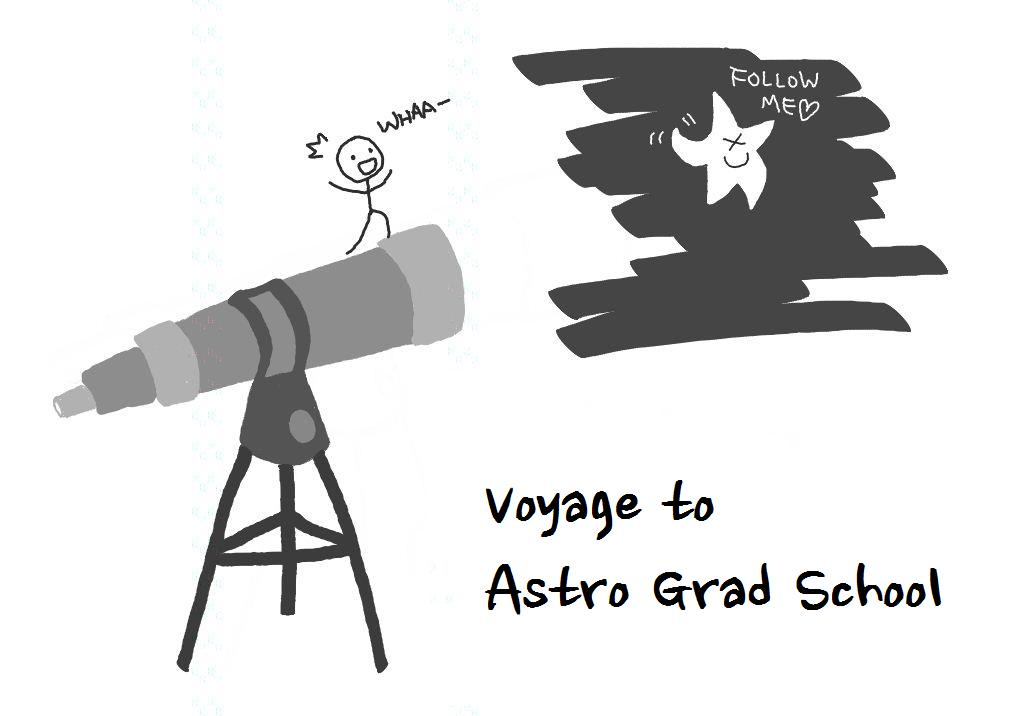
\includegraphics[width=6in]{./Figures/cover_mod.jpg}
%{\normalfont\fontsize{192pt}{192pt}\selectfont ?!}
\end{center}
\vfill
\begin{center}
{\large \textsc{Ver 1.1}}
\end{center}
\vspace*{\drop}
%\mbox{}
\endgroup}


%%%%%%%%%%%%%%%%%%%
% indexpage setup
%%%%%%%%%%%%%%%%%%%
\renewcommand*{\indexname}{찾아보기}
\usepackage{makeidx}
\makepagestyle{index}
  \makeheadrule{index}{\textwidth}{\normalrulethickness}
  \makeevenhead{index}{\rightmark}{}{\leftmark}
  \makeoddhead{index}{\rightmark}{}{\leftmark}
  \makeevenfoot{index}{\thepage}{}{}
  \makeoddfoot{index}{}{}{\thepage}
\makeindex

%%%%%%%%%%%%%%%%%%%%%%%%%%%%%%%%%%%%%%
% commands, environments, etc.
%%%%%%%%%%%%%%%%%%%%%%%%%%%%%%%%%%%%%%

\setlength{\parskip}{0.2\baselineskip}
%\newcommand\starbreak{\fancybreak{\decosix\quad\decosix\quad\decosix}}
\newcommand\starbreak{\fancybreak{$*\quad*\quad*$}}
\renewcommand*{\bibname}{참고문헌}
\renewcommand*{\contentsname}{차례}
%%% Use footnote symbol
\renewcommand{\thefootnote}{\fnsymbol{footnote}}

\newenvironment{packed_enum}{
\begin{enumerate}
  \setlength{\itemsep}{1pt}
  \setlength{\parskip}{0pt}
  \setlength{\parsep}{0pt}
}{\end{enumerate}}
\newenvironment{packed_item}{
\begin{itemize}
  \setlength{\itemsep}{1pt}
  \setlength{\parskip}{0pt}
  \setlength{\parsep}{0pt}
}{\end{itemize}}

%%% ToC down to subsections
\settocdepth{subsection}
%%% Numbering down to subsections as well
\setsecnumdepth{subsection}

%%%%%%%%%%%%%%%%%%%%%%%%%%%%%%%%%%%%%%%%%%%%%%%%%%%%%%%%%%%%%%%%%%%%%%
%%%%%%%%%%%%%%%%%%%%%%%%%%%%%%%%%%%%%%%%%%%%%%%%%%%%%%%%%%%%%%%%%%%%%%

\begin{document}

\begin{frontmatter}
\OnehalfSpacing
\pagestyle{empty}
\titlePP

\clearpage
% copyright page
\begingroup
\footnotesize
\setlength{\parindent}{0pt}
\setlength{\parskip}{\baselineskip}
%%\ttfamily
\textcopyright{} 2014 --- 서울대학교 천문학과 대학원 \\
All rights reserved

Astronomy Program, Seoul National University, Seoul.

이 책의 PDF 버전과 소스 파일들은 서울대학교 천문학과 대학원생
홈페이지(\url{http://astro.snu.ac.kr/~grad})에서 찾아볼 수 있습니다.

\begin{center}
\begin{tabular}{ll}
  Ver 1.0 : \hspace{2cm}   & 2012년 3월 \\
  Ver 1.1 : \hspace{2cm}   & 2014년 1월 \\
% Second impression, with corrections:    & 2 July 2001 \\
\end{tabular}
\end{center}
최종 수정일: \today
% \fi

\endgroup
\clearpage

\tableofcontents
\clearpage

\chapter{추천사 - 아프니까 대학원생이다.}

나는 대학원생이다. 
이 얼마나 설레는 말인가. 
꿈과 열정과 이성으로 넘치는 젊음으로 대학원 생활을 누리는 사람들! \\

그러나 하루하루 밤낮을 가리지 않고 좌충우돌하면서 맨 땅에 헤딩을 하다보면 몸과 마음이 아파진다. 안개 속에서 나아갈 길이 보이지 않는 때도 가끔씩 있다. 아프니까 대학원생이다. 그래도 신난다.\\

패러다임이 변하고 있다. 맨 땅에 헤딩하다보니 개천에 용들이 사라졌다. 이제는 맨 땅에 헤딩하기 전에 헬멧을 써야 한다. 여기 손 주비 군을 비롯한 헌신적인 대학원생들이 모여 대학원생용 헬멧을 준비했다. 이 헬멧을 쓰면 마음껏 좌충우돌하며 어려움을 헤쳐 나갈 수 있을 것이다. 이 헬멧은 완전하지는 않지만 헬멧으로서의 역할을 충분히 할 것이다. 연구를 통해 헬멧은 계속 개선될 것이다.\\

날아라, 대학원생들이여.\\
전 세계에서 자랑스럽게 높이 나는 흑룡이 되기 바란다.   

{\raggedleft{\scshape 이명균} \\ 2012년 3월 13일\par}

\chapter{여는말}
천문학과 대학원 생활 안내서를 펼친 여러분을 환영한다.

 이 길고 긴 안내서는 서울대학교 천문학과 대학원 신입생들이 대학원에 입학하여, 지도 교수님을 선정하는 과정부터 시작해서 대학원 생활에 적응하는 법, 수료와 졸업을 위한 여러 가지 절차들, 그 외에 연구에 도움이 되는 다양한 팁들을 총 망라한 문서이다. 많은 대학원 신입생들이 느낄 법한, 대학원에 첫 발을 내디뎠을 때의 막막한 시간을 최소화하고, 빠르게 적응할 수 있도록 도움을 주기 위해 작성되었다. 뿐만 아니라, 기존 대학원생들의 연구와 대학원 생활에 관한 다양한 정보를 공유하고, 하나의 문서에 모아 기록에 남기기 위함도 있다. 

 이 안내서에 담긴 내용들은 서울대학교 천문학과 대학원생들이 직접 느끼고, 경험한 것들을 바탕으로 한 다양한 노하우를 담고 있다. 그러나 한편으로는 공식적인 문서는 아니기 때문에, 이를 잘 활용하기 위해서는 각자가 필요한 부분을 차근히 읽어보되, 각종 공문서, 행정실, 대학 본부, 지도 교수님 등을 통해 확인하는 과정을 거칠 것을 추천한다. 

 이 안내서는 크게 네 부분으로 이루어져있다. 첫 번째 부분은 ‘대학원 생활 시작’에 관한 것으로 지도 교수 선정 과정부터 각 연구팀 소개, 컴퓨터 세팅, 강의 소개, 그 외에 기타 생활 적응에 관한 내용을 다루고 있다. 두 번째는 ‘대학원 생활’과 관련한 부분이다. 천문학과 대학원에서 있을 다양한 행사들과, 그 구성원으로서 대학원생들의 역할 등에 대해 소개한다. 세 번째 부분은 실제 연구에 관련한 내용들을 담고 있다. 천문학 관련 논문과 서적에 대한 소개 및 이를 정리 및 활용하는 방법들을 소개한다. 또한 실질적으로 천문학 연구에 활용되는 다양한 프로그램들에 대한 간략한 소개와 유용한 팁 들을 공유하고자 한다. 또 천문학회에 대해서, 자신의 연구를 효과적으로 발표하는 요령, 천문학 (특히 관측 천문학)에서 중요한 관측 제안서 작성 등 천문학 연구 방법에 대한 폭넓지만 얕은 소개도 적어놓았다. 마지막 장에서는 졸업에 관련하여 논문 제출 자격 시험 준비와 졸업 논문 주제 제안, 학위 심사를 준비하는 과정들을 설명하고 있다.

 서울대학교 천문학과는 대학원은 소수의 구성원이 가족과 같은 관계를 구축하고 있으며, 하늘과 우주에 대한 열정을 공유하는 훈훈한 분위기를 자랑한다. 처음에 발을 내딛는 신입생들에게는 조금 낯선 분위기일 수 있으나, 적응하고 나면 그 정을 함빡 느끼면서 연구할 수 있는 낙원(?)과 같은 곳이다. 천문학에 대한 열정과 호기심을 해결하는데, 이만한 곳도 없을 것이다. 그러니! 처음엔 조금 적응이 어려워도, 기존 구성원들과 소통해가며 차근히 적응해보자. 그리고 그 적응과 열정 가득한 연구 생활에 이 안내서가 작은 빛줄기가 되기를 기원한다. 여러분의 연구 여정에 성공만이 가득하길 기원한다. Bon Voyage~!

{\raggedleft{\scshape 저자 일동} \\ 2012년 3월\par}




\end{frontmatter}
\clearpage

\begin{mainmatter}
\OnehalfSpacing
\chapter{대학원 생활 시작하기}
\epigraph{바트! 대학원생 놀리지 말거라.\\그냥 잘못된 선택을 한 것 뿐이야.}
{\textit{$\langle$The Simpsons$\rangle$,\\ \textsc{Marge Simpson}}}
% Tikz Reference: http://www.texample.net/tikz/examples/transparent-png-overlay/
\begin{tikzpicture}[remember picture, overlay]
    \node[inner sep=0pt] at (1.in,0.9in) {%
        
\includegraphics[width=2.4in]{./Figures/bart.jpg}%
    };%
\end{tikzpicture}
\begin{tikzpicture}[remember picture, overlay, opacity=0.8]
    \node[inner sep=0pt] at (2.7in,1.08in) {%
        
\includegraphics[width=1.2in]{./Figures/marge.jpg}};%
%    \draw[red,ultra thick,rounded corners] (2.in,1.28in) rectangle (1.2in,2in);
\end{tikzpicture}

\section{지도 교수 선정 및 팀 소개}
모 선배님 왈.. 지도 교수님을 선정하는 것은 배우자를 선택하는 것만큼이나
중요하다!! 매일 얼굴을 보고 학위 과정 중 매우 중요한 연구에 대해 이야기를 나누며
졸업 후에도 연구 내외적으로 관계가 평생 유지되기 때문이다. 이와 같이 매우 중요한
지도교수님을 선정하게 되는 과정에 대해 얘기를 해보자.

기존의 지도 교수 선정은 입학하자마자 ‘난 이 교수님을 택하겠어!’라는 다짐(?)과
함께 행정실 조교님께 메일을 보내고, 교수 회의를 통해 결정되면 끝나는 매우 단순한
과정이었다. 하지만 대학원 신입생들이 어떤 교수님이 어떤 연구를 하시는지 자세히 알
수 없어 이 과정이 부적절하다는 결론이 내려졌다. 그래서 2012년 2학기
신입생들부터는 지도 교수 선정 과정이 한 학기 뒤로 미루어졌다. 신입생들은 입학
직후에 해당학기 학과장 교수님을 지도 교수님으로 하여, 첫 학기에는 개별 지도
교수님 없이 수업을 듣게 된다. 대학원 생활 첫 학기에는 신입생 세미나인 ‘현대
천문학 특강’이라는 과목을 듣게 되는데, 이 과목에서는 매주 다른 교수님들이
들어오셔서 각 교수님의 현재 연구 주제 등에 대해서 알려주신다. 이러한 신입생
세미나 과목을 들으면서 자신의 관심 분야와 일치하는 교수님이 어떤 분인지를 생각해
보고, 학기가 끝날 때 쯤 행정실 조교님이 보내주시는 지도 교수 선정 관련 메일에
답장을 드리면 된다. 물론 이 수업을 통해 교수님들의 연구에 대해 많은 것을 알 수
있지만 연구실 분위기나 교수님의 스타일 등에 대해서 알기는 쉽지 않으므로 각
연구팀의 선배들에게 질문을 하고 조언을 구하는 것도 아주 좋은, 혹은 굉장히 필요한
방법이라고 할 수 있겠다. \\

자, 그렇다면, 서울대학교 천문학과의 각 연구팀에 대해 알아보자.

\subsubsection{구본철 교수님 팀}
\begin{figure}
\begin{center}
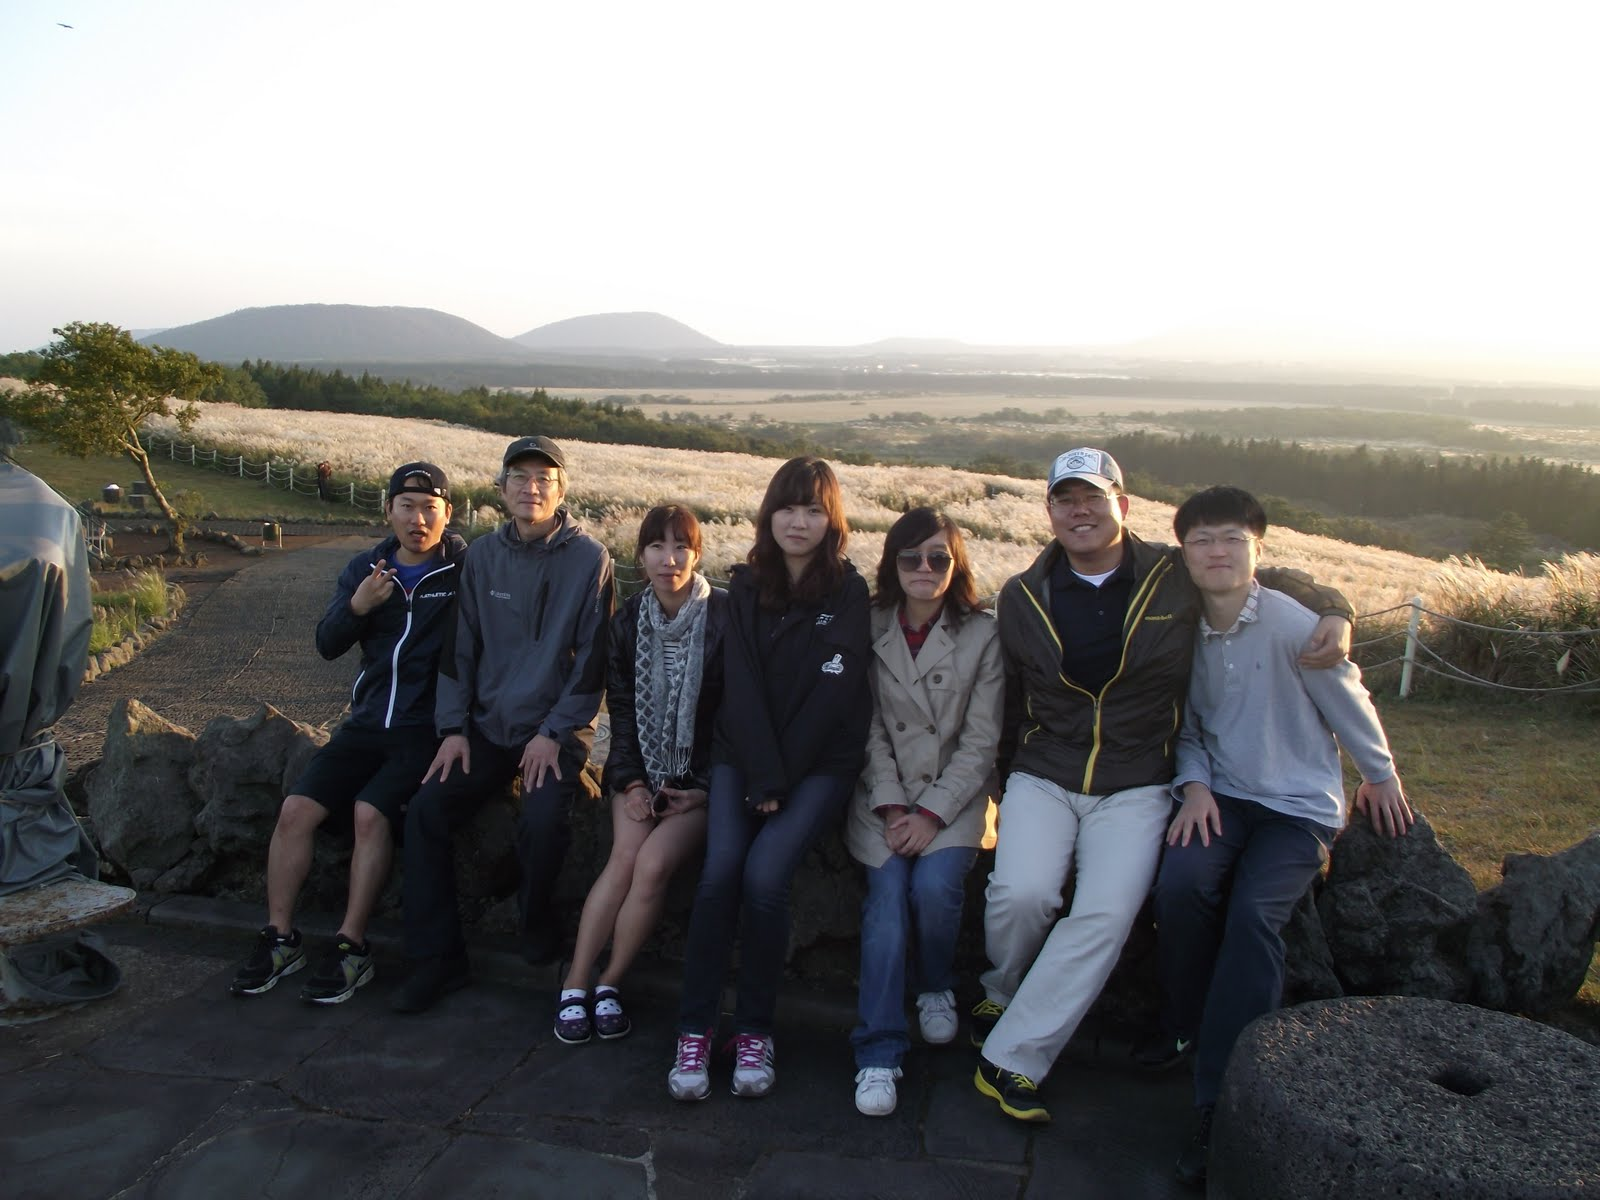
\includegraphics[width=0.85\textwidth]{./Figures/team-koo.jpg}
\legend{\textsf{구본철 교수님 팀---2011년 가을 제주도에서}}
\end{center}
\end{figure}
구본철 교수님 예하 팀 구성원들은 다양한 관측 자료를 이용하여 작게는 별의 탄생과 죽음에서부터 크게는 우리은하 내 성간물질의 구조와 진화에 이르는 광범위한 분야에 대해 관심을 가지고 다음과 같이 폭넓은 연구를 진행해 오고 있습니다.
\begin{packed_enum}
\item 우주망원경인 AKARI, Herschel, Spitzer 와 지상망원경인 AAT, Palomar, UKIRT 등으로부터 확보한 적외선 이미징 및 분광 자료를 활용한 별 탄생지역과 초신성잔해 연구. 
\item I-GALFA 서베이 자료와 SRAO 의 전파 관측 자료를 이용한 우리은하 중성수소의 구조 및 초신성잔해와 CO 분자운과의 상호작용에 대한 연구. 
\item 초신성 잔해의 진화, 성간난류 및 별 생성 등에 대해 수치 계산을 통한 이론연구
\end{packed_enum}
이러한 연구들은 한국천문연구원(KASI), 일본 우주항공연구개발기구(JAXA), 아레시보 전파관측소, 토론토 대학교 등 국내외 대학 및 연구소들과의 활발한 연구교류로 이루어지고 있어 수준 높은 연구 성과를 이루어내고 있습니다. 그리고 최근에는 한국천문학자들의 주도로 진행되고 있는 GEMS0 (Galaxy Ecology and Massive Stars at z=0) 및 IGRINS (Immersion Grating Infrared Spectrograph) 연구 그룹에 구본철 교수님과 팀 구성원들이 직, 간접적으로 참여하고 있어 앞에서 소개한 연구주제에 대해 보다 심도 있는 (근)적외선 연구가 이루어질 것으로 기대하고 있습니다.

2014년 3월 기준으로 팀 구성원은 구본철 교수님을 비롯해 박사 과정생 6명으로 이루어져 있습니다. 우리 팀은 연구 및 학업 상담을 위해 주 1회 정도로 교수님과 개별면담을 가지고 있고, 팀원들과의 연구교류 및 토의를 위해 월 1회 정도 팀 미팅을 가지고 있습니다.

\subsubsection{이형목 교수님 팀}
이형목 교수님 팀은 Infrared Astronomy, N-body particle simulation, Gravitational-Wave 등 매우 다양한 주제들을 연구하고 있습니다.

\begin{packed_item}
\item \textbf{Infrared Astronomy}
\begin{packed_item}
\item AKARI Space Telescope: 이형목 교수님은 한국 적외선 천문학 연구의 수장을 수년간 맡아 오셨고 지난 10년 가까이 일본의 AKARI 우주적외선망원경 일에 한국측의 리더를 맡고 계십니다. 그 중 Large Area survey 중 하나인 황도북극(NEP)관측 데이터 처리/분석을 하고 계시며 NEP 데이터는 Deep과 Wide 두 가지로 구분되는데, Deep은 일본, Wide는 한국이 맡아서 일하고 있습니다.
\item CIB (Cosmic Infrared Background): 최초의 별은 아주 멀리 떨어져 있음에도 불구하고 오늘날의 별에 비해 더 무겁고 밝기 때문에, 적색편이 된 그들의 영향이 오늘날 적외선 영역에 그 흔적을 남길 것이라는 몇몇 이론 연구와 간접적인 관측결과들이 있습니다. 그런 흔적은, 적외선으로 본 하늘의 밝기나, 밝기의 요동으로 나타날 것 입니다. 따라서, 적외선 배경을 연구하는 것은 우주 초기 천체의 형성과, 진화를 연구하는데 중요하다고 할 수 있습니다.
\end{packed_item}

\item \textbf{N-body Simulation}: 컴퓨터 시뮬레이션을 이용하여 많은 별들로 이루어진 다양한 천체의 역학적 진화를 연구합니다. 그 대상은 태양계부터 성단, 은하, 은하단 그리고 거대 구조까지 다양합니다. 최근에는 중력파의 중요한 대상인 compact binary formation에 대한 연구를 하고 있습니다.

\item \textbf{Gravitational-Wave}: 이형목 교수님은 앞으로 다가올 중력파 천문학시대를 개관 할 한국의 유일무이한 그룹인 한국중력파연구협력단 (Korea Gravitational-Wave Group, KGWG)의 단장님입니다. 아인슈타인의 일반상대론이 예견한 중력파의 존재에 대해 실제로 국제 중력파 연구기관(LSC:LIGO/VIRGO Scientific Collaboration)과 MOU를 체결하여 중력파 파형 Data분석, 후속광학관측 등의 연구를 하고있습니다.
\end{packed_item}
현재 박사과정 학생 4명이 있습니다. 일주일에 한 번씩 팀미팅을 통해 각자 연구한 것을 발표하고 토론하는 시간을 갖습니다.

\subsubsection{이명균 교수님 팀}
\begin{figure}
\begin{center}
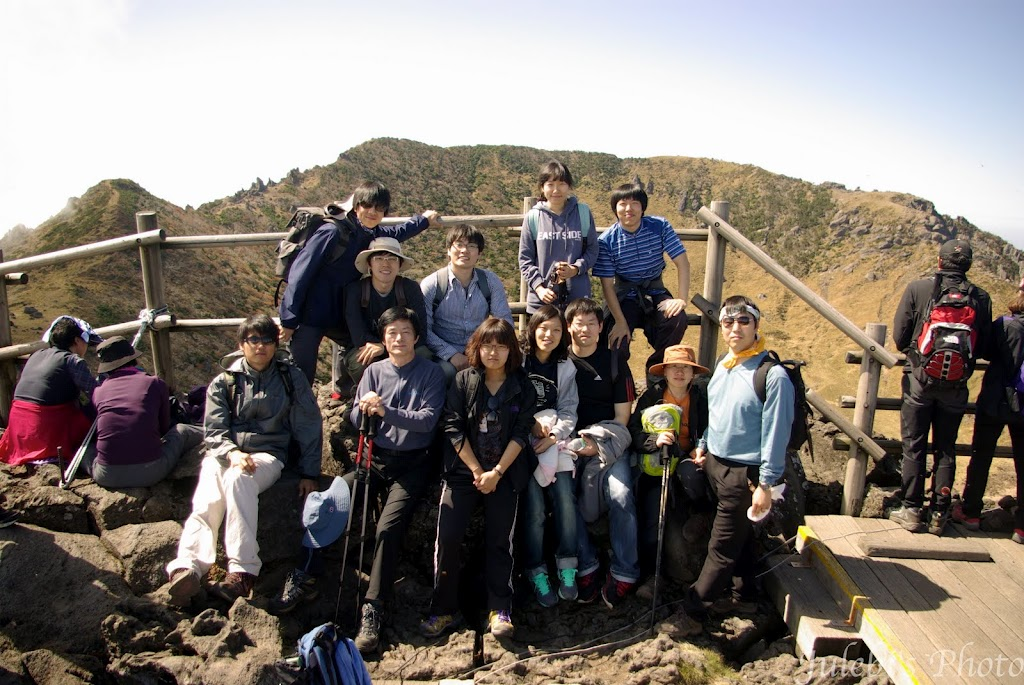
\includegraphics[width=0.85\textwidth]{./Figures/team-lee.jpg}
\legend{{\textsf{이명균 교수님팀---2011년 가을 한라산 등반}}}
\end{center}
\end{figure}
이명균 교수님 팀은 관측 우주론 (Observational Cosmology) 팀으로 천문학과 대학원에서 가장 규모가 큰 팀 중 하나입니다. 인자한 미소와 따뜻한 마음을 보여주시는 이명균 선생님의 지도 아래 2014년 1월 현재,  6명의 박사 과정생, 2명의 통합 과정생이 마치 형제들(!, 유경아 미안…)처럼 똘똘 뭉쳐 연구하고 있습니다.

관측 우주론 팀의 연구 분야는 1) 가까운 우주의 은하들 안의 AGB 별 2) 우리 은하의 산개 성단 및 구상 성단 3) 외부 은하의 성단계, 4) 외부 은하의 HII region, 5) 막대 은하의 형성과 진화 6) 은하 진화와 은하 환경의 관계 7) 다양한 환경에서 활동성 은하핵 특성 등으로 관측 우주론을 광범위하게 아우르고 있습니다. 이러한 주제에 대하여 주로 다양한 파장에서 얻은 측광 자료 분석과 보조적으로 분광 자료 분석을 통해 연구를 수행하고 있습니다.

관측 우주론 팀은 천문학과 대학원에서 팀 활동이 가장 활발한 팀입니다. 일단 매주 4시간 (ㅎㄷㄷ)에 이르는 팀 미팅을 통해 서로의 연구에 대한 열정적인 토론이 이루어집니다. 교수님과 학생들은 수시로 면담을 통해 연구 진행 상황을 논의하고, 졸업한 선배들과도 skype 등을 이용해 지속적인 토의 시간을 같습니다. 또한 1년에 한 두 차례 팀 워크샵을 개최하여 열띤 토론과 함께 아름다운 강산 (ex. 지리산, 울릉도, 제주도) 곳곳을 누비며 호연지기를 기르기도 합니다. 특히 등산에 있어서는 교수님의 지도 아래 모두가 달인이 되어가고 있습니다. 전국 명산들의 최고봉을 오르며 심신을 다스리며 팀워크를 다지고, 연구 의욕을 불사릅니다. 또한 정기적인 회식으로 팀 구성원들 사이의 돈독한 정을 자랑하기도 합니다. 조금 더 자세한 정보는 관측 우주론 팀 홈페이지(\url{astro.snu.ac.kr/~obscos}), 이명균 교수님의 홈페이지(\url{astro.snu.ac.kr/~mglee})를 통해 확인할 수 있습니다.

\subsubsection{박용선 교수님 팀}
박용선 교수님 팀은 성간 분자선을 관측하고 수치계산을 해서 은하 내 천문현상을 연구하고 있습니다. 또한  230GHz 전파망원경 (SRAO)을 운영하고 있으며, 천문기기개발을 하고 있습니다. 현 구성원은 교수님과 5명의 박사과정 학생, 2명의 석사과정 학생입니다.

우리 팀은 CO, CS를 비롯한 여러 분자선들을 SRAO, KVN등의 전파망원경을 이용하여 관측하여 분자운의 특성, 메이져선 관측을 통한 만기형 별의 특성, 복사 전달 방정식을 이용한 광 해리지역의 시뮬레이션을 주제로 연구하고 있으며, 미세전자기계거울(MEMS)을 이용한 적응 제어 광학계(Adaptive Optics)개발, 여러 배열 안테나의 빔을 적절하게 형성하여 태양풍을 측정하는 시스템 개발을 수행하고 있습니다. 우리 팀의 연구원들은 대부분 48-1동 전파천문대에서 생활하고 있고, 한 달에 한 차례 전파천문대에서 팀 미팅을 갖습니다.

\subsubsection{채종철 교수님 팀}
% \begin{figure}
% \centering
% \hspace*{\fill}
% \includegraphics[width=0.48\textwidth]{./Figures/2.jpg} \hfill \includegraphics[width=0.48\textwidth]{./Figures/3.jpg}
% \hspace*{\fill}
% \legend{(왼쪽) {\textsf{교수님 생신날 졸업한 선배들과}} (오른쪽) {\textsf{2012년 겨울}} } \label{fig:mult1}
% \end{figure}
\begin{figure}
\centering
\begin{minipage}{0.50\textwidth}
  \centering
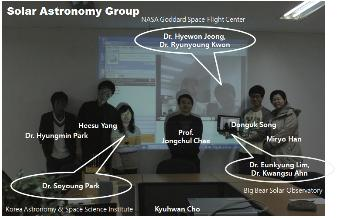
\includegraphics[width=\textwidth]{./Figures/team-chae-1.jpg}
\legend{{\textsf{채종철 교수님 생신 선배들과 함께}}} \label{fig:mult2}
\end{minipage}
\hfill
\begin{minipage}{0.48\textwidth}
  \centering
 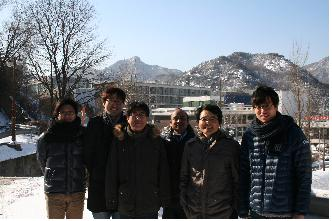
\includegraphics[width=\textwidth]{./Figures/team-chae-2.jpg}
\legend{{\textsf{채종철 교수님 팀---2012년 겨울}}} \label{fig:mult3}
\end{minipage}
\end{figure}

채종철 교수님 팀은 천문학과에서 유일하게 낮에만 관측을 할 수 있는 태양천문학 그룹(SNU Solar Astronomy Group)으로 현재 미국 빅베어 태양천문대 및 한국 천문연구원과 함께 태양의 광구, 채층, 그리고 코로나에서 일어나는 다양한 현상들을 분석 연구하고 있습니다. 현재 우리 팀의 구성원은 지도 교수님이신 채종철 교수님과 박사 후 연구원 2명을 비롯하여 박사과정 1명, 석·박 통합과정 2명과 석사과정 1명이 소속되어 있습니다.

또한 우리 팀은 태양의 관측 연구 이외에도 천문학 연구에 있어 매우 중요한 관측 기기에 대해서도 관심을 가지고 직접 개발하고 있으며, 2010년에는 고속 이미지 태양 분광기(FISS: Fast Imaging Solar Spectrograph)를 우리 팀에서 자체 개발하여 미국 빅베어 태양천문대(1.6m 태양망원경)에 설치를 하였습니다. 2010년 이후, 매년 6, 7, 8, 9월 약 4달 동안 우리 팀원들이 직접 가서 FISS를 사용한 관측이 이루어지고 있으며, 이 자료들을 사용하여 현재 좋은 결과를 얻고 있습니다. 

우리 팀은 매주 한 번의 팀 미팅을 통해서 서로의 연구 결과에 대한 다양한 토론을 하고 있으며, 매주 한번 있는 논문 쓰기 연습 시간을 통해서 논문 작성법에 대한 공부를 하고 있습니다. 또한 2주에 한번 있는 한국 천문연구원과의 미팅을 통해서 서로의 연구 활동을 공유하며, 미국 빅베어 태양천문대 및 한국 천문연구원과의 워크샵을 통해서 연구 활동 및 결과 그리고 관측 기기 개선을 위한 정보를 공유합니다.

채종철 교수님 연구실은 19동 310호에 위치하고 있으며, 연구 분야에 대한 자세한 정보는 다음을 참고해 주세요. 교수님 홈페이지 : \url{http://astro.snu.ac.kr/~chae} , FISS 홈페이지 : \url{http://fiss.snu.ac.kr}

\subsubsection{임명신 교수님 팀}
\begin{figure}
\begin{center}
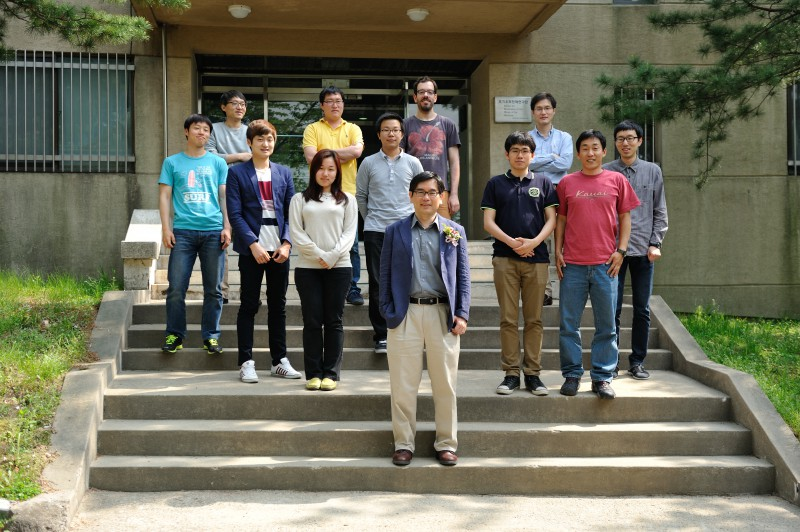
\includegraphics[width=0.85\textwidth]{./Figures/team-im-2014-1.jpg}
\legend{{\textsf{임명신 교수님 팀---2013년 스승의 날}}}
\end{center}
\end{figure}
임명신 교수님은 초기 우주 천체 연구단(Center for the Exploration of the Origin of the Universe, CEOU)의 단장님 입니다. 초기 우주 천체 연구단은 서울대의 김웅태 교수님, 경희대의 박수종 교수님 연구팀과 함께, 초기 우주에 존재하였던 (빅뱅 이후 ~1Gyr 지났을 때) 천체들을 발견하고 그것들의 성질을 연구하는 Infrared Medium-deep Survey (IMS)를 진행하고 있습니다. 
우리 팀에는 현재 교수님 이외에 박사후연구원 3분을 비롯하여 대학원생 8명, 행정간사 1명이 소속되어 있습니다.

우리 팀의 연구 대상은 가까운 우주에서부터 멀리 있는 우주, 즉 초기 우주에 존재하는 보통 은하, 활동성 은하, 초거대질량 블랙홀, 감마선 폭발 천체 등입니다.
\begin{packed_enum}
\item 보통 은하(Normal Galaxies): 무거운 타원은하(Elliptical Galaxies)의 색구배(Color Gradient)와 질량 대 광도 관계(Fundamental Plane), 매우 붉은 은하(Extremely Red Objects)의 군집. 초기 은하단의 발견(Overdensities of Proto-Clusters), 초은하단(Super Cluster)의 성질 연구. 초기 우주 별생성은하(Star-forming Galaxies)의 별 탄생률(Star Formation Rate) 연구, 표면밝기가 어두운 은하(Low Surface Brightness Galaxy) 연구.
\item 활동성 은하(Active Galaxies) 및 초거대질량블랙홀(Super Massive Black Holes): 초기 우주의 퀘이사(Quasars) 발견, 초거대블랙홀의 질량 진화, 초기 우주의 은하간 물질(Intergalactic Medium) 이온화 연구. 적외선 방출선을 이용한 블랙홀 질량 측정법, 붉은 활동성 은하핵(Red AGN) 발견 및 연구, 전파 활동성 은하핵 연구(Radio AGN Properties). 활동성 은하의 별 생성률 지표(Star Formation Rate Indicator). 은하 합병이 블랙홀 질량에 미치는 영향 연구.
\item 감마선 폭발 천체(Gamma Ray Bursts): 감마선 폭발 천체의 가시광 및 적외선 후속 관측(Follow-up). 블랙홀 활동 모니터링(Long Term Monitoring of BH Ignition). 감마선 폭발 천체가 속해있는 은하의 먼지의 기원(Dust property of GRB Host Galaxy).
\item 외부 은하에서 발견되는 초신성: 초신성 후속 광도 변화 관측(SN Follow-up Observation). M101은하에서 터진 초신성 모니터링(M101SN Observations).
\end{packed_enum}
이러한 천체들을 지상의 다양한 망원경(주로 UKIRT, McDonald 2.1m, Maidanak 1.5m, LOAO 1.0m 등) 혹은 우주 망원경(AKARI 등)을 이용하여 관측을 합니다. 우리의 연구에 필요한 기기를 직접 개발하기도 하는데, 예를 들어, 우리가 만든 SNUCAM이 Maidanak 1.5m 망원경에, CQUEAN이 McDonald 2.1m 망원경에 부착이 되어 있습니다. 또한 우리 팀은 매일 아침 arXiv 에 올라오는 논문들을 리뷰합니다. 흥미로운 논문들을 같이 읽고 내용에 대해 의논 합니다.

우리 팀의 연구실은 다른 팀들과는 다르게 19동이 아닌 45동에 위치하고 있습니다. 연구 분야에 대한 자세한 정보는 다음을 참고해 주세요. (팀 홈페이지: \url{http://astro.snu.ac.kr/~exact} , CEOU 홈페이지: \url{http://bigbang.snu.ac.kr} , 교수님 홈페이지: \url{http://astro.snu.ac.kr/~mim})

\subsubsection{김웅태 교수님 팀}
김웅태 교수님 팀은 천문학과에서 좀처럼 찾기 힘들다는(?) 이론, 수치계산 그룹(CNTAG: Computational aNd Theoretical Astrophysics Group)으로 초기우주천체연구단(CEOU)에 속해 있습니다. 현 구성원은 교수님과 3명의 박사과정 학생, 1명의 석사과정 학생입니다.
  김웅태 교수님을 비롯한 그룹원들은 이론과 수치계산의 방법을 이용해 천문학의 다양한 문제를 연구합니다. 최근의 연구 주제는 막대 은하, 막대-나선 은하에서의 기체역학과 별 형성, 기체 원반의 중력 불안정, 우리 은하의 나선팔 구조 등이며, 특히 은하 기체 역학, 별 형성의 연구는 미국 프린스턴대학 대학의 이론, 수치계산 그룹들과 공동연구를 진행하고 있습니다. 그 밖에도 나선팔에서의 거대분자구름 형성, 동역학적 마찰, 격변 변광성에서의 질량 교환, 은하단 기체역학 등의 여러 문제에 관심을 갖고 있습니다.
  그룹원들은 한 달에 한 번씩 갖는 팀미팅을 통해 서로의 연구 활동과 관심사를 공유하며, 매년 하반기에는 KNAG(Korean Numerical Astrophysics Group) 정기 미팅에 참가하기도 합니다.

더 자세한 정보는 교수님 홈페이지 (\url{http://astro.snu.ac.kr/~wkim}), CNTAG 홈페이지 (\url{http://astro.snu.ac.kr/cntag})에서 찾아볼 수 있습니다.

\subsubsection{이정훈 교수님 팀}
 이정훈 교수님 팀은 한국의 여러 대학의 천문학과에서 찾아보기 힘들다는 이론 우주론 팀입니다. 현재는 교수님과 1명의 석박사 통합과정 학생으로 구성되어 있습니다. 이론 우주론 팀에서는 주로 우주의 거대구조의 특성과 진화를 이론적으로 연구하여 우주표준모형($\mathrm{\Lambda CDM}$: Lambda-Cold Dark Matter Model)의 유효성을 검증하는  연구를 합니다. 은하나 은하보다 더 큰 거대구조 (은하단, 필라멘트, 보이드)의 질량함수 및 분포의 이론적 모델을 세우고 관측적, 수치적 자료를 함께 이용하여 암흑물질과 암흑 에너지, 우주 초기 밀도장의 성질을 규명합니다. 
 또한 우주 표준모형으로 설명되지 않는 여러 관측적인/ 수치적 현상을 설명하기 위해 기존의 모형의 보완 및 새로운 모형의 제안과 검증 과정이 이론 우주론 팀의 주요 연구 주제 중 하나입니다. 미국, 독일, 캐나다 등지의 저명한 우주론 학자들과 활발한 공동 연구를 펼치고 있습니다. 학생들의 연구는 주로 교수님과의 개별 면담을 통해 진행되고 한 학기에 한두번 정도의 비정기적인 팀 미팅을 갖습니다. 필요에 따라 우주론 팀의 학생들끼리 모임을 갖기도 하였는데, 이 또한 비정기적인 모임으로 자세한 정보는 이론 우주론 팀에 소속된 학생에게 문의해주시기 바랍니다.

\subsubsection{우종학 교수님 팀}
우종학 교수님 팀은 우주에서 가장 강력한 에너지원인 거대질량블랙홀들과 은하의 형성 및 진화에 대해 연구하는 거대블랙홀 연구실(AGN Research Group) 입니다. 현 구성원은  우종학 교수님과 박사 후 연구원 한 분과 박사과정 2명, 석사과정 1명입니다.

거대질량블랙홀은 은하 중심에 위치하는 것으로 알려진 질량이 태양질량의 백만배 가량을 넘어가는 천체입니다. 이러한 블랙홀로 가스가 유입될 때 일어나는 현상인 활동성은하핵(AGN:Active Galactic Nucleus)은 수천억 개의 별들로 이루어진 은하 전체의 밝기보다 열배에서 백배 가량 더 많은 에너지를 방출합니다. 거대블랙홀 연구실에서는 블랙홀과 AGN, 그리고 은하의 진화과정을 밝히기 위해 허블우주 망원경, Keck 망원경, Palomar 망원경, Lick 망원경, Subaru 망원경, SALT 망원경 (The Southern African Large Telescope) 등을 비롯한 다양한 관측기기를 이용하여 퀘이사, 세이퍼트(Seyfert) 은하, 전파 은하 등을 연구하고 있습니다.

저희 팀은 보통 매주 팀미팅을 가지고 있습니다. 팀미팅 시간은 주로 한 사람이 연구와 관련된 논문을 리뷰하고 이에 대해 각 팀원들과 교수님이 토의하는 방식으로 이루어집니다. 또한 간단히 연구결과를 이야기하는 시간도 있어 서로의 연구가 어떻게 진행되어가고 있는지를 알 수 있습니다. 
(우종학 교수님 홈페이지 : \url{http://astro.snu.ac.kr/~woo})

\subsubsection{이시구로 마사테루 (Ishiguro Masateru) 교수님 팀}
이시구로 선생님 팀은 태양계 천문학을 연구하는 팀입니다. 저희 팀은 한국에서 태양계를 공부하고 싶으신 학생들의 몇 없는 선택지 중 하나이고, 행성과 달을 제외한 태양계 천체를 공부하고 싶으신 분들께는 슬프게도(?) 유일한 선택지입니다. 2014년 봄학기에는 선생님 외에 기존의 학생 중 1명의 박사과정 학생과 1명의 석사과정 학생, 1명의 통합과정 학생이 남아있을 것입니다.

태양계 천문학 연구에서는 여타의 천문학 분야보다 훨씬 자세한 관측 자료를 얻을 수 있으며, 제한되나마 실제 샘플도 획득할 수 있습니다. 그 결과, 여타의 분야보다 상대적으로 복잡하고 구체적인 모형이 제시, 검증되고 있습니다. 저희 팀에서는 이러한 상황에 대응하기 위하여 다양한 연구 방법을 이용하고 있습니다. 관측, 수치 실험, 기기 제작 등의 연구 방법을 종합적으로 동원하여, 넓은 안목에서 태양계의 구체적 존재 양태를 추적하고 있습니다. 실제로 8m 급 대형망원경, 다양한 2m 급 중형 망원경, 저희 팀에서 직접 제작 중인 소형 광학기기를 이용하여 딥필드에서 전천까지, 자외선에서 적외선까지, 측광, 분광, 편광 관측을 수행하고 있으며, 이와 병행하여 수치 실험도 동시에 진행되고 있습니다. 지금 입학하시는 분이 박사학위를 준비하시게 될 수년 후에는 선생님이 개발에 깊이 참여하고 있는 소행성 탐사선 Hayabusa II가 획득한 자료도 우선적으로 이용할 수 있을 것입니다.

현재 저희 팀에서 수행하고 있는 구체적 연구 주제를 예로 들면 다음과 같습니다.
\begin{enumerate}
\item 지구 근처에 존재하는 천체들의 기원과 특징은 무엇인가?
\item 혜성과 소행성이 충돌을 겪으면 어떠한 일이 발생하는가?
\item 태양계에 존재하는 티끌의 구체적 기원은 무엇인가?
\item 혜성과 소행성에서 발생한 티끌들이 그 후 어떻게 진화하는가?
\end{enumerate}
위와 같은 연구를 종합하여 태양계의 기원과 진화를 종합적으로 이해하는 것이 저희 팀의 목적입니다. 물론 구체적인 세부 주제는 계속하여 추가, 변경되고 있습니다.

저희는 보통 한 주에 한 번씩 3$\sim$4시간의 팀 미팅을 갖고 있으나, 얼마든지 변경의 여지가 있습니다.

\subsubsection{사샤 트리페 (Sasha Trippe) 교수님 팀}
사샤 트리페 교수님은 우리 과 외국인 교수님 투 톱 중 한 분으로 독일에서 박사학위를
받으신 후, 프랑스 IRAM에서 박사후과정을 거쳐 2011년에 서울대에
부임하셨습니다. 현재 네 명의 석박통합과정생을 두고 계시고, 연구는 주로 활동성
은하핵(AGN)을 전파영역으로 분석하여 수행하고 있습니다. 연구수행에는 주로 21m
망원경 세 개로이루어진 한국 VLBI망(KVN)과, 한국(KVN)-일본(VERA: 20m 망원경 7개)
연합 VLBI망(KaVA)을 이용하고 있습니다. 또한 교수님은 Modified Newtonian
Dynamics에도 관심이 있으시고, 기기 개발 방면에도 흥미를 갖고 계십니다. 교수님
홈페이지를(\url{astro.snu.ac.kr/~trippe}) 방문하시면 찾아보시면 재미있는 내용들을
찾아보실 수 있습니다.


\subsubsection{윤성철 교수님 팀}
윤성철 교수님 팀은 국내에 몇 없는 Stellar Astrophysics, 즉 항성의 내부 구조 및 진화, 탄생과 죽음을 연구하는 팀입니다. 윤성철 교수님은 2013년에 부임하셨고, 2014년 초 현재 석박통합과정생 두 명이 소속되어 있습니다. 교수님이 매우 젊으시고 부임 초기이시기 때문에 굉장히 열려있으시고 열정적이시며, 항성진화 뿐만 아니라 다양한, 말그대로 `다양한’ 분야에 폭넓은 관심을 갖고 계십니다.

현재는 우주 초기의 별(Pop III)의 탄생이나 He별의 진화와 같은 다양한 항성들의 진화뿐만 아니라, Type Ib/ Ic 초신성 폭발이 발생할 수 있는 조건과 같은 항성 전반과 관련된 총체적 특성들을 항성진화 모델통해 컴퓨터 계산으로 연구하고 있습니다. 

저희는 보통 매주 금요일에 팀미팅을 갖고 있으며, 이 외의 정보에 대해서는 교수님 홈페이지(\url{http://astro.snu.ac.kr/~yoon/home/})에서 찾아보실 수 있습니다.

\vspace{0.05\textheight}

\section{강의 소개 및 수업 관리}
대학원 합격의 기쁨을 누리기도 잠시, 신입생 여러분에게는 정식으로 입학하기 전에 미리 결정하고 해야 할 일들이 기다리고 있다. 그 중 빠뜨릴 수 없는 것은 바로 학기가 시작되면 어떤 수업을 들어야 하는지 알아보는 것이다. 새롭게 시작되는 대학원 생활을 앞두고 의욕에 가득 차 있을 당신! 하지만 첫 학기부터 단추를 잘 못 꿰게 된다면 억울한 일이 아닐 수 없다. 강의 정보 확인은 서울대학교 정보 광장 (\url{http://my.snu.ac.kr})에서 수강 편람에 들어가 강의 계획서를 열람하는 것이 가장 확실한 방법이지만, 한 학기에 개설되는 수업의 종류가 다양하기 때문에 사전 정보가 없이 선택하기란 쉬운 일은 아니다. 따라서 이 챕터에서는 신입생의 수업 선택에 도움을 주고자 간단한 강의 소개와 이수 규정에 대해 설명하도록 한다.

석박통합 과정의 졸업 이수 기준 학점은 총 60학점이다. 대학원에서는 수업과 더불어 연구도 진행해야 하기 때문에 통합과정의 수료를 6학기로 보고 있다면 한 학기에 10학점을 들어야 하기 때문에 빠듯할 수 있다. 이를 돕기 위해 18학점의 논문연구교과목과 6학점의 콜로퀴움 수업을 두어 24학점의 부담을 덜어주고 있으니 이를 참고하여 글을 읽자.

적합한 선택을 하기 위해서 가장 먼저 수업 종류에 대해 알아보자. 천문학과의 수업은 크게 일반 교과 수업과 세미나 수업으로 나누어 볼 수 있다.
\begin{packed_item}
\item 교과 수업은 학부 과정에서 수강했던 수업과 크게 다르지 않고 천문학 연구를 위한 배경지식을 습득하는 데에 주력하게 되며, 일반적으로 선생님의 강의로 수업이 구성된다. 수업 평가는 주로 시험을 통해 이루어지며 부가적으로 과제와 수업 참여도를 반영하기도 한다.
\item 반면 세미나 수업은 강의보다는 학생들의 발표와 토론이 주가 되는 과목이다. 자신의 연구 주제를 가지고 수업이 진행되는 동안 스스로 연구를 진행해야 하기 때문에 시험에 대한 단기적인 스트레스는 없는 편이지만 지속적인 발표와 레포트로 연구 능력과 성실함을 요구한다.
\end{packed_item}
 따라서 정해진 규정은 없지만 일반적으로 1학년 때는 주로 교과 과목에 투자를 하고, 1년 정도 지난 후에 세미나 수업을 들을 것을 추천하고 있다. 특강 및 세미나 수업을 듣기 전에 관련 수업을 미리 들어두는 것이 좋다 (예: 천체분광학 및 실험 $\rightarrow$ 천체분광세미나 ). 단, 지도 교수님에 따라 세미나 수업을 권유하는 분도 계시기 때문에 수강 신청 전, 팀 선배에 조언을 구하는 것은 언제나 도움이 된다는 점을 잊지 말자.

이와는 별도로 천체물리세미나(콜로퀴움) 수업과 논문연구교과목이 있다. 천체물리세미나는 학기 중 매주 목요일과 추가로 있는 특별 콜로퀴움에 참석하는 것으로 수업을 대체하는데, 박사과정 중 2번 신청할 수 있으며 담당 선생님에 따라 레포트를 요구하기도 한다. 논문연구교과목은 총 18학점을 대체할 수 있는 수업으로 강의나 발표 없이 개인의 연구 역량을 증진시키고 연구 시간을 확보하는 데에 도움을 준다. 따라서 통합과정 중 교과 과목과 세미나 수업으로 이수해야 할 학점은 총 36학점으로 12과목이 되겠으며 이는 6학기 동안 매 학기 두 과목을 들어야 하는 수준이다.
교과 수업의 간략한 설명은 학과 홈페이지의 \href{http://astro1.snu.ac.kr/home/kor/info/subject_dahakwon.asp?globalmenu=3\&localmenu=5}{학사정보 탭}에 있으니 참조하자. 
이 중 첫 학기 추천 과목은 봄 입학 기준 천문관측법과 천체물리학, 가을 입학 기준 외부은하와 우주론, 성간 물질과 항성역학 및 중력이며, 위 수업들은 논문자격시험의 필수 과목이기도 하다. 
이 밖에도 연구팀을 소개하는 신입생 대상 수업 ‘현대 천문학 특강’ 이 있으며, 배경 지식이 부족하다고 생각될 경우 학부 수업이나 타과 수업을 수강할 수도 있다.

\section{컴퓨터 세팅, 계정 만들기}
\subsection{하드웨어 마련하기}
책상 위에 펜과 종이, 커피 한 잔만 있으면 논문이 써지는 순수 이론가가 아니라면, 대부분의 연구 활동은 컴퓨터에서 이루어진다. 그러니 무엇보다 개인컴퓨터를 마련하는 것이 우선이다. 개인컴퓨터는 팀에서 지원해주기도 하니 반드시 미리 선배들을 통해 알아보자!

연구용으로 컴퓨터를 장만할 때 고려해야 할 사항이 있다. 시뮬레이션을 돌리거나 하는 많은 연산이 필요한 작업이 예상된다면 CPU 성능과 RAM 용량이 중요할 것이다. 만약 많은 양의 데이터를 처리해야 한다면 하드의 용량이 중요할 것이고, 이미지를 주로 봐야 한다면 큰 모니터 혹은 듀얼 모니터가 있으면 좋을 것이다. 하지만 만약 팀이 소유하거나, 외부 기관이 소유한 서버에서 작업을 주로 하게 된다면 CPU의 성능이나 하드의 용량은 그다지 중요하지 않을 수도 있다. 이와 같은 사항은 같은 팀의 선배나 지도교수님과 상의해보는 것이 가장 좋을 것이다.

\subsubsection{IP 신청}
학교 어디에서든 무선인터넷은 콸콸콸 터지고 19동에서도 astro 무선인터넷을 사용할 수 있다 (비밀번호는 선배에게 물어보라). 그러나 데스크톱의 네트워크 연결을 위해 IP는 반드시 필요하다. 개인 IP는 정보 광장에 접속해 신청할 수 있다. 그리고 IP신청을 하면 지도교수님에게 메일을 보내어 담당학생이 맞는지 확인을 한 후 IP를 발급해준다. 그러니 지도교수님에게 미리 말씀을 드리는 것도 잊지 말자. (서울대학교 포털 (\url{http://my.snu.ac.kr}) 로그인 --- 스누인지원 --- IT 서비스 --- IP/Domain 신청/반납)

\subsubsection{포트 신청}
집에서도 연구하는 성실한 학생임을 지도 교수님께 어필할 기회가 있다. 
바로 자신의 데스크탑의 포트를 여는 것이다. IP 신청과 마찬가지로 포트 신청을 하면 지도 교수님의 확인 후에 포트를 열어준다.
이 경우 지도 교수님께서, 아 이 학생은 집에서도 연구하는 성실한 학생이구나 하며 흐뭇한 미소를 지으실지도 모른다.
일단 IP 신청을 마치고 받은 후에 IP와 비슷한 경로를 통해 들어가 자신의 IP에 원하는 포트를 열어달라고 요청하자. 
(\url{http://my.snu.ac.kr}) 로그인 --- 스누인지원 --- IT 서비스 --- IP/Domain 신청/반납)
보통 많이 사용하는 포트는 21번 (FTP), 22번 (SSH), 5900 (VNC) 정도이다. 이 정도 포트를 열어두면 집에 있는 컴퓨터로 학교 데스크탑에 원격 접속하여 신나는 연구 생활을 즐길 수 있다!!! 

\subsubsection{공용 네트워크 프린터 설정}
학과에서 공용으로 사용하는 프린터는 3층 행정실 옆에 위치하고 있다. 연결 방법은 운영체제마다 조금씩 차이가 있다. 잘 모르겠으면 인터넷을 찾아보거나, 행정실 조교님 혹은 주변 선배에게 물어보면 친절히 잘 알려줄 것이다. 아! 왠만하면 잊지 말고 양면 인쇄 설정엔 체크하여 자원을 아끼자. 
\begin{packed_item}
\item 흑백프린터 - HP LaserJet 4515x (IP: 147.46.20.148)
\item 컬러프린터 - HP Color LaserJet 4700 (IP: 147.46.135.143)
\end{packed_item}

\subsection{소프트웨어 마련하기}
하드웨어를 마련했다면 이제 소프트웨어를 설치해보자. 천문학과에서 기본적으로 사용하는 프로그램은 다음과 같다.
\begin{packed_item}
\item IDL : 파일 입출력, 데이터 분석을 위한 프로그래밍 언어로 가장 널리 쓰인다.
\item IRAF : 리눅스에서 천문학 관련 작업(Task)들을 쉽게 처리 할 수 있도록 Package화 해놓은 Tool
\item PYTHON : 천문학계에서 IDL과 쌍벽을 이루는 고급 프로그래밍 언어, PYTHON으로 IRAF Task 들을 구현해 놓은 PYRAF라는 것도 있다.
\item LaTeX : 주로 논문을 작성하게 될 때 쓰게 되는 문서 작성 도구
\end{packed_item}
각 팀별로 사용하는 프로그램들이 다르고, 개인의 취향이 있으니 미리 알아보고 준비하도록 하자. 프로그램에 대한 자세한 내용은 3장에서 다루고 있으니 3장을 자세히 살펴보도록 하자.

팀 내 서버에서 주로 작업을 하게 된다면 원격 접속 프로그램이 필요하다.
\begin{packed_item}
\item Xmanager : 아래에서 설명하고 있는 캠퍼스 라이센스 S/W 중 하나로서 SSH protocol로 서버에 접속할 수 있는 환경을 제공해준다. (Xftp, Xstart 등)
\item VNC :  Remote Terminal (주로 자신의 Desktop) 에서 서버의 자신의 작업 공간 (주로 서버의 자신 계정의 홈페이지) 으로 접속하여 작업할 수 있게 해주는 프로그램이다.  VNC의 강력한 점은 Terminal로 접속하는 방식과 달리 자신이 했던 작업을 그대로 다음번 접속 때 이어서 할 수 있다는 점이다. (\url{http://www.realvnc.com})
\end{packed_item}

\subsubsection{캠퍼스 라이센스 S/W 배포 시스템}
교내 IP로 접속한 경우 학교에서 지원하는 각종 소프트웨어를 다운받을 수 있다. 학교 사이트에 접속하면 더욱 쉽고 편리하게 다양한 소프트웨어(Window, MS Office, Adobe 프로그램들, 보안프로그램 etc)를 다운받을 수 있다. (서울대학교 포털 로그인(\url{http://my.snu.ac.kr}) --- QUICK MENU --- SW 다운로드)

\subsection[E-mail 계정 만들기]{E-mail 계정 만들기\footnote{이준협 선배님의 매뉴얼로부터 \cite{manual_ljh}}}
천문학과에 입학하여 가장 먼저 필요한 것 중 하나는 학과서버에 자신의 계정을 만드는 것이다. 학과 사무실에 자기 계정으로 쓸 아이디를 적어내면 그 아이디로 계정을 만들어준다. 그런데 자기 이름의 이니셜을 이용해서 만들라는 권장사항을 무시하고 원래 인터넷에서 즐겨 쓰던 아이디를 고집하는 사람이 꼭 매년 한두명씩 나온다. 천문학을 중간에 그만둘 계획을 가지고 있지 않다면 절대 그러지 말기 바란다. 여기에 만드는 계정은 그대로 자신의 공식적인 메일주소가 되며 논문을 쓰면 논문에 그 메일주소를 실어야 된다. 그리고 어떤 천문학자도 자신의 이름과 무관한 이상한 아이디로 공식메일을 사용하지는 않는다. 가령 자신이 인터넷상에서 \texttt{sexyking}라는 아이디를 사용하고 있었다고 해서 그대로 학과계정을 만들면 논문저자 이름 밑에다가 \texttt{sexyking@astro.snu.ac.kr} 이라고 써야 하는데, 그걸 읽는 사람들이 어떻게 생각할지 상상해 보라. 공식 계정답게 무난하고 품위 있는 아이디를 만들기 바란다. 예를 들어 이름이 홍길동이라면 \texttt{gdhong} 으로 하는 것이 가장 일반적이며, \texttt{ghong, gildong, honggd, hgd} 등등까지는 대체로 무난하다고 하겠다.

\section{학자금 마련하기}
\begin{itemize}
\item \textbf{장학금 신청 시기}: 매년 마다 조금씩 틀리지만 일반적으로 2학기는 5월 첫째 주, 다음 해 1학기는 11월 첫째 주에 장학금 신청 카드를 제출해야 한다. 신청하지 않으면 장학금을 받을 수 없다!
\item \textbf{장학금 종류}: 강의$\cdot$연구 장학금 (GSI), 수업료 및 입학료 면제 장학금, 근로 장학금, BK 장학금, 유학생 장학금, 대출학자금이자지원 장학금, 서울대학교 발전기금 장학금, 이공계 국가장학금, 글로벌 박사 펠로우쉽, 미래 기초과학 핵심리더 양성사업, 교외 장학금 (롯데, STX, KT\&G 등) 등 여러 가지 종류의 장학금이 있다. 장학금, 학자금 대출과 관련한 자세한 사항은 다음의 사이트들을 참고하자 (\url{http://scholarship.snu.ac.kr/}, \url{http://www.nrf.re.kr}).
\item 행정실 조교님께서 학생들이 받을 수 있는 학내, 외부 장학금과 관련한 메일을 항상 보내주시니 \textbf{\emph{메일함을 수시로 체크하자!}}
\end{itemize}

\subsubsection{올림피아드 조교}
학과 건물 내에 올림피아드 사무실이 위치하고 있기 때문에 종종 시험감독, 채점 조교를 모집할 때가 있다. 짧은 시간을 일하고도 짭짤한 수입을 얻을 수 있기 때문에 용돈 벌이에 좋을 것이다.


\section{주거 관련 정보}
\begin{packed_item}
\item 현재 대학원생들은 기숙사/서울대 입구/녹두/낙성대에 거취함. (물론 집이 가까운 사람은 집에 거주한다!)
\item 기숙사에 대한 자세한 정보는 사이트를 참고하자!! (\url{http://dorm.snu.ac.kr})
\item 기숙사 신청 기간을 놓치면 입사할 수 없으니  사이트를 수시로 체크하자!! 대부분 방학 전에 신청하므로 잊지말자!!
\item 천문학과 홈페이지에도 공고한다. 하지만 혹시 모르니 항상 사이트를 체크하자!!
\item 참고로 까다롭지 않지만 기숙사 입사조건이 있다. (성적, 건강검진, 보호자 거주지 등)
\item 아래의 그림은 기숙사 신청시 홈페이지이다. 아래의 그림에서 붉은색 BOX 안에 있는 내용을 체크하지 말자!! 대학원 신입생은 붉은색 BOX 안의 내용에 해당되지 않으므로 체크하면 기숙사 입사와 멀어진다. 경험자 있음..;;;
\item 기숙사에 떨어진 사람은 자취나 하숙을 하게 되는데 방 값은 일반적으로 서울대입구역=낙성대 $>$ 녹두(신림9동) 이다.
\item SNULIFE 사이트의 생활정보 카테고리에 스누복덕방에서 다양한 방을 알아 볼 수 있다. 링크: \url{http://www.snulife.com/housing}
\item 자취나 하숙보다는 기숙사를 추천하니 기숙사 입사를 위해 최선을 다하자!!
\item 더 자세한 정보는 서울대학교 생활 백서를 참고하자 (2009년 버전으로 현재와는 조금 다를 수 있다)!! 링크: \url{http://www.snuco.com/html/partner/partner_white_papaer.asp}
\end{packed_item}

\begin{figure}
\begin{center}
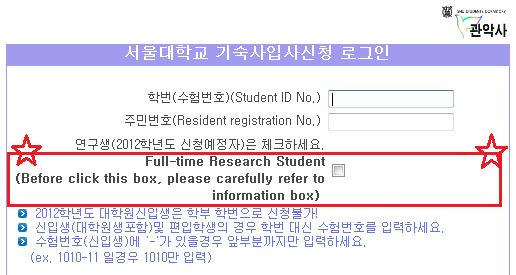
\includegraphics[width=0.85\textwidth]{./Figures/dorm.png}
\legend{{\textsf{붉은색 BOX 체크하지 말것!}}}
\end{center}
\end{figure}




\chapter{대학원에서 살아남기}
\epigraph{알아서 잘 ...}
{{\textsc{이명균 교수님}}}

\section{식당, 건물 및 캠퍼스 소개}
\begin{figure}
\begin{center}
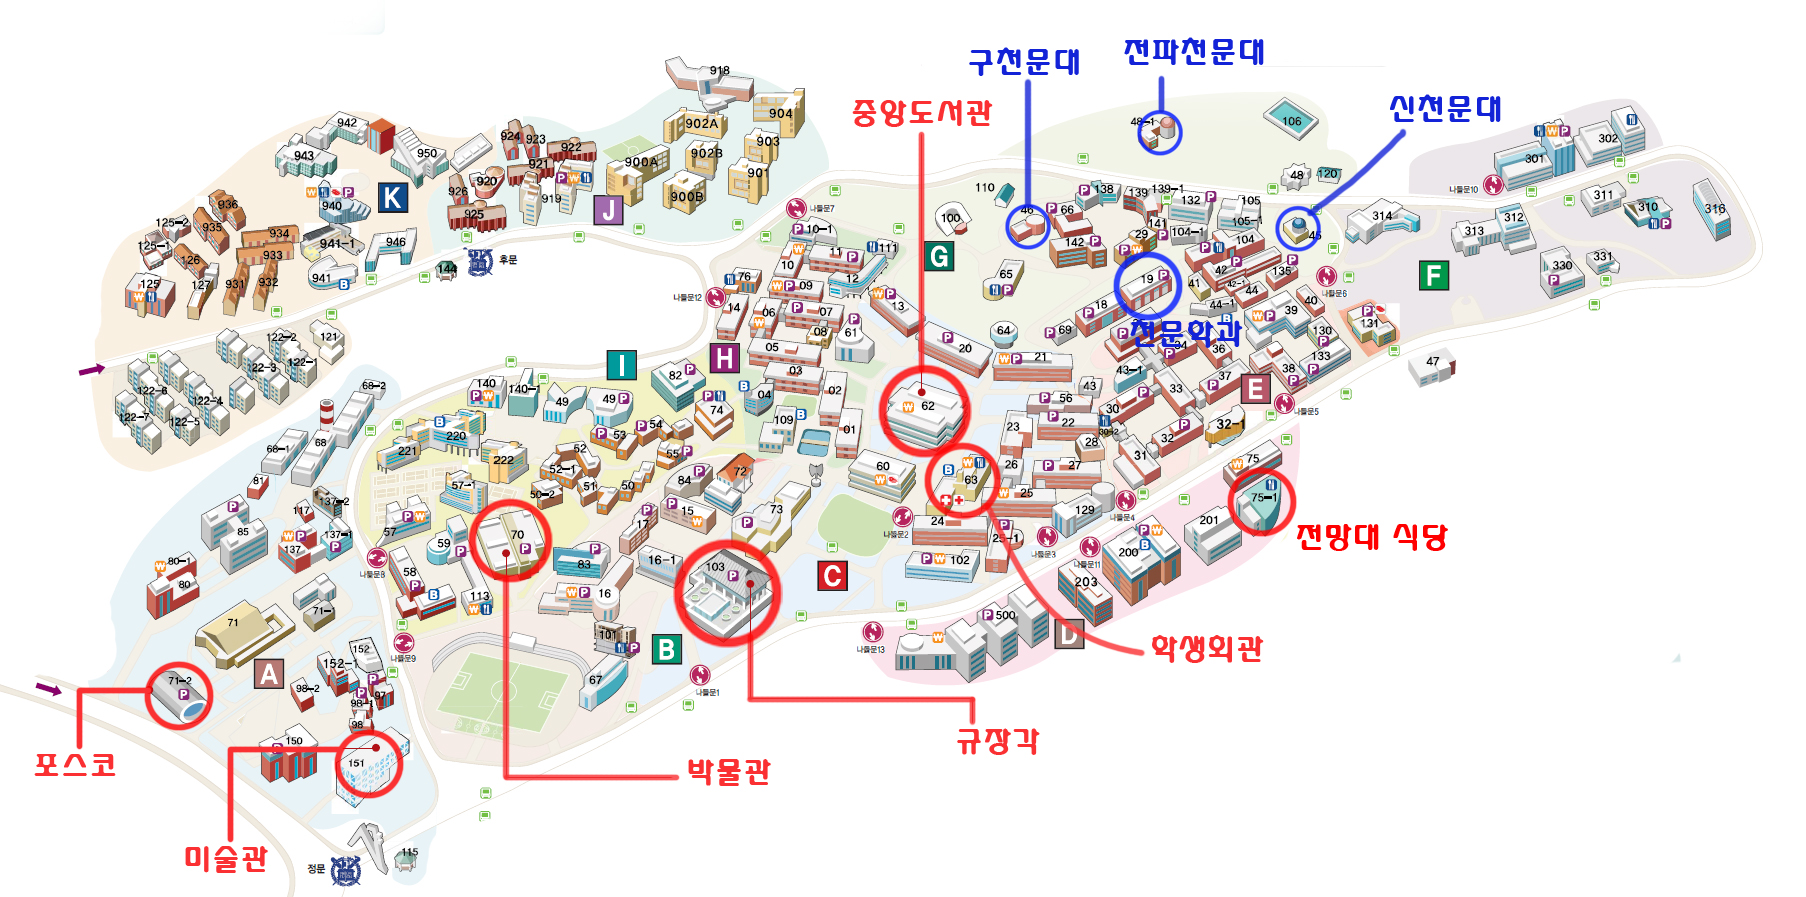
\includegraphics[width=0.95\textwidth]{./Figures/campus_map.jpg}
\legend{\textsf{캠퍼스 내 주요 건물}}
\end{center}
\end{figure}

\subsection{식당}
서울대학교는 신입생들이 (때로는 다닐 만큼 다닌 사람들도...) 가끔 길을 잃을 만큼
넓은 캠퍼스를 자랑한다.  그 넓이만큼 곳곳에 식당들도 많이 있다. 일단 다 먹고
살자고 하는 일이니 천문학과 대학원생들이 주로 이용하는, 혹은 이용가능한 식당에
대해 간단히 알아보자.\footnote{생활협동조합 직영 및 준직영 식당들의 메뉴 정보와
  운영시간 위치 등은 \url{http://www.snuco.com} 에서 자세히 확인할 수 있다.}
그외에 샤밥이라는 아이폰 어플과, inSNU라는 안드로이드 어플 등도 있으니
활용해보자.

\begin{description}
\item[\textsf{전망대(75-1동)}] \hfill \\
  천문학과 대학원생들의 주 이용 식당. 75-1동의 3, 4층에 위치하며 학생식당 중 19동에서 가장 가깝다. 보통 3층에 네 가지의 메뉴, 4층에 두세 가지의 메뉴가 제공된다.\\
  \hspace*{0.5cm}- 가격: 2500 / 3000 / 4000\\
  \hspace*{0.5cm}- 운영시간: 3층 - 11:00--14:00 / 4층 - 11:30--13:30, 17:00--19:00.\\
  \hspace*{0.5cm}- 주말은 토요일 점심만 4층이 운영되고 나머지는 휴관이다.\\

\item[\textsf{학생회관(63동)}] \hfill \\
  학생회관에 위치하는 식당으로 19동에서 갈 경우 식당으로 갈 때는 갈만하다는 생각이 들지만 올라올 때 많이 힘들다;; 학생회관인 만큼 주말까지 열려있으며 평일에는 저녁 9시까지 운영된다. 세 가지의 메뉴가 각각의 시간대별로 제공되며 지하에도 두 가지의 메뉴가 있다.\\
  \hspace*{0.5cm}- 가격 : 1700(B코너) / 2500 / 3000 \\
  \hspace*{0.5cm}- 운영시간 \hfill\\
  \hspace*{1cm} A코너 - 11:00--14:00, 16:30--18:30\\
  \hspace*{1cm} B코너 - 08:00--10:00, 11:00--14:00. 17:00--19:00\\
  \hspace*{1cm} C코너 - 10:00--16:30, 17:30--21:00\\
  \hspace*{1cm} 지하 - 11:00--13:00\\
  \hspace*{1cm} 주말 : 11:00--14:00, 17:00--19:00\\

\item[\textsf{공대간이식당(30-2동)}] \hfill \\
  전망대 만큼이나 가까이 위치한 식당이다. 짜장면, 짬뽕, 사천짜장이 고정 메뉴로 있으며 월~금 각각의 요일마다 정해진 덮밥 메뉴가 있다.\\
  \hspace*{0.5cm} - 가격 : 짜장면 2500원 / 짬뽕, 사천짜장, 덮밥류 3000원

\item[\textsf{솔밭식당(110동)}] \hfill \\
  거리상으로 상당히 가까우나 사실 잘 가게 되지는 않는 식당. 무려 학교보다도 더
  나이가 많은 식당이며 국수와 국밥류가 있다. 가끔 한 번씩 가기엔 나쁘지 않은
  식당.  2013년을 마지막으로 사라진다고 했는데... 아직은 열린 결말.

\item[\textsf{BBQ카페(32-1동 지하)}] \hfill \\
  치킨, 피자, 스파게티 등 여러 메뉴들이 있다. 학생식당들의 밥이 너무 먹기 싫은데
  밖에 나가기는 귀찮다거나 나갈 시간이 없을 때의 최선의 선택이다. 물론 치킨을
  좋아 할 경우에. 다른 외부업체들과 마찬가지로 학생할인이 된다.

\item[\textsf{반공연}] \hfill \\
  19동 뒷길로 올라가면 빠르게 갈 수 있는 식당으로 라면과 요일별로 정해진 밥이
  있다. 전망대 메뉴가 마음에 안들거나 라면이 급 땡길 때 가게 되는 식당이다.

\item[\textsf{기타}] \hfill \\
  이외에 서당골, 언덕방, 기숙사식당, 동원관식당 등의 학생식당이 있다. DOS TACOS,
  포베이, 비비고, 더키친, 파파이스 등의 외부업체들이 있다. 학교 탐방을 해 보고
  싶다거나, 다른 구역에 볼일이 있다거나 할 때 다른 식당들도 방문해보자.

\end{description}
\starbreak 밥만 먹고 살 수는 없다. 가끔 커피도 한 잔씩 마셔주고, 앉아서 이런 저런
이야기나 연구에 대한 토의도 할 수 있는 장소가 필요하다.
\begin{description}
\item[\textsf{The LAB(32-1동 1층)}] \hfill \\
  천문학과 대학원생들이 가장 많이 가는 곳이 아닐까 생각된다. 19동에서 전망대로
  가는 코스 중간에 위치하기 때문이다. 커피 등의 음료들과 간단한 간식거리들이
  있다.

\item[\textsf{Mug(공대신양)}] \hfill \\
  19동에서 아래로 내려가면 바로 만날 수 있는 공대신양에 위치한다. 연구에 지칠 때
  가끔 기분전환으로 갈 수 있는 곳이다. 손님(졸업한 선배 등)이 오면 자주 가는
  곳이기도 하다. 커피 등의 음료들과 샌드위치 등 간단한 음식들이 있다.

\item[\textsf{학생회관 스낵코너(63동)}] \hfill \\
  토스트 판매대, 토판이라고도 한다. 학생회관 1층 식당 옆에 위치하며 커피, 음료
  뿐만 아니라 샌드위치, 버거, 떡볶이와 순대까지 판매 한다. 위치가 위치이니 만큼
  항상 사람들로 붐빈다.

\item[\textsf{기타}] \hfill \\
  카페판코, 투썸플레이스, 파스쿠치 등의 카페들이 학교 곳곳에 위치한다.
\end{description}
\starbreak 간식거리를 살 수 있는 매점들 또한 곳곳에 위치하고 있다.
\begin{packed_item}
\item 일단 가장 접근성이 좋은 전망대 매점이 있다. 전망대 4층 입구쪽에 위치하고
  있으며 거리상으로 가장 가깝다기 보다는 보통 밥을 먹으러 가는 장소가 전망대이기
  때문에 가장 많이 이용되는 곳이다. 음료 및 과자 등 뿐만 아니라 간단한 문구류도
  구매할 수 있다.
\item 32-1동 지하(BBQ 옆)에 패밀리마트가 있다. 편의점이긴 한데 속지 말아야 할
  것은 11시가 되면 문을 닫는다.
\item 반공연 식당은 식당과 매점이 함께 운영되고 있다. 과자와 음료만 있다.
\item 중앙도서관 매점은 중앙도서관 터널, 뚜레쥬르와 같은 공간에 있으며 전망대
  매점과 마찬가지로 문구류 또한 구매할 수 있다. 편의점과 기숙사 매점을 제외하면
  학교내 매점 중 가장 오랜시간 열려있다. 밤 10시반까지 운영되며 시험기간엔
  연장운영이 된다.
\item 사회대 신양과 대학원 기숙사에는 각각 패밀리마트와 GS25가 있으며 이 두 곳은
  24시간 영업을 한다. 학부 기숙사(919동) 식당 옆의 매점은 새벽 두 시까지
  운영된다.
\end{packed_item}

\subsection{건물}
\begin{description}
\item[\textsf{학생회관(63동)}] \hfill \\
  학생들을 위한 시설들이 가장 많이 포함된 곳은 역시 학생회관이다. 매일 열려있는
  학생식당을 포함 보건소, 약국, 문구점, 서점, 은행 등 각종 시설들이
  있다. 천문학과 대학원생들은 학생회관을 갈 일이 실질적으로 별로 없긴 하지만
  학생회관에서 간단히 해결 할 수 있는 일들을 힘겹게 학교 밖으로 나가서 해결하는
  경우들이 간혹 있으니 학생회관에 어떤 것들이 있는지는 파악해 두는 것이 좋다.
\begin{packed_item}
\item 식당과 매점, 스낵코너
\item 보건소, 약국
\item 문구점, 서점
\item 농협, 신한은행
\item 복사/제본/인쇄
\end{packed_item}

\item[\textsf{중앙도서관}] \hfill
\begin{packed_item}
\item 중앙대출실은 도서관 4층에 위치하고있다(중앙도서관 터널은 3층!).
\item 평일 09:00$\sim$21:00 / 토요일 09:00$\sim$17:00 / 일요일 13:00$\sim$17:00
\item 대학원생의 경우 대출기간은 1개월이며 20권까지 대출이 가능하다.
\item 대출 연장은 2회까지 가능하다. 단, 주의할 점은 연장을 하면 한달이 추가가
  되는 것이 아니라 연장 순간부터 다시 한 달이 된다. 반납기한이 지나버리면 연장이
  불가능하며 다른 사람이 예약을 해 둔 경우에도 연장이 불가능하다.
\item 연체시 3일 이후부터 (이전 3일까지 소급하여) 1일/1권 당 100원의 연체료가
  발생한다. 연체료가 있을 경우 대여를 할 수 없으며, 연체료를 내지않으면 졸업도
  안시켜준다는 것 명심할 것.
\item 졸업시 유의할 점 : 졸업 시점에 대출 도서가 있으면 졸업 처리가 안된다. 잊지
  말자.
\item 간혹 빌린 책이 꼭 필요해서 반납 기한이 지난 것을 알면서도 '나중에 연체료
  내고 말지 뭐'라고 생각하고 반납을 안 하는 경우들이 있는데 이것은 양심을
  팔아먹는 일이다. 절대 해서는 안되는 행동이다.
\item 필요한 책이 있는데 비싸서 사기 힘들 경우 중앙 도서관에 구매 신청을
  하자. 연구팀에 따라서는 팀 예산으로 필요한 책을 자체 구매할 수 있기도 하다.
\item 영상자료실에서 영화를 볼 수 있는 시설도 있으며, 중앙대출실 로비에는 그 자리에서 읽을 수 있는 다양한 서적들과 심지어 만화책도 있다. (슬램덩크!)
\item 6개의 대형 열람실이 있다. 1$\sim$6층 중 4층을 제외한 각 층에 열람실이
  있으며 3층은 3A / 3B로 구분되어있다(입구는 동일).
\end{packed_item}
\starbreak 관악캠퍼스에는 중앙도서관 이외에
사회과학도서관/경영학도서관/국제학도서관/농학도서관/법학도서관이 있으며 찾는 서적
중 중앙도서관에 없는 책이 있는 경우도 있다(연구를 위해 찾는 책은 그런 경우가
없다고 봐도 무방하다;;;). 각 도서관의 대출 시간/방식에 맞춰 대출이 가능하다.

\item[\textsf{은행}] \hfill
  \begin{packed_item}
  \item 우체국 : 대학본부 측면
  \item 농협 : 39동/학생회관/자하연
  \item 신한은행 : 공대신양/학생회관
  \item 우리은행 : 500동/인문대신양
  \end{packed_item}
\item[\textsf{운동시설}] \hfill \\
  운동, 매우 중요하다. 중요성에 대한 설명은 더 하지 않겠다.
  \begin{packed_item}
  \item 공대 BK헬스장 : 19동에서 가장 가깝다. 비교적 작지만 거리에서 매우 큰
    이점이 있다.
  \item 포스코 : 헬스, 수영, 스쿼시 등을 할 수 있으며 정문 쪽에
    위치한다. 19동에서의 거리는 제법 멀지만 학교 오는 길에 운동을 하기엔 그리
    나쁘지 않다.
  \item 자연대 헬스장 : 500동 지하에 위치하며 사실상 천문학과 대학원생이 이용하엔
    힘든 위치이다.
  \item 더블에스 (대학원 기숙사 헬스장) : 대학원 기숙사에 위치하며 운영시간이
    길다는 장점이 있다. 기숙사에 사는 학생들에게 특히 좋다.
\end{packed_item}

\item[\textsf{행정업무}] \hfill \\
  행정업무를 가끔 직접 처리해야 할 경우가 있는데, 천문학과 대학원생이 갈 일이
  있는 곳은 315호를 제외하면 많지않다. 56동에 위치한 물리천문학부 행정실과
  대학본부. 500동의 자연대 행정실 등이다. 대략적인 위치가 어디인지는 파악해두자.
  성적표, 재학증명서 등의 서류는 2014년 현재 서울대학교 포털 사이트를 통해 신청
  및 발급받을 수 있다. 포탈을 확인하자.
\end{description}

\section{천문학과 행사 일정}
\subsection{졸업을 하기 위한 일정}
\begin{description}
\item[논문제출자격시험(논자시)] (3월 중순 / 9월 중순) 논자시를 통과하지 못하면
  졸업도 없다.
\item[학위논문제안발표(Proposal)] (3월 중순 -- 4월 초 사이 / 9월 중순 --10월 초)
  프로포절의 경우 해당 학기에 준비된 대학원생 모두가 하루에 발표한다.  프로포절을
  한 학기에 곧바로 학위논문을 발표할 수 없으니 졸업하려는 학기보다 한 학기 이전에
  프로포절을 하여야 한다.
\item[학위논문발표] (매학기 말) 졸업을 위한 최종 관문. 박사는 각자가 다른 시간에
  심사를 받고, 석사는 하루에 모두 심사받는다.
\end{description}

\subsection{천문학과 가족 행사}
천문학과 구성원들이 모두 참여하는 행사는 연초의 신년교례회, 봄(1학기)의 관악산
등반, 가을(2학기)의 MT가 있다.

\subsubsection{신년교례회 (1월 첫 주)}
매년 1월 초 천문학과의 구성원들이 모두 모이는 행사이다. 새로운 구성원(신임 교수,
대학원 신입생, 학부 진입생 등)을 소개하고 한 해를 되돌아보는 자리이며 또한
교수님들의 덕담으로 새로운 한 해를 열어나가는 행사이다.

신년교례회 이후에 대학원생들은 연구실 자리 추첨이 있다. 모든 대학원생이 참여하며
각자가 추첨을 통해 자기가 1년간 생활할 연구실 및 자리를
뽑는다. 석사/박사/신입생을 적절한 인원수로 나눈 후 추첨을 하며 신년교례회 당일
이사를 마치는 것을 원칙으로 한다. 모두의 원활한 이사와 활기찬 새해 시작을 위해
모두 참석하도록 하자.

\subsubsection{관악산 등반 / 바베큐 파티 (4월 중순--말)}
봄 관악산 등반은 매 1학기에 열리는 과 행사이다. 이런 전체 행사가 없다면 학교를 몇
년씩 다녀도 한 번도 가보지 못할 가능성이 농후한 관악산 등반의 기회를 제공한다. 산
타기가 죽기보다 싫다면 할 수 없지만 교수님들께서도 특별한 일정이 없으시다면
대부분 참여하시니 꼭 참여하자.  관악산이 근교에 있는 산 중에서는 비교적 험한
산이긴 하지만 올라가지 못 할 곳은 아니며 시간도 그리 오래 걸리지 않는다. 다만
어느 정도의 복장은 갖추자. 대충 입고 갔다가 간혹 등산객 아저씨에게 한 소리 듣기도
한다.

등반이 끝나면 바베큐 파티가 열린다. 특별한 사정이 생기지 않는다면 전파천문대에서
열리며 특히 신입생들에게는 천문학과 구성원들과 친해질 수 있는 좋은
기회이다. 신년교례회 때 간략하게 넘어간 새 구성원들을 소개하는 자리이기도 하다.

\subsubsection{천문학과 MT (10--11월)}
1학기에 관악산 등반이 있다면 2학기에는 천문학과 MT가 있다. 1박2일의 일정으로
떠나며 "관악산등반/바베큐파티" 보다 더 오랜 시간 구성원들과 친해질 수 있는 기회가
MT이다. 모두가 참여하는 레크리에이션도 있으며 교수님들의 새로운 모습도 볼 수 있는
즐거운 시간이다. 2학기(후기) 신입생들이 자신을 소개할 수 있는 행사이기도 하다.

\subsubsection{졸업축하연 (2월 / 8월 말, 졸업식 전)}
매 학기 졸업생들을 축하하기 위해 열리는 다과를 곁들인 간단한 행사이다. 졸업생들을
한자리에서 모두 축하해 줄 수 있는 자리이니 꼭 참여하자.

\subsubsection{각종 행사 사회}
신년교례회, 관악산 등반 후의 바베큐 파티, MT의 모두가 함께하는 시간에는 사회가
필요하다. 일반적으로 입학 1년 이내의 신입생이 사회를 보게 되며 신년교례회와
바베큐 파티는 1명, MT는 남/녀 두 명이 행사를 진행하게 된다.  보통 연속으로 사회를
시키는 경우는 잘 없지만, 너무 잘 할 경우 또 시킬지도 모른다. 기록이
3연속이었던가... 그래도 이왕이면 잘 하면 좋다. 칭찬 많이 해준다.

\section{콜로퀴움 및 공개행사}
\subsection{콜로퀴움}
콜로퀴움은 학기 중 매주 목요일 4시 15분에 학교 내/외부의 연사님을 초청하여 여는
세미나이다. 다양한 분야의 연구들의 현재 동향에 대해 알 수 있는 좋은 기회이며
자신이 잘 모르는 분야에 대한 식견을 넓일 수 있는 기회이기도 하다. 신입생들의 경우
관련 분야가 아니거나 혹 관련 분야라 하더라도 구체적인 내용이 많이 이해를 잘
못하여 참석을 꺼리는 경우가 있는데 이는 대부분의 대학원생 모두가
마찬가지이다. 완전히 이해하지 못하더라도 다양한 분야의 내용을 들어두면 도움이 될
날이 있으니 꼭 참여하도록 하자.

콜로퀴움이 끝나면 간단한 다과가 열린다. 콜로퀴움 다과는 학생들과 연사님 간의
질문을 위한 시간으로 박사 학위 소지자들의 출입이 원칙적으로는 금지되어있다. 약 한
시간의 강연이 끝난 후 5시 15분 즈음에 304호에서 가진다. 보통 3~40분의 시간이
주어지며 콜로퀴움 당시 교수님들의 눈치가 보여 하지 못했던 매우 기초적인
질문이라도 부담 없이 할 수 있는 자리이다. 가끔 일정 변경으로 다른 요일, 혹은 다른
시간에 열리기도 한다. 그리고 수업에서 초정연사의 강의가 공개적으로 열릴 때가
있다. 이 경우 행정실에서 메일을 보내주고, 게시판에도 공지가 되니 항상 확인을
하자.

\subsubsection{콜로퀴움 도우미}
매 콜로퀴움마다 두 명씩 콜로퀴움 도우미를 해야 한다. 한 사람이 한 학기에 한 번을
하게 된다. 보통 도우미를 해 본 경험이 있는 선배와 신입생을 같이 배정해주므로
걱정하지 말고 콜로퀴움 전날에 선배를 찾아가자. 콜로퀴움 도우미가 해야 할 일은
크게 두 가지로 세미나 준비와 다과 준비이다.

세미나 준비는 연사의 발표를 위한 사전 준비이다. 연사님의 노트북으로 바로 발표를
하는 경우도 있지만 일단 행정실에서 노트북 및 레이저 포인터를 빌려 준비를 해
두어야 한다.

콜로퀴움 후에 열릴 다과 또한 준비해야 한다. 행정실에서 미리 카드를 받아두어야하며
보통 서울대입구 또는 낙성대에 위치한 GS슈퍼마켓을 이용한다(배달을 해 주기 때문에
상당히 편리하다). 제한된 금액으로 과일/과자/음료수 등을 준비해야 하므로 도우미의
센스를 엿볼 수 있는 부분이다. 가끔 구성이 학생들 마음에 들지 않을 경우 주변
대학원생들에게 까이기도 한다... 보통 오전 중에 미리 구입을 해 적당한 시간에
배달을 받는다. 콜로퀴움이 끝나고 바로 다과가 시작되기 때문에 콜로퀴움이 시작되기
전 적당한 준비를 마무리 해 두어야 한다. 그리고 발표가 끝난 후 질의응답 시간에
조금 미리 나와서 준비를 완료하면 된다. 간혹 다과 준비에 심취해서 노트북 준비와
세미나실 세팅(매우 중요!!)을 잊어버리는 경우가 있는데, 연사님에게 큰 실례가
되므로 주의하자. 또한 다과가 끝난 후 세미나실 정리와 다과 마무리 청소도 도우미가
해야 할 역할이다.

\subsection{공개행사}
1998년부터 1년에 6회씩 여는 행사이다. 일반인들을 대상으로 하여 천문학 강연 및
실험, 관측 시설 견학을 한다. 날이 좋은 경우 망원경을 이용한 별보기 행사를
진행한다. 이를 통해 일반인이게 학과를 소개하고 우리가 연구하는 것을 알리며
천문학에 대한 관심을 높이기 위한 취지이다. 공개행사는 과의 중요한 행사 중
하나로, 대학원생들과 학부생 그리고 교수님의 참여로 이루어진다. 총 6회 중 한 회에
박사 2-3명, 석사 3-4명 정도가 도우미로 참여한다. 도우미들 중 한두 명이 일반
대중을 위한 강연을 하고, 관련 프로그램에 따른 실험 또는 실습을 진행하며 이후에
참여한 일반인들을 인솔하고 진행을 돕는다. 날이 좋은 경우 망원경을 설치하여
천체들을 보여주고, 구천문대나 신천문대의 시설 등을 이용하여 천체 관측을 도와주는
것이 기본적으로 포함된다.


\section{행정실 장비 관리}
천문학과 행정실에서는 쾌적한 토의 및 연구 활동을 위해 다양한 전산 장비들을
구비하고 있다. 이 물품들은 공공 물품이므로, 이를 사용하기 위해서는 지켜야할
우리만의 아름다운 합의 사항이 있다. 이들에 대해 알아보자.

가용한 전산 장비 목록은 다음과 같다.
\begin{packed_item}
\item 노트북 4개
\item 프로젝터 3개
\item 레이저 포인터 9개
\end{packed_item}

\subsection{전산 장비 빌리기}
행정실에서 전산장비를 빌리는 건 전혀 어렵지 않다. 전산장비를 대여함에 있어서
확실히 해야 할 일은 딱 한 가지뿐이다. 바로 대여 장부를 성실하게 작성하는
일. 행정실에 들어가서 장비를 대여해 나오는 모든 일을 순서대로
진행해보자. 행정실에 들어가 입구를 등지고 섰을 때, 오른쪽에 있는 캐비넷에
전산장비 일체가 보관되어있다. 그리고 그 왼쪽 선반(조교님 책상 옆)에 대여 장부가
놓여있다. 먼저 원하는 전산 장비를 캐비넷에서 찾는다. 전산장비의 가방(케이스)을
보면 그 장비의 번호가 붙어있을 것이다. 설명하는 것이 귀찮을 정도로 간단한
작업이다. 이제 대여 장부를 열어보자. 대여 장부는 표 형식으로 간단하게 되어있어
누구나 그냥 보면 작성할 수 있다. '장비를 빌려간 날짜와 시간, 빌려간 사람,
지도교수, 대여자의 연락처, (방금 확인한) 빌려간 장비번호'를 기입하도록
되어있다. 여기까지 다 작성했는데도 옆에 칸이 남을 것이다. 마지막 칸은 장비를
되돌려 놓은 날짜와 시간을 기록하는 칸이다. 즉, 잘 쓰고 얌전히 제자리에 돌려놓은
후 마저 작성하면 된다. 성실하게 기입하였다면 이제 행정실을 나가도 좋을
것이다. 하지만 마지막으로 한 가지 더 확실히 해야 할 것이 있다. 장비를 제자리에
돌려놓았는지 하는 것이다. 간혹 여러 장비를 한꺼번에 빌려 쓰고는 전원선이며 레이저
포인트들을 아무 가방에나 제짝이 아닌 것끼리 모아놓는 경우가 있다. 이럴 경우
뒷사람이 매우 불편하고, 귀찮게 되므로 {\textbf{\emph{제발 제자리에 돌려놓도록
      하자.}}}

\subsection{행정실의 사진 장비}
천문학 및 천문학 실험 등의 수업에서 일주운동관측과 같은 과제가 나올 시 행정실에서
별 사진을 찍을 수 있는 장비들을 빌릴 수 있다. 사용 가능한 사진 장비는 카메라,
릴리즈, 삼각대 등이 있다. 이 때 중요한 것은 장비들이 대개 고가이기 때문에 장비를
빌릴 때 담당과목의 조교와 함께 가서 빌려야 한다. 각 사진장비 역시 기기마다 번호가
붙어있으며 담당조교는 이를 확인하고 대여 장부를 작성하여야한다. 대여 장부에는
'대여일시, 지도교수(수업명), 대여자 (+ 조교) 성명과 연락처, 빌려간 장비내역,
반납일시'를 작성하도록 되어있다. 장비를 반납할 때는 대여할 때와 마찬가지로 조교가
반드시 동행해야하고 반납 전에 장비의 이상 유무를 확인해야한다.

\subsection{천문대 이용}
관측 수업이나, 기타 목적을 이용한 천문대 이용도 가능하다. 서울대 안에 있는
구천문대와 신천문대의 경우 천문대 열쇠 대여 장부를 작성한 뒤 열쇠 (구천문대),
카드키 (신천문대)를 빌려 출입할 수 있다. 신천문대 사용시에는 신천문대
상주자들에게 미리 연락을 해 두자.

\subsection{복사기 / 프린터 / 플로터 / 스캐너 위치}
\begin{packed_item}
\item 복사기 : 행정실
\item 프린터 : 315A 호 (행정실 옆방) 행정실과 연결되어있지만 출입은 315A 문으로
  하자. 컬러/흑백 레이저 프린터가 각각 있으며 네트워크로 연결되어있으니 각자의
  연구실에서 출력 후 프린트 물을 찾아가면 된다. 간혹 프린트를 해 두고 잊어버려
  장시간 방치되는 경우가 있는데 그런 일이 없도록 바로바로 찾아가도록
  하자. 일과시간이 끝난 후에는 이용 후 반드시 불을 끄고 문을 잠가야 한다.
\item 스캐너 : 308B 호 (전산실)
\item 플로터 : 서버실에 있고, 학회 참가 시 출력할 포스터를 뽑을 때 주로
  사용한다. 2013년 업그레이드 되어 종이가 아닌 천에 포스터를 뽑을 수 있게
  되어있다!
\end{packed_item}

\section{소모임 소개}
\subsection{얌(YAM)}
Young Astronomers Meeting(YAM)은 젊은 천문 우주과학자들의 모임으로써, 2005년
4월에 재결성 된 학술 교류 및 친목을 도모하기 위한 모임이다. 천문학회 정기
학술대회의 Night session에 얌 모임이 있으며, 방학 때마다 정기모임을 통하여 국내
대학원생들 및 박사 후 연구원들의 친목을 다지고, 나아가 East Asia Young
Astronomers Meeting(EAYAM), Korea-Japan Young Astronomers Meeting(KJYAM) 등을
직접 개최하여 동아시아 혹은 한일 젊은 천문우주과학자들 사이의 학술 교류 및 친목을
도모하고 있다. 자유로운 YAM 분위기에서는 토론과 대화를 통해 자기 분야가 아닌 타
연구 분야를 쉽게 배울 수 있고, 단기적으로는 대학원생들의 견문을 넓힐 수 있고,
장기적으로는 새로운 공동연구관계를 만들 수 있다.

\subsection{저널클럽}
저널클럽(Journal Club)은 다양한 연구 분야에 대한 지식을 넓히고 토론능력을
향상시키기 위하여 학과 내 대학원생들이 자발적으로 참여하고 운영하는
모임이다. 학기 중의 정기모임은 격주로 열리며 방학 중에는 매주 모임을
가진다. 저널클럽 모임에서는 각 대학원생의 연구내용을 공유하고 토론할 수 있는
시간을 갖거나, 특정분야의 논문들을 선정하여 매주 한편씩 읽고 토론함으로써 그
분야에 대한 심층적인 지식을 넓히기도 하고, arXiv등을 활요해서 최신 연구 동향에
대한 관심사를 공유하기도 하는 등 다양한 시도를 통해 목적 성취를 위해 노력하고
있다. 초기에는 우리 은하 및 외부 은하 연구에 관련된 주제를 주로 다루는 모임으로
출발하였으나, 현재는 다양한 분야의 학생들이 다양한 주제에 관해 서로의 관심사와
지식을 공유하고 있다. 저널클럽에서는 학생들의 자유로운 모임이므로 서로 궁금한
부분에 대하여 부담 없이 질문하고 토론할 수 있다..

2014년 초 현재에는 SNS 페이스북 그룹페이지를 통해 모임을 준비하고 있다.
\begin{packed_item}
\item 학과 홈페이지 저널클럽란
  \href{http://astro1.snu.ac.kr/home/kor/Journal/Journal_info.asp?globalmenu=6&localmenu=2}{바로가기}
\item 저널클럽 토론 게시판: \url{http://astro.snu.ac.kr/jc}
\item 저널클럽 페이스북 그룹 :
  \url{https://www.facebook.com/groups/snu.astrojc/}
\end{packed_item}

\section{소통하기}
\subsection{교수님과 소통하기}
대학원생이 자신의 지도교수님과 소통하는 방식은 크게 3가지로 나눌 수
있다. 팀미팅, 개인 면담, 그리고 수시로 주고받는 이메일을 통해서이다.

먼저 팀 미팅은 팀마다 분위기가 다르기에 간단히만 설명하자면, 정기적으로(일주일에
두 번 하는 팀도 있고 한 달에 한번 하는 팀도 있다.) 모여서 팀원들이 돌아가며
자신이 그 동안 한 일에 대해 발표하고 교수님/팀원들과 토론하는 방식으로 진행되고,
자기 연구와 관련된 논문을 리뷰하기도 한다. 하나 상기할 점은, 교수님과 일대일로
대화하는 시간이 아니라 팀원 전체에게 발표하는 시간이라는 점이다. 더 이상의 자세한
설명은 생략하니 자기 팀의 팀 미팅 분위기는 몸으로 깨우치길 바란다.

개인 면담의 경우 시간을 정확히 정해 두는 교수님도 있는 반면 학생들에게 딱히
요구하지 않으시는 교수님도 있다. 교수님과 일대일로 토론을 하기에 보통 팀 미팅 때
했던 얘기보다 더 심도 깊은 토론을 하게 되고, 한참 연구가 진행 중일 때는 뭔가 잔뜩
준비해서 들고 갔더니 준비한 것들에서 오류가 있어서 수정해야 할 것들을 훨씬 많이
짊어지고 자리로 비틀비틀 돌아오는 일도 흔하다. 그만큼 연구 진척에는 정말 도움이
되지만, 정신적 데미지를 최소화하려면 팀 미팅보다도 더 철저한 준비가
요구된다. 아직 맡은 연구가 없는 신입생들은 따로 안 부르실 지도 모르지만, 그래도
학기 시작하면 '연구하고 싶어요' 라고 얼굴에 써붙이고 한번쯤은 찾아가
보자. 찾아오는 학생 내치는 교수님은 없다. 오히려 선생님이 시간적으로 여유가
있으신 상황이라면 준비가 덜 되었더라도 수시로 찾아가 보자. 토의 끝에 지지부진한
연구 진척 상황에 힌트를 얻고 오는 일도 많다. 무엇보다 중요한 점은
\textbf{면담시간 까먹지 말자}! 피본다.

e-mail은 지도교수님 뿐만 아니라 다른 협동 연구자들과도 가장 많이 소통하게 되는
매체이다. 용건만 간단히 적어도 되지만 몇 가지 팁을 주자면.
\begin{packed_item}
\item 모르는 사람 (ex:지도교수 배정 전에 문의 메일을 보내는 경우)에게 보낼 때는
  일단 자기가 누구인지 밝히자. 기본이다. 그리고 이럴 땐 조금 딱딱하더라도 편지
  형식을 갖춰 보내는 것이 좋다.
\item 연구에 관련된 오고가는 메일: 설마 계속 Re:Re:달린 메일에 저는 누구누구
  입니다 부터 적지는 않겠지? 용건만 간단히 적으면 되겠다.
\item 새로운 메일로 쓰기보다, 답장으로 보내 이전 교신 기록들이 아래에 뜨도록 하는
  편이 양쪽 모두에게 편하다.
\item 연구를 같이 진행 중인 선배나 다른 협동 연구자가 있으면 참조(C.C)로 다 같이
  볼 수 있게 보내자.
\item 답장은 가급적 빨리 하자 대답하는데 오래 걸릴 사안이면 ‘확인했습니다.’
  ‘해보겠습니다.’ 정도로라도 보내자. 수신확인 기능은 네이버, 다음 같은 국내
  포털사이트 메일에만 있다. 아! 물론 XXX께,YYY 드림 정도는 잊지말고 쓰자.
\end{packed_item}
교수님과 휴대폰으로 통화하는 경우는 드물다. 전화 예절까지 알려줄 필요는 없다고
생각하여 생략한다. 알아서 잘...

지도교수님과의 원활한 관계 유지는 대학원 생활에서 자신의 연구만큼이나 중요한
부분이다. 다행히 우리 과 교수님들은 대게 인자하시지만, 교수님들도 사람이니만큼
학생이 계속 미운 짓을 했다간 언제 어떻게 관계가 틀어질지 모른다. 한번 교수님과
관계가 틀어지면 그 후의 대학원 생활은 헬게이트 오픈이니 그렇게 되기 전에 알아서
잘하자.

\subsection{대학원 동료들과 소통하기}
대학원 동료들과 연구실 사람들이 밥 먹으러 갈 때 따라가자! 아는 사람 없는 뻘쭘한
학기 초에 연구실 사람들과 친해지는 최고의 방법이다. 학기 초에 전체 주소록이 담긴
pdf파일이 astro 메일로 올 테니 바탕화면 한구석에 놓고 누군가에게 연락할 일이 있을
때 활용하면 좋다. \texttt{master@astro.snu.ac.kr, phd@astro.snu.ac.kr,
postdoc@astro.snu.ac.kr, prof@astro.snu.ac.kr}을 통해 전체 메일을 보낼 수
있다. 순서대로 석사과정, 박사과정, 포스닥들, 교수님들. 자기가 어떤 모임을
주도하게 되었다던가, 엠티책이 되었다던가 해서 공지사항을 돌릴 일이 있으면
활용하자. 모두에게 가는 만큼 전체메일을 쓸 때는 신중하게 보내자. ‘주말인데 술 한
잔 하실 분’ 같은 내용을 전체메일로 뿌렸다간 산더미 같은 일에 짓눌려 늦게까지 퇴근
못하고 있던 선배의 분노를 정면으로 받게 될지도 모른다.

\section{연구실 에티켓}
\subsection{연구실 에티켓}
\begin{packed_item}
\item 잡담은 적당히...
\item 전화는 나가서 받자!
\item 음악은 헤드폰으로 음량을 주의하여 듣자!
\item 마지막으로 나가는 사람은 문단속, 전열기 및 전등 끄기
\item 연구실 내에서 양치하지 말자!
\item 지나친 애정행각은 주위 사람들의 연구에 방해가 될 수 있음!
\item 주기적인 대청소를 하고, 청소에 적극 참여하자.
\item 자기 자리는 개인 공간이기도 하지만 공동 연구실의 일부이기도 하니 쓰레기
  등을 방치하지 말고 치우자.
\item 악기 연주는 집에서.
\item 냄새 나는 음식을 연구실에서 먹지 말자.
\item 연구실에서 각자 키우는 화분들은 책임지고 관리하자.
\item 흡연은 정해진 곳에서, 꽁초는 쓰레기통에!
\item 연구실에서 개인 활동으로 인한 소리는 적당히... (웃긴 동영상 혼자 보면서
  킄킄 대지 말고 같이 보자...)
\end{packed_item}

\subsection{공공장소 에티켓}
\subsubsection{휴게실}
\begin{packed_item}
\item 식기 사용 후에는 설거지를 해놓자!
\item 냉장고 문이 닫혔는지 확인!
\item 냉장고 안 다른 사람의 음식을 탐내지 말자!
\item 냉장고 안에 자신이 넣은 음식은 자신이 처리하자!
\item 냉장고 안 얼음을 다 쓴 사람이 물을 다시 얼려 놓자!
\item 휴게실 사용 후 뒷정리 (냄새나는 음식 먹은 뒤 환기)!
\item 복도에서 실내화 질질 끌고 다니지 않기!
\item 나올 때 불/에어컨(히터) 끄기
\end{packed_item}

\subsubsection{프린터실}
\begin{packed_item}
\item 자기가 프린트 한 것 바로바로 찾아가기
\item 일과시간 이후 나올 때 꼭 불 끄고 문 잠그기
\item 색이 꼭 필요하지 않은 경우 흑백 프린터를 사용하자.
\item 개인적인 인쇄물 출력은 자제하자
\item 양면 인쇄를 적극 활용하여 이면지 양산을 줄이자.
\end{packed_item}




\chapter{천문학 연구 시작하기}
\epigraph{연구는 중요하지 않다.\\
          건강이 중요하다.}
 {\textit{2012년 신년교례회에서,\\ \textsc{김웅태 교수님}}}
  
\section{공부에 유용한 서적 소개}
대학원에 입학한 뒤 연구와 관련해 교수님께서 시키시는 일들을 하나하나 해내는 건
그리 어렵지 않다 (정말?).  특히 기술적 문제를 자주 맞딱뜨리게 될 것인데 구글링,
웹상에 떠도는 각종 매뉴얼, 경험 있는 선배들의 도움을 받아 그때그때 해결할 수 있을
것이고, 시간이 지날수록 이러한 어려움은 줄어들 것이다.  그러나 관측/이론을
막론하고 맨땅에 헤딩하는 정신만으로는 해결되지 않는 문제가 있는데 그것은 얕고
좁은 천문학 지식에서 비롯되는 이해 부족이다.  작게는 비슷한 논문을 읽을 때마다
항상 등장하는 용어인데도 그 뜻을 정확히 알지 못하는 경우, 크게는 연구를 시작한지
한참이 지났는데도 자신이 어디쯤 서 있는지 위치 파악이 되지 않는 경우, 모두 이해
부족이라 할 수 있다.  이해 부족은 곧 공부 부족을 뜻한다. 공부 부족인 사람은
(새출발하는 사람이라면 누구나!) 연구하는 시간 외에 따로 짬을 내어 교과서, 논문
등을 스스로 찾아읽어야 한다.  학회나 콜로퀴움에 참석해보면 깨닫겠지만 천문학
연구를 수행할 수 있기 위해서는 다양한 분야의 지식을 필요로 한다.  대부분의 천문학
연구는 관측 데이터를 분석하고 그를 물리적으로 설명하는 것을 목표로 두기 때문에
학부 수준의 역학/전자기학/양자물리/열물리, 그리고 통계학, 광학 등에 대한 폭넓은
이해가 필요하다.

아래에 공부하는 데에 도움이 될만한 책들을 추천한다. Amazon.com의 링크를
포함하였으니 그곳의 리뷰들도 참고하기 바란다.
\begin{packed_item}
\item 일반천문학:
  \href{http://www.amazon.com/Physical-Universe-Introduction-Astronomy-Books/dp/0935702059}{The
    Physical Universe: An Introduction to Astronomy, \textsf{Shu (1982)}}
\begin{packed_item}
\item Frank Shu가 자신의 천문학 강의록을 바탕으로 쓴 책. 천문학의 파인만 강의라고
  불리울 만큼, 출판된지 30년이 지났어도 그 진가를 발하는 속이 꽉찬 책이다.
\end{packed_item}

\item 일반천문학:
  \href{http://www.amazon.com/Introduction-Modern-Astrophysics-Bradley-Carroll/dp/0805304029}{An
    Introduction to Modern Astrophysics (2nd Edition), \textsf{Carroll \& Ostile
      (2006)}}
\begin{packed_item}
\item 천문학과 학부 3-4학년 전공필수 과목의 교과서로 널리 쓰인다. 매우 다양한
  주제를 다루고 (따라서 매우 두껍다!!) 단원마다 연습문제가 있어 기초를 쌓기에
  좋다.
\end{packed_item}

\item 일반천문학:
  \href{http://www.amazon.com/Introductory-Astronomy-Astrophysics-Saunders-Sunburst/dp/0030062284}{Introductory
    Astronomy and Astrophysics (천문학 및 천체물리학 서론), \textsf{Gregory \&
      Zeilik (1997)}}
\begin{packed_item}
\item 일명 천천서로 불리는 학부 서적이다. 이 책은 오히려 번역판을 추천한다.
\end{packed_item}

\item 관측천문학:
  \href{http://www.amazon.com/Observational-Astronomy-D-Scott-Birney/dp/0521853702}{Observational
    Astronomy, Scott \textsf{Birney (2006)}}
\begin{packed_item}
\item 학부 관측 수업 교재로 많이 쓰이는 관측천문학 (이시우 외 옮김)의 2판. 관측
  천문학의 기초를 쌓기에 좋은 책.
\end{packed_item}

\item 외부 은하:
  \href{http://www.amazon.com/Galaxies-Universe-Introduction-Linda-Sparke/dp/0521671868}{Galaxies
    in the Universe: An Introduction, \textsf{Sparke \& Gallagher III (2007)}}
\begin{packed_item}
\item 학부 은하와 우주 수업 교재로 사용됨. 은하 천문학, 외부 은하 천문학의 기초를
  쌓기에 좋은 책.
\end{packed_item}

\item 외부은하 및 우주론:
  \href{http://www.amazon.com/Extragalactic-Astronomy-Cosmology-Peter-Schneider/dp/3540331743}{Extragalactic
    Astronomy and Cosmology: An Introduction, \textsf{Peter Schneider (2006)}}
\begin{packed_item}
\item 우종학 교수님의 대학원 외부은하와 우주론 수업의 교재. 우리 은하, 외부
  은하, AGN, 우주론 등의 관측적 지식을 요약하고, 그들의 정성적 이해에 초점을 두고
  아주 쉽게 설명해준다. 연습문제는 따로 없다.
\end{packed_item}

\item 항성역학, 은하역학:
  \href{http://www.amazon.com/Galactic-Dynamics-Second-Princeton-Astrophysics/dp/0691130272}{Galactic
    Dynamics, \textsf{Binney \& Tremanine (2008)}}
\begin{packed_item}
\item 혹시 모르는 책이라면 링크를 클릭하여 Editorial Reviews만이라도
  읽어보길. 은하역학의 바이블로서 대학원 항성역학 수업의 주교재로도 쓰인다.
\end{packed_item}

\item 천체물리:
  \href{http://www.amazon.com/Radiative-Processes-Astrophysics-George-Rybicki/dp/0471827592}{Radiative
    Processes in Astrophysics, \textsf{Rybicki \& Lightman (1979)}}
\begin{packed_item}
\item 복사론의 표준 교재. 천체물리학 수업의 교재이기도 하다.
\end{packed_item}

\item 천체물리:
  \href{http://www.amazon.com/Astrophysics-Processes-Physics-Astronomical-Phenomena/dp/0521846560}{Astrophysics
    Processes: The Physics of Astronomical Phenomena, \textsf{Hale Bradt
      (2008)}}
\begin{packed_item}
\item 구본철 교수님의 대학원 천체물리학 수업의 부교재로 사용된 책. 천문학의 제반
  물리 현상을 그림을 곁들여 알기 쉽게 설명해준다.
\end{packed_item}

\item 천체물리:
  \href{http://www.amazon.com/Physics-Astrophysics-I-Radiation/dp/0935702644}{The
    Physics of Astrophysics Volume I: Radiation, \textsf{Frank H. Shu (1991)}}
\begin{packed_item}
\item Shu의 천체물리학 책 1권으로 주로 복사론을 다루는, 완성도가 높은 책. 이론을
  전공하는 학생들에게 추천.
\end{packed_item}

\item 천체물리:
  \href{http://www.amazon.com/Physics-Astrophysics-II-Gas-Dynamics/dp/0935702652}{The
    Physics of Astrophysics Volume II: Gas Dynamics, \textsf{Frank H. Shu
      (1991)}}
\begin{packed_item}
\item Shu의 천체물리학 책 2권으로 주로 성간 기체 역학을 다룬다. 역시 이론을
  전공하는 학생들에게 추천.
\end{packed_item}

\item 천체물리:
  \href{http://www.amazon.com/Astrophysics-Gaseous-Nebulae-Active-Galactic/dp/1891389343}{Astrophysics
    Of Gaseous Nebulae And Active Galactic Nuclei, \textsf{Osterbrock \& Ferland
      (1979)}}
\begin{packed_item}
\item Chandrasekhar의 제자인 Donald E. Osterbrock이 원저자이다. HII 영역, 행성상
  성운, 초신성 잔해, AGN 등의 천체가 어떻게 빛을 방출하는지를 상세하게 기술하는데
  복사론, 양자물리에 대한 기본지식은 갖춰야 본문을 제대로 이해할 수 있다. 연구에
  직접 쓰일 수 있는 유용한 결과들을 (예: Line ratio) 표로 제시해준다.
\end{packed_item}

\item 우주론:
  \href{http://www.amazon.com/Modern-Cosmology-Scott-Dodelson/dp/0122191412}{Modern
    Cosmology, \textsf{Scott Dodelson (2003)}}
\begin{packed_item}
\item Fermilab의 저명한 우주론 학자 Dodelson이 쓴 우주론 교재. 표준 모형, 볼츠만
  방정식, 일반 상대론, 인플레이션, 중력 렌즈, 통계적 데이터 분석 방법 등의 다양한
  주제를 다룬다.
\end{packed_item}

\item 우주론:
  \href{http://www.amazon.com/Cosmology-Steven-Weinberg/dp/0198526822}{Cosmology,
    \textsf{Steven Weinberg (2008)}}
\begin{packed_item}
\item 저자에 대해 설명할 필요는 없을거라 생각한다. 저자를 알고 있다면 내용도 굳이
  설명할 필요가 없다?! 이론 우주론을 전공하고 싶다면 필독을 권한다.
\end{packed_item}

\item 통계자료 분석:
  \href{http://www.amazon.com/Reduction-Error-Analysis-Physical-Sciences/dp/0079112439}{Data
    Reduction and Error Analysis for The Physical Sciences, \textsf{Bevington \&
      Robinson (2002)}}
\begin{packed_item}
\item 정확성Accuracy과 정밀성Precision의 차이를 설명할 수 있는가? 데이터의 피팅과
  분석을 어떻게 할 것인지 막막한가? 기술 통계학(Descriptive Statistics)의
  입장에서 데이터 분석의 기본을 가르쳐주는 고전이다. 쉽게 설명 되어있기 때문에
  기초적 개념을 쌓기에 좋다.
\end{packed_item}

\item 기타:
  \href{http://www.amazon.com/Allens-Astrophysical-Quantities-Arthur-Cox/dp/038795189X}{Allen's
    Astrophysical Quantities, \textsf{Arthur N. Cox [Editor] (2001)}}
\begin{packed_item}
\item 천문학에서 많이 쓰이는 물리 상수, 천문학 상수, 단위 변환, 각종
  원자/분자선의 에너지 준위와 파장 등 방대한 양의 정보를 일목요연하게 정리한 책.
\end{packed_item}

\end{packed_item}

박사(博士)의 박(博)은 넓다, 깊다, 많다라는 뜻을 갖고 있는만큼 졸업하기 전까지
독립적 연구자로 성장하여 천문학 연구의 최전선에서 활동할 수 있기 위해서는 폭넓고
깊이 있는 기초 지식을 쌓는 것이 필수라는 생각을 머릿속에 심어두자.  \starbreak

노파심에서 한가지 더 보태고 싶은 것, 대학원생은 공부만 할 수도 없고 연구만 할
수도 없는 신분이다. 배움에 대한 열정이 강한 학생은 수업에 치중하고 위에 열거한
책을 읽느라 연구를 소홀히 하기 쉽고, 하루빨리 연구 성과를 내는 것을 유일한 목표로
둔 학생은 공부를 소홀히 하기 쉽다. 각 시기마다 연구와 공부의 균형점을 잘 찾아
공부/연구하는 시간 배분에 신경쓰도록 하자 (시간이 지날수록 연구에 집중해야함은
물론이다).

\section{문헌 검색}
어떤 연구를 시작할 때는 해당 주제 또는 관련 주제에 관해 이미 출판된 일들을
찾아보는 일이 우선되어야 한다. 이를 위해서 문헌 검색이 필요하다. 여기서는 천문학
논문을 찾을 때 주로 쓰게 되는 몇 가지 도구들을 소개한다. 더불어 천문학은 데이터
의존성이 높은 학문으로 한번 측정된 값은 두고두고 가치가 있다. 그렇기 때문에
천문학 커뮤니티에서는 측정한 값들을 카탈로그화/데이터베이스화 하는 일이
활발하다. 여기서는 천체에 관한 정보를 찾아볼 수 있는 대표적인 데이터베이스 NED와
SIMBAD를 소개한다.

\subsection{ADS}
천문학 문헌 검색의 가장 대표적이고 자주 사용하게 되는 데이터베이스는
Astrophysics Data System (ADS, \url{http://adsabs.harvard.edu/})
이다. Smithsonian Astrophysical Observatory (SAO)에 의해 운영되는 이
데이터베이스는 9천 3백만 편이 넘는 천문학, 물리학 논문을 검색할 수 있다. 뿐만
아니라 NED, SIMBAD 데이터베이스와 연계되어 있어 해당 논문에 나오는 천체들에 관한
데이터도 바로 열람할 수 있다.

ADS에서는 다양한 검색 기능을 제공한다. keyword를 가지고 간단하게 검색해볼 수도
있지만 저자, 출판날짜, 제목, 초록에 들어가는 말을 구체적으로 지정하여 검색할 수도
있다. 이에 관한 full documentation은 해당 사이트 help page에서 볼 수
있다. 여기서는 간단한 검색 문법 몇 가지를 소개한다.

\begin{tabular}{c|c} \toprule
문법 & 목적 \\ \midrule
\texttt{$\char`\^$Smith, J.} & as the first author \\
\texttt{Smith, J.} & as the last author \\
\texttt{Smith, J.\#} & author without any middle name \\
\texttt{M1?} & one wildcard character (matches M10 or M19, etc.) \\
\texttt{3C*} & zero or more wildcard characters (matches all 3C objects) \\
\texttt{``a b'', a.b, a--b} & 구(phrase)를 순서 그대로 검색 \\ \bottomrule
\end{tabular}

\vspace{\baselineskip} 단어 조합의 경우 단순히 AND/OR을 선택할 수 도 있고, 어떤
단어를 포함하고 어떤 단어 포함하지 않는 논문을 검색할 것인지 지정할 수
있다. simple logic 방법을 택하면 각 단어 앞에 +/-를 붙여 해당 단어를
포함하는/하지 않는 논문을 검색할 수 있다. 더 복잡한 조건을 원한다면 boolean
logic을 이용해 괄호/AND/OR을 포함한 표현으로 검색을 할 수도 있다. ADS에서는 검색
결과를 점수(score)를 가지로 정렬해주기도 하는데 이 점수는 어떤 검색 기능을
사용하느냐에 따라 의미가 조금 달라질 수 있다.
 
\subsection{arXiv}
ADS와 더불어 가장 유용하게 사용할 수 있는 문헌 검색 도구로는
arXiv(\url{http://arxiv.org})가 있다. arXiv는 1991년에 시작된 자동화된 논문 제공
시스템으로 다양한 분야에서 매일 새로운 논문들이 올라온다. 이를 잘 활용하면 저널에
출판되기 전에 가장 빨리 최신 연구 논문들을 무료로 읽을 수 있다. 논문 뿐 아니라
학회 프로시딩이나 강의 노트 등이 올라오기도 한다. \textbf{astro-ph new
  submission의 주소 (\url{http://arxiv.org/list/astro-ph/new})를 즐겨찾기 해두고
  매일 매일 방문해서 최소한 흥미있는 논문의 제목, 초록 등을 읽는 것을 습관화하는
  것}을 강력히 추천한다.

\starbreak ADS나 arXiv와 더불어 Google scholar나 Wikipedia등의 서비스도 잘
활용하면 내가 원하는 정보를 쉽게 얻을 수 있다. 그러나 그 정보의 신뢰성은 언제나
스스로 판단하여야 함을 유의하자. 인터넷을 통해 찾을 수 있는 문헌 이외에도 교내
중앙도서관(\url{http://lib.snu.ac.kr})에서는 다양한 학술 저널들을 열람하거나
복사할 수 있는 서비스를 제공한다. 더불어 규모는 작지만 학과 건물에 있는 천문
도서관 (19동 301호)에서도 연구에 유용한 책들을 대출할 수 있다.

\subsection{Astronomical Databases} 
천체에 관한 측광, 분광, 위치, 문헌 정보를 검색해보고자 한다면 NASA Extragalactic
Database (NED, \url{http://ned.ipac.caltech.edu}) 나 SIMBAD Astronomical
Database (\url{http://simbad.u-strasbg.fr/simbad}) 를 이용할 수 있다.

\section{연구자료 및 문헌 관리}
\subsection{논문 정리}
천문학 연구를 하면서 다양한 배경지식을 습득하고 다른 연구자들의 방법을 알기
위해서는 많은 논문을 읽어야 한다. 방대한 논문들을 읽어가다 보면 읽은 논문들을
일일이 기억하지 못하기 때문에 다시 찾아봐야 할 때가 많다. 뿐만 아니라 참고문헌에
들어가야 할 중요한 논문들은 따로 보관한다면 좀 더 편리하게 논문을 작성할 수 있을
것이다. 그렇다면 매일 늘어만 가는 논문들을 어떻게 정리해야 할 것인가. 논문 정리에
있어서 정답은 없을 것이다. 무엇보다 자신에게 적합한 관리방법을 찾아 효율적인
연구를 하면 좋을 것이다. 다양한 논문 관리 방법들이 다음에 제시된다.

\begin{description}
\item[읽고 요약하기] \hfill \\
  논문을 잘 정리 해 둔다고 하여도 다음에 볼 때 자세한 내용은 기억이 잘 나지 않아
  몇 번씩 다시 읽어야 할 때가 많다. 논문을 읽을 때마다 데이터, 연구방법, 결과
  등을 잘 요약해두면 논문 내용을 상기시키는 데 많은 도움이 될 수 있다. 아래의
  논문 정리방법과 함께 병행하면 효과가 배가 될 것이다.
\item[ADS 이용] \hfill \\
  3.1장의 논문 검색에서 ADS에 대하여 알아보았다. ADS는 논문 검색만이 아니라 찾은
  논문들을 정리할 수 있는 기능이 있으므로 이 기능을 유용하게 이용한다면 논문을
  찾을 때 바로 정리를 같이 할 수 있으므로 따로 정리하는 번거로움이 줄어들
  것이다. 우선 ADS 홈페이지에서 오른쪽 상단 ‘sign on’ 을 누르면 email 주소로
  간단히 계정을 만들 수 있다. 계정을 만든 뒤 계정에 접속하여 논문을 검색하다가
  저장해두고 싶은 논문 하단에 ‘Add this article to private library’ 을 누르면
  손쉽게 논문을 저장해둘 수 있다. 또한 Library를 여러 개 만들어 논문을 주제 별로
  정리할 수 있다. 논문을 볼 때 마다 ADS에 접속해 논문을 다운받아야 하는 불편함이
  있지만 개인 PC를 포맷하여도 논문들을 잃어버릴 염려가 없다는 장점이 있다.
\item[개인 PC에 저장] \hfill \\
  개인 PC에 논문을 저장하는 방법은 무난하여 가장 많이 쓰는 방법이다. 하지만
  폴더를 자세히 분류하지 않고 저장만 해놓는다면 PC에 논문이 저장되어있더라도
  논문을 다시 검색해야 하는 불편함이 생길 수 있다. 개인 PC에 정리해 둘 때도
  자신만의 방법으로 저장하는 것이 좋다. 우선 한 폴더 안에 논문의 개수가 적도록
  폴더를 자세하게 만들거나 파일의 이름을 논문 제목으로 저장한다면 논문을 손쉽게
  찾을 수 있을 것이다. 또는 논문의 파일명, 제목을 정리한 파일을 만드는 것도
  편리하다. 이때 (1)에서 언급했었던 논문 요약도 이 파일에 같이 정리해도 좋을
  것이다.
\item[다양한 문헌 관리 툴] \hfill \\
  위에서 설명한 방법 외에도 다양한 문헌관리 툴이 있다. 많은 종류의 문헌 관리 툴을
  모두 설명하기는 힘들기 때문에 여러 가지 툴을 언급하고 넘어갈 것이다. EndNote는
  사람들이 가장 많이 쓰는 상용 논문 관리 소프트웨어다. 논문의 제목, 저자,
  초록(abstract), 저널명, 연도, 페이지 등을 기록해 둘 수 있으며, pdf파일의
  URL링크나 내 하드디스크의 링크를 걸 수 있다. 구축된 목록은 워드/엑셀등과
  연동되어 논문을 작성하거나, Reference를 만들 때 편리하게 쓰인다. bibDesk는 같은
  기능을 하는 무료 소프트웨어다. bibTex의 GUI버전이다.

  EndNote, Papers, BibDesk의 다운로드와 자세한 설명은 아래의 링크를 참고.
\begin{packed_item}
\item EndNote
\begin{packed_item}
\item \url{http://www.endnote.com} (공식홈페이지 및 다운로드)
\item \url{http://medlib.korea.ac.kr/html/endnote/EndNote_Guide(Basic).ppt}
  (자세한 사용법)
\end{packed_item}
\item Papers
\begin{packed_item}
\item \url{http://www.mekentosj.com/papers} (공식홈페이지)
\item \url{http://zootcool.tistory.com/250} (자세한 사용법)
\end{packed_item}
\item BibDesk: \url{http://bibdesk.sourceforge.net} (공식홈페이지 및 다운로드)
\item Mendeley : \url{http://www.mendeley.com} (공식홈페이지 및 다운로드)
\end{packed_item}

\end{description}

\subsection{연구자료 관리}
연구를 하다 보면 수많은 데이터를 처리하고 그림을 그리고 프로시저를 만들게
된다. 서버와 개인용 PC에 이상이 생기거나 천재지변에 대비하여 서버나 외장하드를
이용하여 백업을 자주 해두는 습관이 중요하다. 작업한 데이터의 용량이 너무 커
백업을 하지 못할 시에는 적어도 처리하기 전의 관측 데이터와 스크립트, 개인이 만든
프로시저만이라도 백업을 해둔다면 만일의 사태에도 연구를 신속히 다시 수행할 수
있을 것이다.

물질적인 데이터의 백업도 중요하지만 연구가 어떻게 수행되었는지를 기록하는 것도
중요하다. 데이터를 잃어버린 것과 마찬 가지로 연구 방법 또는 연구결과물의 위치
등이 기억나지 않는다면 연구를 다시 수행하여야 하기 때문이다. 연구 기록 방법에
대해 2가지만 제시하도록 하겠다.

\begin{description}
\item[연구노트 작성] \hfill \\
  매일 연구노트를 작성하여 기록하는 방법이다. 연구노트는 일기처럼 매일 한 연구를
  정리하여 적어두는 노트이다. 오늘 한 일에 대하여 당장은 기억이 나지만 비슷한
  작업을 반복하다 보면 몇 달 뒤 본인도 깜짝 놀랄 정도로 기억나지 않는 것들이
  분명히 있을 것이다. 그렇기 때문에 연구노트는 자세히 쓸수록 좋으며 이것이
  힘들다면 중요한 부분만이라도 요약하여 (어떤 일을 수행하였고 결과물의 이름과
  저장경로) 정리하는 것도 도움이 된다.
\item[작업공간에 정리] \hfill \\
  연구노트는 시간 순으로 정리가 되기 때문에 여러 가지 일을 병행하는 사람이라면
  주제 별로 뒤죽박죽되어 정리가 잘 되지 않을 수도 있다. 작업공간에 바로 정리를
  해둔다면 연구 주제별로 정리를 할 수 있다. 가령 폴더 마다 ‘README'와 같은 파일을
  만들어 그 폴더 안에 들어있는 데이터, 프로시저, 다른 모든 파일에 대한 설명을
  써주면 용이할 것이다. 자주 업데이트를 해주지 않으면 파일에 대한 예전 설명으로
  혼동을 줄 수 있으니 업데이트를 자주 하도록 노력하자. 파일에 따른 설명을 일일이
  적어두기 귀찮다면 자주하는 작업들에 대해서는 결과 파일의 이름을 동일한 기준을
  적용시켜 그 기준만 적어두어도 좋다. 폴더와 파일명은 기억하기 쉽도록 하는 것이
  중요하지만 너무 간단하면 중복되기 쉽고 복잡하면 이름이 길어지므로 적당한
  자신만의 작명법에 대해서 고민해보는 시간은 연구 과정을 기억해내는 데 쏟는
  시간에 비하면 아깝지 않은 시간이라고 생각한다.
\end{description}

이상 논문정리와 연구 내용 관리에 대하여 살펴보았다. 궁극적인 목표는 연구를
효율적으로 잘 수행하기 위한 것임을 명심하면서 수단에 집착할 필요 없이 자신만의
효과적인 방법을 찾는 것이 가장 좋을 것이다. 다만 처음부터 조금씩 정리하지 않으면
나중에는 정리할 수 없을 만큼 방대해지니 필요성은 인식해두면 좋겠다.

\section{연구에 사용되는 각종 도구}
이 장에서는 여러분이 앞으로 천문학 연구를 하게 됨으로써 기본적으로 사용하게 될
도구들에 대해 간략히 소개하고 유용한 레퍼런스들을 제공하여 스스로 공부하고
익히는데 도움이 되고자 한다. \url{astro.snu.ac.kr/~grad}에 유용한 레퍼런스의
링크를 모아두었으니 적극 활용하도록 하자.

\subsection{Operating System}
천문학 연구를 위한 데이터 처리 및 분석에 적합한 환경으로 Linux 또는 Mac OS X
운영체제를 추천한다. 여러분은 앞으로 터미널 환경에서 많은 작업을 수행하게 될
것이다. 따라서 Windows 운영체제는 우리의 연구 작업 자체를 수행하는데 있어 다소
비효율적이고 부적합한 측면이 있다. (작업 자체를 windows에서 하는 것은 비추; 물론
윈도우 자체로 유용한 점 있음 ppt라든지 한글문서라든지... 아 물론 작업은 모두 팀
서버(보통 리눅스 클러스터)에 접속해서 한다면 클라이언트로 뭐를 쓰건 크게 상관은
없겠다.)

\begin{packed_item}
\item 커멘드 라인 모드의 강력함/편리함에 익숙해져야
\item 리눅스 배포판 하나 설치 해보기 (fedora, ubuntu ...)
\item 맥에는 이미 BSD(버클리 대학에서 개발한 유닉스 계열 운영체제)가 깔려 있음
\end{packed_item}

\subsection{Text Editor}
여러분은 앞으로 수많은 스크립트/코드들과 마주하게 될 것이다. 이미 존재하는
코드들을 보든 스스로 짜든 상당히 많은 시간을 코드 작성과 수정에 할애하게 될
것이다. 따라서 연구 수행의 많은 시간을 텍스트 에디터와 함께 하게 되므로 편리하고
효율적인 좋은 툴을 처음부터 선택하여 활용하는 것이 향후 연구 작업 능률 향상에
매우 큰 영향을 끼칠 것이다. 에디터의 선택은 어느 정도 개개인 취향의 문제이나 vim
이 기본 중의 기본이라 할 수 있겠다. (물론 윈도우즈 사용자들에게 익숙한
인터페이스를 가지는 여러 유용한 GUI 기반의 좋은 에디터들이 존재 한다: 예)
통합개발환경을 지원하는 멋진 에디터 eclipse)

기본적으로 vim(Vi IMproved)을 추천한다.
\begin{packed_item}
\item 유닉스 세상의 전통을 이어온 가장 널리 사용되는 에디터
\item 키보드로 모든 조작이 가능한 가볍고 빠른 효율적인 강력한 에디터
\item command mode/insert mode/ex mode의 세 가지 모드로 구성
\end{packed_item}

또는 emacs(Editing MACRoS)를 추천한다.
\begin{packed_item}
\item 단순한 편집기를 넘어서는 텍스트 처리를 위한 포괄적인 통합환경, 또는 응용
  프로그램 실행 환경을 제공
\item 프로그래밍에 보다 최적화(각 언어용 모드 존재)
\item 엄청나게 많은 키 명령과 vim보다 훨씬 강력한 확장성을 제공함
\end{packed_item}

\subsection{Data Reduction Package}
천문학 연구에서 관측 기기를 통해 관측한 raw data를 과학적 분석을 위한 수준의
데이터로 만드는 데는 여러 가지 전처리 과정이 필요하다. 이 과정을 data reduction
이라고 하며 우리는 주로 IRAF(Image Reduction and Analysis Facility)를
사용한다. IRAF를 사용한 측광/분광 데이터 리덕션에 대해 이미 선배들이 만들어둔
매뉴얼들을 참고하라.
\begin{packed_item}
\item 황호성 박사: \url{https://www.cfa.harvard.edu/~hhwang/Manuals.html}
\item 이준협 박사: \url{http://astro.snu.ac.kr/~jhlee/}
\item 박근홍: \url{http://astro.snu.ac.kr/~khpark/}
\end{packed_item}

\subsection{Programming Language}
앞으로 여러분은 많은 시간을 컴퓨터 프로그래밍 언어에 익숙해지고 그것을 사용하는데
할애하게 될 것이다. 수치계산, 데이터 분석, 시뮬레이션, 분석결과로 그래프/이미지
생성 등에 프로그래밍 언어를 사용하게 되는데, (천문학 연구에서 주로 사용되는)
다음과 같이 크게 2가지 타입의 언어가 있다. (해당 소속 연구실에 따라 주로 사용하는
언어가 달라질 텐데 기본적으로 IDL 만큼은 사용법을 알아두는 것을 추천한다.)

\begin{itemize}
\item Fortran, C: 컴파일러 언어. 주로 빠른 계산 속도가 필요하고 병렬화가 필요한
  수치 시뮬레이션에서 많이 쓰임. 방대한 양의 유용한 라이브러리들 존재.
\item IDL: 인터프리터 언어. 과학 연구자(특히 천문학자)를 위한 자료 처리 및
  분석/가시화 언어, 폭넓은 천문학자 유저 층과 풍부한 천문학 관련 라이브러리
  존재, 현재 서울대 천문학과가 사이트 라이센스를 사서 보유; 추천! :)
\item Python(파이썬): 오픈소스로, 보다 진화된 프로그래밍 언어, 훨씬 다양한
  분야에서 널리 활용됨. 최근 천문학계에 유저 층이 늘어나고 있음, 앞으로 다양한
  천문학 프로젝트에 많이 적용되어 쓰일 듯, 이미 존재하는 여러 다양한 패키지에
  대해 glue 또는 wrapper 언어로서 앞으로 중심에 설 듯.
\end{itemize}

\subsection{LaTeX}
천문학 연구의 최종 목적은 결국 논문 출판이다. 자신의 연구 결과를 하나의 논문으로
작성 하는데 우리는 LaTeX을 사용한다. LaTeX은 문서 작성 시스템 (오픈소스) 으로
논문/책/매뉴얼/발표슬라이드 등의 작성에 활용할 수 있다.\footnote{이 매뉴얼 또한
  LaTeX을 이용해 만들어졌다.} 무엇보다도 아래의 레이텍 입문서를 한번은 읽어 볼
것을 강력히 추천한다. LaTeX의 설치와 사용에 대한 좀 더 많은 정보들은
\url{astro.snu.ac.kr/~grad}에 올려둔 문서에서 가르쳐주는 각종 인터넷 정보들을
활용하도록 하자.

\section{학회의 종류 및 학회 참석 노하우}
네이버 백과사전에서 “학회”라고 검색을 하면 아래와 같은 학회의 정의가 나온다.

\begin{quote}
\textbf{학회.} \textit{학문을 깊이 있게 연구하고 더욱 발전하게 하기 위하여 공부하는 사람들이 만든 모임.}
%  \hspace*{\fill} 
\end{quote}
즉, 학회에 참석하는 우리는 ‘천문학’ 이라는 학문을 발전하게 하기위하여 무언가
노력을 해야 한다는 사실을 잊으면 안 된다. 적어도 학회장에서 만큼은.. 절대
과자하고 저녁만찬 먹으러 가는 곳이 아니다.

학회는 전공분야와 참여 구성원 등을 기준으로 여러 갈래로 나눌 수 있지만 크게
국내학회와 국제학회로 나눌 수 있다. 4개국 이상이 참여하며, 구두발표 논문이 20건
이상이고, 외국기관 소속 외국인이 50\%이상일 때 국제학회로 분류 된다. 2011년 한 해
동안 국내에서 개최된 천문학 관련 학회의 수는 수십 개가 넘고, 또 전 세계에서 열린
천문학 관련 국제학회의 수는 300개에 육박한다. 본 장에서는 이처럼 많은 학회 중에서
서울대학교 천문학과 대학원생들이 중요하게 여겨야 할 학회들 몇 가지와, 학회에
참석할 때 알아두면 좋은 Tip 몇 가지를 소개하도록 한다.
 
\subsection{학회의 종류}
\subsubsection{한국 천문학회 (The Korean Astronomical Society)}
한국 천문학회는 천문연구원에서 주관하는 국내 최대의 천문학회로 1965년 3월 21일 에
창립되었다. 학회가 처음 생기던 때에는 20명의 회원밖에 없었으나 근래에는 600명까지
늘었다고 한다. JKAS, PKAS, BKAS 이렇게 3종의 학술지를 발간한다. JKAS는 Journal
of the Korean Astronomical Society의 약자로, 1년 6회, 영문으로만 발간하는
학술지이며, PKAS는 Publications of the Korean Astronomical Society의 약자로, 1년
2회 이상 발행하는 것을 원칙으로 하고 있다. “천문학 논총”이라는 책이 바로
PKAS다. 마지막으로 BKAS는 Bulletin of the Korean Astronomical Society의 약자로
천문학회에 등록한 사람들에게 배부하는 노란 책이다. 학술대회 발표초록, 기사, 학계
동향 등이 수록되어 있다. 이들 학회지는 연구실마다 무수히 굴러다니고 있으므로
심심할 때마다 한 번씩 읽어보도록 하자.

한국천문학회는 1년에 2번, 봄 (4월 중순)과 가을 (10월 중순)에 학술대회를
개최한다. 짧게는 1박 2일, 길게는 2박 3일 동안 진행되며 100개 내외의 구두,
포스터발표가 선보이다. 전국에 있는 박사님들과 대학원생들이 한 장소에 모여야 하는
만큼 장소선택은 민감한 사항인데, 통계적으로 수도권 1회, 비수도권 1회씩 각
대학교나 리조트에서 개최한다. 자신의 연구를 발표하기 위해서는 학술대회가 시작하기
40~50일 전에 초록을 제출해야 하므로, 미리 알고 연구에 박차를 가하도록 하자.

\subsection{학회 참석 노하우}

\subsubsection{학회에 참석하기 전에}
학회에서 본인의 발표가 없다면 상대적으로 여유로운 시간을 보낼 수 있을
것이다. 그렇다면 학회에서 어떠한 연구가 발표되는지 미리 확인하고, 관심 있는
연구가 있을 경우 그 분야에 대해 미리 공부해 놓도록 하자. 관심 있는 연구가 이미
논문으로 발표되었다면 당연히 미리 읽어야 한다. 발표된 논문이 없더라도 저자의 최근
연구나 학계의 비슷한 연구를 미리 공부해 간다면 학회장에서 발표를 이해하는데 매우
큰 도움이 된다. 짬이 어지간히 차지 않는 이상, 대학원생이 학회에서의 발표를 한
번에 이해하기는 어렵기 때문이다. 본인이 학회에서 발표를 한다면 참석하기 며칠
전부터 연습에 연습을 거듭해야 한다. 발표를 잘하기 위한 요령에 대해서는 3.6장
발표요령에서 다루기로 한다.  학회가 우리학교에서 개최되지 않는 이상, 버스, 기차,
운이 좋으면 비행기를 타고 멀리 가야한다. 그런데 이게 생각보다 피곤하다. 개인차가
있겠지만, 매일 의자에만 앉아서 연구하다가 갑자기 어디론가 가야한다는 것은 알게
모르게 몸에 스트레스를 준다. 이렇게 학회 당일 꾸역꾸역해서 학회장에 도착하면,
몸은 피곤한데 넓고 조용한 학회장에서 어려운 연구내용을 (그것도 때론 영어로)
발표한다. 열심히 경청해야 하는데, 사람인지라, 나도 모르게 졸음이
쏟아진다. 그러니까 학회가 시작하기 전날 미리 도착해 준비하거나, 아니면 그 전날
잠을 많이 자 두도록 하자.

\subsubsection{학회장에서}
대부분 학회에서는 학회가 시작하기 전에 발표제목과 초록을 정리해둔 책을
배부한다. 본인의 경우, 이 책을 받으면 다음과 같이 행동한다. 먼저 발표목록을 쭈욱
보면서 평소에 관심 있거나, 혹은 재밌을 것 같은 제목에 빨간펜으로 밑줄을
긋는다. 그럼 내가 어느 세션에 들어가야 하는지가 대략 결정된다. 해당 세션 장으로
자리를 옮긴 후, 곧이어 있을 발표의 초록을 천천히 읽는다. 초록의 중요문장에 밑줄도
긋고, 물어보고 싶은 점도 미리 생각해 놓는다. 해보시라. 천지차이다.  학회의 가장
큰 장점은 평소 궁금한 내용을 직접 질문\&논의할 수 있다는 것이다. 국내외 학자들이
먼 길을 마다하고 한 장소로 모이는 바로가 바로 이것 때문이다. 즉 학회장에서는
평소에 만나기 힘들었던 대가에게 직접 질문하고, 연구방향에 대한 조언을 얻어야
한다는 사실을 잊지 말자. 본인이 포스터 발표를 한다면 미리 A4용지에 몇 장 여분을
프린트 해가도록 하자. 그리고 학회장에서 비슷한 분야를 연구하시는 박사님들께 한
장씩 드리면서 연구에 대해 논의해 보자. 좋아하신다. 많이.

\subsubsection{학회가 끝난 후에}
세션이 끝난 이후에는 10분~20분 정도의 쉬는 시간이 있다. 이 시간에는 과자만
쳐묵쳐묵하지 말고 세션을 들으면서 궁금했던 내용들을 선배들이나, 다른 박사님들과
이야기 하면서 이해를 높이도록 하자. 그리고 관심 있었던 연구의 초록을 다시 보면
발표내용이 깔끔하게 정리될 것이다. 이렇게 하면 학회가 끝나고 연구실에 돌아와도
발표내용이 머릿속에 오래 남아 큰 도움이 된다. 학회가 당일로 끝나는 것이 아닌 1박
이상이 된다면 밤에는 자연스레 술과 함께하는 다과회가 이어진다. 함께 연구할 인맥을
만든다는 좋은 취지는 개뿔.. 이해하지만 너무 많이 마시지는 말자. 다음날 세션에
지장 있다 (맨정신으로도 이해 못하는거 술 안 깨면 어쩔꺼임?)

\starbreak   

물론 본인은 지금도 위에서 열거한 사항들을 다 지키지 못한다. 하지만 알면서도 못
지키는 것과 아무것도 모르고 지키지 못 하는 것은 큰 차이가 있기에, 본인이 3년 동안
학회에 참석하면서 생각했던 내용들을 기술해 보았다. 앞으로 우리 천문학과에 새로
입학할 대학원생들은 본인보다는 훨씬 올바른 대학원 생활을 할 수 있을 거라는 기대를
안고서 짧은 글을 마친다.
 
\section{발표 요령}
누구나 발표는 한번쯤 해봤을 거라 생각한다. 적어도 수업시간에 했던 조별 발표라도
말이다. 다들, 발표는 잘 했었는지?

연구는 자기만족을 위해서 할 수 있다. 하지만 발표는 아니다. 발표를 한다는 것은
자신이 공부한 것, 연구한 것들을 남들에게 보여주는 거다. 내 연구는 내가 제일 잘
안다. 남들이 “네가 하는 연구는 내 관심사가 아니야”라고 해도 할 말 없다. 내가
재미있으면, 내가 궁금하면 그것으로 연구를 하는 이유는 충분하다. 그러나! 내 발표가
너무 재미가 없어서, 혹은 너무나 미천...해서 사람들이 듣는 둥 마는 둥 한다면? 그건
실패한 발표다.

발표의 목적은 그런 거다. 자신의 연구를 ‘광고’하는 역할. “내가 얼마나 중요한 일을
하고 있는데 말이야, 쉽게 얘기해 줄 테니 잘 들어봐!”하는 배짱. 이런 것이
발표다. 이 장에서는 이러한 발표의 종류와, 준비하는 방법, 요령 등을 말해주고자
한다. 나도 잘 못하지만, 그래도 이러한 요령들 덕분에 그나마 많이 나아졌다고 할 수
있으니... 관심을 가져보시길.

\subsection{발표 유형}
보통 학부시절에 했던 발표들을 떠올리면 대부분, 파워포인트를 만들고 사람들 앞에
나가서 레이저를 쏴 대면서 하던 발표가 생각날 것이다. 하지만 대학원생들이 학회나
워크샵에서 하는 발표는 이것만 있는 게 아니다. 발표의 두 종류, 구두 발표와 포스터
발표에 대해서 간략히 이야기 하겠다.

\subsubsection{구두 발표}
보통 수업 시간에 발표했던 방식을 생각하면 된다. 자기가 한 연구를 직접 말로
설명하는 거다. 입맛에 맞게 파워포인트든 키노트든, 프레젠테이션 준비를 해야 하고,
발표 시간 또한 정해져 있다. 보통 학회에서는 15분 정도의 시간을 지정해주는데,
발표와 질문 시간 포함 15분이므로 시간을 잘 배분하는 것이 좋다.

15분은 자신이 한 연구를 소개하기에 참 짧은 시간일 수 있다. 논문을 써서 출판하는
것보다 훨씬 압축적으로 청중에게 연구를 소개하고, 관심을 훅! 끌 수 있어야
한다. 이것이 바로 구두 발표의 어려운 점.

\subsubsection{포스터 발표}
포스터 발표는 생소하게 느껴질 거다. ‘포스터’하면 초중딩 때 그렸던 불조심 포스터
이런 거 생각날 테니. 포스터 발표는, 전지나 전지 반 정도 크기의 종이에 자신의
연구를 요약해서 적은 것을 학회장이나 세미나장에 붙여 놓는 발표 형식을
말한다. 말로 발표하는 것보다 더 자세히 적어놓을 수 있고, 15분으로 제한된 구두
발표에 비해 거의 학회 내내 붙여 놓을 수 있기 때문에 사람들의 이해도를 높일 수
있는 장점이 있다.

그러나 이러한 방식은, 가만히 앉아 있기만 하면 되는 구두 발표의 청중들과는 달리
수고롭게도 사람들이 직접 그 포스터 앞에 와서 읽어야 하는 단점이 있다. 따라서
효과적인 전달을 위해서는 오히려 구두 발표보다 더 노력이 필요할 수 있다. 학회 쉬는
시간에도 포스터 앞에 대기해야 하고, 자신의 분야를 연구하는 사람들을 직접 대면해야
하기 때문이다.

\subsection{발표 준비하기}
이제 발표의 두 종류에 대해서 알았으니, 어떻게 준비해야 하는지에 대해서
적어보겠다. 기본적인 사항들만. 사실 다른 사람들의 발표를 직접 들어보는 것이, 준비
과정을 배우는데는 훨씬 효과적일 수 있다. 그러니 남의 발표도 잘 듣도록.

\subsubsection{구두 발표}
발표를 준비할 때 보통 들어가야 할 내용들이 있다. 논문에도 들어가는 내용들인데,
다음과 같다.

\begin{quote}
\begin{center}
\textsf{Introduction, Method, Result, Discussion, Summary}
\end{center}
\end{quote}
꼭! 위와 같은 제목을 쓸 필요도 없고, 순서를 꼭 따라야 하는 것도 아니다. 자신이 중요하게 생각하는 순서에 따라, 사람들이 받아들이기 편할 것 같은 순서에 따라 개요를 작성하면 된다. 예를 들어, 자신이 중요하다고 생각하는 연구 결과들이 있으면, 그 결과들을 큰 카테고리로 하여 위의 내용들을 잘 버무려도 된다는 말이다. 어떻게 조합해서 발표하는가에 따라 훨씬 매력적으로 발표를 꾸려나갈 수도 있겠다.\\

그렇다면 들어가야 할 내용들에 대해 좀 더 자세히 보도록 하자.

Introduction에서는 이 연구가 왜 중요한지, 목적이 뭔지에 대해서 설명해야
한다. 자신의 연구를 소개하는 입장이므로 이 부분을 확고하게 밝힐 수 있어야
한다. 여기서 흥미를 유발해야지 사람들이 학회장에서 도망가는 불상사를 막을 수
있다.

여기서 잠깐. 흥미를 유발하려면? 쉽게 준비해야 한다. 청중의 수준을 너무 높게 잡지
마라. 내 연구를 모르는 사람도 알아듣도록 준비해야 하는 거다. 그 연구에 대해 잘
아는 사람도 전문 용어가 난무한 발표보다는, 알아듣기 쉽게 이야기하는 발표를 좋아할
것이다.

15분의 짧은 시간을 잘 배분하기 위해서는, Method 부분을 간략히 하는 편이
좋다. 사람들이 관심 있는 부분은 ‘왜 이 연구를 했는지, 그래서 무슨 결과가
나왔는지, 그 결과를 어디다 써먹을 수 있는지’이기 때문에 방법 측면은 최대한
간결하게 핵심만 이야기하고 넘기는 편이 좋다. 사실 대학원생들이 했던 일들은 대부분
Method에 들어갈 내용이기 때문에, 자기가 했던 모든 잡일들을 다 써 넣고
싶겠지만... 그걸 생략하자니 한 게 없어 보이고 그렇겠지만... 과감히 중요한 것만
이야기 하도록. 진정 그 과정이 궁금한 사람이라면 직접 물어보게 되어 있으니.

Result와 Discussion에서는 자신의 연구 결과를 보여주면 된다. 그것을 해석하고, 큰
그림 상에서 어떤 중요성을 가지게 될 것 인지까지 포함하여 이야기하는 것이 좋다. 이
두 부분 또한 Introduction과 마찬가지로 자신의 연구가 얼마나 타당하고 획기적인
결과인지를 주장하는 부분이므로, 자세히 이야기하자.

이러한 내용들이 다 포함되도록 발표를 알차게 준비했다면, Summary 슬라이드를
만들자. Summary는 Introduction부터 Discussion까지의 모든 내용을 슬라이드 하나에
요약하는 것이다. 발표가 끝나고 사람들이 이 부분을 읽으며 다시 되새길 수 있도록
준비하는 것이 좋다. 발표 마지막 슬라이드에 ‘Thank you~’와 같은 문구만 덜렁
적어놓는 것보다 훨씬 유익하다.

자자, 발표 절차에 따른 프레젠테이션 파일이 만들어졌다. 이제 확인해야 할 것이 하나
있다. 다시 앞으로 돌아가서 차근차근 자신이 쓴 내용들을 읽어봐라. 뭐가 빠지진
않았나? Reference가 제대로 적혀 있는지 확인해라. 내가 무슨 데이터를 썼는지, 무슨
연구에서 동기부여를 받았는지를 명확히 쓰는 거다. 그림 하나, 사진 하나를 따 와도
그 출처를 밝혀야 한다. 이는 기본적인 태도에 관련된 사항이므로 주의할 것.

이제 진짜 다 만들어졌다. 그럼 이제 학회장에서 바로 발표만 하면 될까?
아니다. 리허설을 해야지. 시간 맞추는 게 엄청 중요하기 때문에, 직접 발표 연습을
하면서 시간을 맞춰봐야 한다. 시간 내에 끝낼 수 있는지, 해야 할 말은 다 했는지
점검하며 리허설을 한다. 연습 한 것과 안 한 것은 엄청난 차이가 있다. 긴장을 덜 수
있기 때문이다. 연습한 대로만 하면 되는 거다.

그리고! 리허설은 혼자 하면 안 된다. 팀 선배들을 부르든, 다른 동료를 부르든 어쨌든
누군가의 앞에서 시연해봐야 한다. 자신이 심취해서 만든 프레젠테이션 슬라이드들은
자기가 보기엔 완벽해 보일지 모른다. 하지만 다른 사람이 봐 줘야, 어디가 부족한지
알 수 있다. 리허설 할 때의 청중은 자신의 연구를 ‘잘 아는 사람’과 ‘잘 모르는
사람’이 둘 다 있으면 좋다. 잘 모르는 사람은 어느 부분이 이해 안 가는지를 짚어 줄
수 있을 것이고, 잘 아는 사람은 어떻게 그 연구를 효과적으로 전달할 수 있을지
토의해 줄 수 있기 때문이다. 이러한 조언들까지 다 반영해서 프레젠테이션 파일을
만들면, 구두 발표는 준비 끝!이다. 슬라이드를 작성할 때의 세세한 요령들은
\ref{sec:PPT}에서 더 언급하도록 하겠다.

\subsubsection{포스터 발표}
일단 포스터를 만드는 방법부터 이야기해야겠다. 포스터 역시 프레젠테이션 파일로
만든다. 파워포인트의 디자인 - 페이지 설정을 찾아 들어가서, 슬라이드 크기를 사용자
지정으로 해 놓고, 너비와 높이를 각각 84cm, 120cm로 설정한 후 슬라이드 방향을
세로로 바꾼다! 잘 못 찾겠으면, 선배에게 예전에 만들었던 포스터 파일 하나만 달라고
해라. 그러면 이미 용지 설정은 끝나 있을 테니 거기에 작성을 시작하면 된다.  최근
포스터 사이즈가 다양화되고 있다. 정사각형 모양의 포스터를 받는 경우도
있다. 학회에 따라 용지 크기는 맞춰서 잘 설정하도록 하자.

포스터에 들어갈 내용은 구두 발표와 유사하다. 역시 Introduction, Method, Result,
Discussion, Summary가 들어가는 것이 보통이고 거기에 Abstract까지 있으면
금상첨화. 포스터 역시 논문과 마찬가지로 ‘읽어야’ 하는 것이기 때문에 초록이
포함되어 있으면 사람들이 연구 내용을 파악하기가 더 쉬울 것이다.

포스터의 크기는 크다. 크면 전지, 작다 싶어도 전지 반만 한 크기의 종이다. 거기에
자신의 연구를 깨알 같은 글씨로 적으면 구구 절절히 적을 수도 있을 거다. 하지만,
듣는 것보다 읽는 것이 더 귀찮기 때문에(...) 가독성 있게 작성하는 것이
좋다. 왠지, 말하는 것이 아니라 쓰는 것이기 때문에 논문처럼 써야할 것 같지만(나는
그랬다...), 포스터도 ‘발표’이기 때문에 오히려 구두 발표와 같은 간결함을 구사할
필요가 있다. 글씨보다는 그림을 많이 사용하고, 한 눈에 들어올 수 있게 그림에
설명을 곁들이는 것도 좋다. 역지사지의 입장으로, 본인이라면 글씨가 빽빽한 포스터를
꼼꼼히 읽고 싶을지를 잘 고려해서 작성할 것.
 
\subsection{PPT 작성 요령}\label{sec:PPT}
구두 발표, 포스터 발표에도 모두 사용되는 프레젠테이션 파일. 작성 요령에 대해
간단히 이야기해 보겠다. 기본적인 사항이므로 염두에 두어 작성하면 큰 도움이 될
것이다.
 
\begin{packed_enum}
\item 구두 발표의 경우, PPT는 어디까지나 발표자를 돕는 도구여야 한다. 화면에
  표시되는 그림을 설명할 때가 아니라면, 청중의 관심은 발표자에 가 있어야
  한다. 청중에게 이야기하는 사람을 쳐다보도록 하는 것이 좋다. 누가 발표하는지도
  모르는 건 너무하니까.
\item 위와 관련된 노력 일환으로, 슬라이드에 너무 많은 글을 적지 않도록
  하라. 슬라이드를 읽느라 발표자의 말은 듣지도 않는 경우가 많다. 이해하기 쉽도록
  핵심적인 사항들을 적어 놓는 것은 좋지만, 너무 많은 글을 넣지는 않도록 하는 것이
  좋다. 그런 의미에서 중요한 그림들을 많이 사용하는 것도 요령 중 하나.
\item 슬라이드를 작성할 때 글씨 크기 좀 키워라. 그림의 선도 두껍게, 축 이름도
  크게, 심볼도 크게. 잘 보이지 않는 글씨나 그림은 없느니만 못하다. 다른 논문에서
  따온 그림이라 축 이름이 너무 작다면, 새로 덧붙여 써라. 큼직큼직하게 보여야
  이해하기도 쉽고, 독자와 청중도 눈살을 찌푸리지 않을 것이다. 참고로 구두 발표의
  경우, 슬라이드 길이의 1/20보다 작은 글씨는 쓰지 않도록 하는 것이 좋다.
\item 가독성에 관한 것인데, 글씨체는 사람의 취향이 있겠지만... 일반적으로 글자의
  너비나 선의 두께가 일정한 글씨체가 가독성은 좋다고 한다. 예를 들어, Times new
  roman보다는 Arial 같은 글씨체가 좋다고 할까? 한글 글씨로 따지자면 궁서체보다는
  고딕체가 좋다는 말이다.
\item 과도하게 다양한 색상을 사용하는 것은 좋지 않다. 기본 색상 한 가지, 중요한
  부분을 표시하는 색상 한두 가지 정도면 충분하다. 과도한 색상 또한 보는 사람으로
  하여금 어지럽게 할 수 있으니 주의.
\end{packed_enum}

\subsection{효과적인 구두 발표를 위한 팁}
구두 발표를 할 때는 누구나 떨린다. 왜 떨리는지 한 번 생각해 볼까? 친한 동료에게
자신의 연구에 대해 이야기한다고 하자. 그러면 떨릴까? 보통은 아닐 거다. 그 동료가
질문을 한다고 해도, 심지어 따진다고 해도 떨리진 않을 것이다. 그런데 발표를 할 때
떨리는 이유는, 청중을 ‘평가자’로 생각하기 때문이다. 내 연구를 평가하는 사람, 내
실적을 평가하는 사람으로 생각하기 때문에 발표를 하는 것이 두렵다. 청중들은 그저
내 이야기를 들어주는 사람이다. 내 연구가 좀 더 나아질 수 있도록 조언을 해 줄 수
있는 사람으로 생각하고 발표에 임하는 것이, (실제로 그들이 평가를 한다 할지라도)
마음이나마 편할 것이다.

앞에서도 언급했듯이 시간을 지키는 것이 아주 중요하다. 학회에서는 심지어 시간이
되면 종을 쳐서 발표를 끝내버리는 수도 있기 때문에, 핵심적인 사항만 시간 내에 말할
수 있도록 준비해야 한다. 그렇다고 많은 내용을 랩 하는 것으로 커버하려고 하면 안
된다. 발표를 하는 이유는 발표에 목적이 있는 것이 아니라 청중에게 전달하는
것이라는 사실을 잊지 마라. 적당한 속도로, 중요한 사항만 전달할 수 있도록
연습하라.

뻣뻣하게 서서 발표하는 것보다 적절한 몸짓과 바디랭귀지도 섞어주면 청중들의
이해도가 높아질 수 있다. (물론 그런 것까지 고려할 정신이 있다면...ㅠㅠ) 그건
그렇고, 눈은 어디다 둘까? 허공을 쳐다보면서 발표하는 것만큼 어색한 장면이
없다. 발표를 하다 보면, 청중 중에서 자신을 지켜보고 있는 눈길이 느껴질
것이다. 그러면 그 고마운 ‘님’을 집중적으로 쳐다보면서 발표를 하면 좋다. 청중을
8자로 훑으며 하는 방법도 있다지만 개인적으로는 떨려서 그럴 정신이 없다. 그저
고마운 ‘님’에게 내 발표를 바치는 수밖에.

발표를 하게 되면, 마이크나 레이저 포인터를 쓰는 경우가 많다. 학회장에 미리 가서
이들의 작동 상황을 잘 파악해 두는 게 좋다. 특히 레이저 포인터 같은 경우, 어디에서
빛이 나오는지 정도는 알고 들어가자. 포인터를 쐈는데 본인 가슴에 저격수 마냥 빨간
점 꽂지 말고! 그리고 포인터 사용도 최소화 하는 것이 좋다. 글에 밑줄을 쫙쫙
긋는다거나, 단어에 동그라미를 몇 번씩 친다거나 하는 건, 보는 사람으로 하여금
정신없게 할 뿐이다. 사람들은 글에 밑줄을 친히 그어주지 않아도 잘 읽는다. 또 한 번
딱 짚어줘도 무슨 단어를 말하고 싶어 하는지 다 안다. 현란한 포인터의 움직임으로
사람들의 마음을 현혹시키는 것은 발표에 전혀 도움이 되지 않는다.

마지막으로, 질문을 환영해라. 앞에서도 말했지만, 질문하는 사람들을 연구를
까기(...) 위해서라기보다는 조언을 해준다는 입장으로 받아들이는 것이 좋다. 질문을
‘방어’해야겠다는 생각보다는 ‘열린 마음’으로 받아들이라는 말이다. 15분 동안
발표하는 것이기 때문에 연구의 세부사항들은 빠지게 마련이다. 그렇기 때문에 이해를
잘 한 청중일수록 질문하고 싶어지는 것이 많다. 그러니까, 질문이 많이 들어온다는
것은 좋은 징조이므로 안심하도록.

질문이 들어왔을 때 태도는 어떻게 해야 할까? 일단 끝까지 듣고 대답해라. 중간에 말
잘라 먹는 것은 발표자와 청중이 아니더라도 사람 사이의 예의에서 어긋나니까. 그리고
보통 학회장에서 질문을 하게 되면, 질문 하는 사람은 마이크가 없는 경우가 많아서
다른 청중들은 그 질문을 잘 못 들을 경우가 많다. 그러니 다른 청중들을 배려하는
차원에서, “이러이러한 질문이었는데, 제 생각에는~”과 같이 대답하는 것이 좋다.

자, 답을 아는 질문이라면 괜찮다. 그런데 진짜 정 모르겠는 질문이 들어왔다면? (이런
경우가 더 많을지 모른다.) 당황하겠지만 잠시 생각을 해 본 후, 긍정적으로
답변하도록. 정 모르겠는 질문이라면, 보통 자신이 연구에 심취하면서 간과한 부분일
가능성이 높다. 충분히 고려해 볼만한 사항일 것이므로, 그 조언을 받아들여 연구
진행시에 보탬이 되도록 하는 것이 좋다.
 
\section{관측 제안서 작성}
천문학과 다른 자연과학 분야의 가장 큰 차이점 중 하나는, ‘관측’ (Astronomical
Observation)을 통한 자료 수집 과정이다. 우주라는 유일한 대상에 대해서 ‘관측’
이라는 과정을 통해서만 이론의 검증, 새로운 천체와 천문 현상에 대한 발견과 이해가
이루어진다. 즉, 천문학에서의 경쟁력은 얼마나 좋은, 얼마나 많은 관측 자료를 확보할
수 있는가로 결정된다고까지 말할 수 있다. 질 좋은 관측 자료의 확보를 위해서는
구경이 큰 망원경과 이를 통해 모은 정보를 잘 기록할 수 있는 좋은 관측 기기가
필요하다. 이런 시설들을 확보하는 데는 엄청난 양의 재원을 필요로 하기 때문에,
대부분 연구 기관 혹은 국가 차원에서 관측 시설의 운영되고 있다.

관측 시설을 사용하기 위해서, 개별 연구자 혹은 대학 연구팀 (특히 서울대 대학원의 연구팀)의 경우, 관측 기기 사용을 위해 관측 제안서를 제출하고, 경쟁을 통해 망원경 시간을 확보하는 방법을 택하게 된다. 한정된 관측 시설을 이용하기 위해서, 세계 각지의 연구 팀에서 엄청난 수의 관측 제안서를 제출하기 때문에, 망원경 시간을 확보하기 위한 경쟁은 굉장히 심하다. 따라서 망원경 시간의 확보를 위해서는 번뜩이는 아이디어와, 자신의 연구 목표와 실력을 어필할 수 있는 관측 제안서를 작성하는 것이 중요하다... OTL..\\

관측 제안서는 대부분 지상 망원경의 경우, 1년의 두 번 (3월, 9월)의 관측 제안서
모집 (Call for Proposal)을, 우주 망원경의 경우 1년에 한 번 (2월 말 경) 관측
제안서를 모집한다. 따라서 이 시기에는 자신의 아이디어를 구체화하여 관측 제안서를
작성할 수 있도록 항시 아이디어를 준비하도록 하자.

관측 제안서의 양식은 망원경과 관측 기기에 따라 다르기 때문에, 자세하게 설명하지는 않겠으나, 대체적으로 관측 과제의 ‘과학적 정당성 (Scientific Justification)’, ‘실현 가능성 (Feasibility)’, ‘관측 계획 (Experimental Design)’ 등의 부분으로 이루어진다. 과학적 정당성과 실현 가능성을 면밀히 검토하고, 관측의 당위성이 잘 드러날 수 있도록 관측 제안서를 작성하여 관측 시간을 확보할 수 있도록 하자.\\

전 세계에 걸쳐서 관측 제안서를 모집하는 망원경의 종류는 아주 다양하다. 그 중 몇
가지 예시를 들어보자. 한국 천문학자들이 '비교적 낮은' 경쟁을 통해 사용할 수 있는
보현산, 레몬산, 소백산 천문대에 대해서 관측 제안서를 모집한다. 세계적으로는
미국의 국립 광학 천문대 (National Optical Astronomy Observatory)에서 관리하는
망원경들 (예, KPNO, CTIO 등), 일본의 Subaru 망원경, 하와이와 칠레에 위치하고 있는
Gemini 망원경 등이 관측 제안을 모집하는 대표적인 망원경들이다. 그 외에도 더 많은
국소 망원경들에 대한 관측 제안도 할 수 있다. 우주 망원경 중에는 허블 우주
망원경을 비롯하여, Chandra X-ray 위성 등에 대한 관측 제안서 모집이 비교적
정기적으로 이루어지고, 그 외 망원경들은 망원경 운용 계획에 따라 관측 제안서를
모집하므로, 각종 망원경의 상황에 대해서 꾸준히 알아보는 것도 중요하다. 아래의
사이트는 앞서 언급한 망원경들의 관측 제안 모집에 관한 안내를 모아놓은
것이다. 이를 자주 확인하도록 하자.

\begin{packed_item}
\item 보현산 천문대 : \url{http://boao.kasi.re.kr/usefacility/apply.aspx}
\item NOAO 관측 제안 안내 : \url{http://ast.noao.edu/observing/proposal-info}
\item Gemini 관측 제안 안내 : \url{http://www.gemini.edu/?q=node/10991}
\item Subaru 관측 제안 안내 : \url{http://www.naoj.org/Observing/Proposals/index.html}
\item HST 관측 제안 안내 : \url{http://www.stsci.edu/hst/proposing/apt}
\item Chandra 관측 제안 안내 : \url{http://cxc.harvard.edu/proposer}
\end{packed_item}

\section{천문학 저널의 종류와 특징}
유럽 중세에는 집안에 돈이 너무 많아서, 마땅히 할 일이 없어서 심심풀이삼아
공부하여 과학자가 된 경우도 많았다고 한다 카더라. 하지만 이건 옛날얘기고, 오늘날
과학을 하는 대부분의 사람들은 현실적인 고민도 함께 해야 한다. 안정적인 수입, 바로
먹고사니즘. 안정적인 수입을 얻기 위해서는 좋은 직장에 취직해야 한다. 그럼 좋은
직장에 자리잡기 위해서는 무엇이 필요할까? 답은 당연히 실적. 천문학 연구자들에게는
논문이 가장 큰 비중을 차지한다. 연구비를 제공하는 사람들은 객관적인 자료를
기준으로 판단하기 때문에, 이를 위해서는 증명된 학술지에 실린 논문이 필요하다. 본
장에서는 이러한 논문이 게재되는 학술지의 종류와 특징에 대해서 간단히 소개하도록
한다.

천문학에서는 아래와 같은 4개의 학술지가 가장 유명하다.
\begin{packed_item}
\item ApJ         (The Astrophysical Journal)
\item AJ          (The Astronomical Journal)
\item MNRAS   (Monthly Notices of the Royal Astronomical Society)
\item A\&A       (Astronomy and Astrophysics)
\end{packed_item}
ApJ와 AJ는 미국에서 발간하고, 전세계 천문학자들이 가장 많이 애용하는 학술지
이다. 대략 ApJ는 관측, 이론, 파장, 모델에 관계없이 모든 천문학 분야가 고르게
실리고, AJ는 관측연구가 더 많이 게재되는 경향이 있다. A\&A는 유럽에서 발간하는
학술지로, 실제로 유럽 사람들의 투고율이 높다. MNRAS는 영국에서 발간하는
학술지로, 게재료가 없는 것이 가장 큰 특징이다. ApJ, MNRAS, A\&A는 1주일에 한번,
AJ는 1달에 1번 정도 출판된다. 일반적으로 학술지에 논문을 게재하려면 한 쪽 당
10만원이 조금 넘는 논문 게재료를 지불해야 한다\footnote{논문이 컬러로 인쇄되는
  경우 더 비싸다!}. 10쪽만 실어도 100만원 이상이다. (최소한 대학원에 있는
동안에는 연구비에서 게재료를 지원해 주니 걱정은 하지 말자.) MNRAS가 게재료를 받지
않는다는 사실을 다시 한 번 생각해보자. 그렇다면 우리나라 천문학자들이 가장
선호하는 학술지는 위 4개 중에서 무엇일까? ApJ일 것으로 추정된다.

SCI(Science Citation Index, 과학인용색인) 등재 학술지라는 것이 있다. 이러한
학술지들은 학술지의 중요성을 판단하는데 기초가 되는 Impact Factor (I.F.)가
부여된다. Impact Factor (피인용지수)는 학술지에 게재된 논문들이 2년 동안 인용된
숫자의 평균을 의미한다. 당연히 이 수치가 높을수록 학술지의 가치가 높게
인정된다. 위에서 언급한 4개의 학술지 중 I.F가 가장 높은 학술지는 ApJ이다. 해마다
다르지만 일반적으로 5~6점대를 형성한다.

이외에도 천문학과 관련된 어느 정도 특별한 목적의 많은 학술지들이 있다. ApJS (The
Astrophysical Journal Supplement Series)는 그림이나 목록과 같이 많은 양의 자료를
포함하는 논문인 경우 보통 이 학술지에 게재한다. I.F.가 10점대 근처로 높다.
ApJ에는 Letter라는 게 포함되어 있다. 통상적으로 다른 천문학자들에게 긴급하게
알리고픈 중요한 연구가 있을 때 Letter를 이용한다. 일반적인 논문은 제출에서 출판될
때까지 6개월 정도가 걸리는데 반해, Letter는 2개월이면 출판될 수 있다. 참고로
MNRAS에도 Letter가 포함되어 있다.  PASP (Publications of the Astronomical
Society of the Pacific)는 일반 천문학 관련 논문도 싣지만, 주로 천문 기기라든가
프로그램과 같은 논문들을 여기에 게재한다. 이 학술지는 최근 들어 I.F가 감소하는
경향이 있는데, 아마도 순수 천문학 관련 논문의 비중이 적어지고 있어서 그렇지
않을까한다. Solar Physics는 태양을 연구하는 천문학자들이 주로 이용하는
학술지이다. 태양계를 연구하는 사람들이 많이 이용하는 Icarus도 있다. 물론 ApJ도
많이 이용하지만 말이다. 최근에는 일본 학술지 PASJ (Publications of the
Astronomical Society of Japan)도 인기가 꾸준히 증가하고 있다.  그렇다면 I.F가
가장 높은 천문학 관련 학술지는 뭐가 있을까? 여러분도 잘 알고 있으리라 생각되는
Science와 Nature가 있겠다. I.F가 평균 30점대이다. 엄청난 인용 지수다. 여기에
버금가는 천문학만의 학술지는 ARA\&A (Annual Review of Astronomy and
Astrophysics)이다. 이 학술지는 말 그대로 일 년에 한번 나오는 review
논문이다. 천문학 어느 특정분야의 초청받은 대가만이 쓰는 review로 우리가 모두
꿈꾸는 논문이 아닐까?
 
자 그렇다면 이쯤에서 우리나라 천문학계의 학술지는 뭐가 있을까 궁금해진다. 먼저
JKAS (한국천문학회지, Journal of the Korean Astronomical Society)가 있다. 천문학
일반을 다루며, 한국천문학회에서 2개월에 한 번씩 영문으로 발간하고 있으며
한국학술진흥재단의 등재학술지이다. SCIE (Science Citation Index Expanded, 준
SCI)에 등재되어 있으며, I.F는 1점대 미만이다. 제출에서 출판까지 비교적 짧은
기간에 이루어 질 수 있다는 장점이 있다.  JASS (한국우주과학회지, Journal of
Astronomy and Space Sciences)는 한국우주과학회에서 주관해서 발행하며,
등재학술지이다. 일반천문학 부분도 싣지만 우주과학에 관련된 부분이 주를
이룬다. 일년에 4번 영문으로 출판된다. 기타 PKAS(천문학논총, Publications of the
Korean Astronomical Society) 등이 있다. 한국어로 일 년에 2번 이상 출판된다.

\starbreak 이와 같이 국제 학술지와 국내 학술지들을 살펴보았는데, 이런 학술지들은
모두 연구자의 제출된 논문이 심사위원(referee, 동료 심사자)의 조언(comment)에 따라
수정되어야만 논문이 게재된다. 그러나 이와는 달리 referee 코멘트가 없는 경우도
비정기적으로 출판되기도 한다. 이에 해당되는 게 proceeding이다.  Proceeding은 각종
학술대회(workshop, conference, symposium 등)에 참가한 전후 출판되는 것으로
대표적으로 ASP Conference Series (APS=Astronomical Society of the Pacific)와 IAU
Symposia Series (IAU=International Astronomical Union) 등이 있다. 우리는 연구를
할 때 위와 같은 학술지들을 참고문헌으로 사용한다. 그런데 문제는 돈을 줘야
인터넷으로 이들을 받아 볼 수 있다. 심지어 본인이 돈을 주고 게재한 학술지에서도
비용을 지불해야 한다. 그러나 다행히 대학이나 연구기관에서는 미리 비용을 지불하고
학생들이 자유롭게 볼 수 있게 하고 있다. 물론 주 학술지가 아니거나 작은 기관이면
개인적으로 사봐야 하는데, 큰 기관에 소속된 지인에게 부탁할 수 있고,
한국천문연구원에 부탁하면 논문을 복사해주는 서비스를 받을 수 있다.  다른 한편으론
astroph라는 천문학 관련 논문 사이트를 참고할 수 있다. 보통 학술지에 게재
승인되더라도 오랜 시간 후(2개월 이상)에 출판되게 됨으로 다른 연구자들이 내 논문을
볼 수 있게 astroph에 올려 홍보도 겸한다. 학술지 승인 후 여기에 게재하기도 하지만
성질 급한(?) 사람은 승인도 되기 전에 여기에 올리기도 한다. 여하튼 여기에 올리거나
보는 것은 공짜이고 매일매일 최근 연구 논문이 올라오니 잘 활용하자.

초입에 말했듯이 학술지에 논문 쓰는 것은 먹고사니즘이다. 잘 먹고 잘 살려면 업적이
중요하다. 업적을 평가하는 기관은 여러분이 공저자로 참여하는 것도 고려하지만,
제1저자(first author)나 교신저자(corresponding author, 학술지와 메일주고 받는
저자)를 훨씬 우선한다. 학생인 신분에선 교신저자는 힘들 수 있으므로 제1저자가 될
수 있도록 적극적으로 행동하자.  마지막으로 논문이 출판되기까지의 과정을 순서대로
늘어본다.

예시는 관측 분야에서의 연구, 논문 출판의 전형적인 순서이다.
\begin{description}
\item \textsf{관측 신청(Proposal) - 관측 - 자료 처리 및 분석 - 논문 초안
    작성(Drafting) - 공저자 회람(Circulation) - 제출(Submission) - 심사(Referee
    comment + revision) - 게재여부 판정(Accept) 및 astro-ph에 올리기 -
    출판(Publish)}
\end{description}

\section{마무리 멘트}
지금으로부터 10년 전, 고등학교 1학년때 ‘적분‘이라는 걸 처음 배웠다. 아직도
기억난다. 그 길다랗게 생긴 기호를 처음 봤을때의 느낌. 이름도 무시무시하게
’인테그레이터’라고 부른단다. 수학에 열등감을 가지고 있던 필자는 $\int$를 보는
순간 두려웠다. 얘는 또 얼마나 어려운 아이 일까... $\log$, $\Sigma$, $\lim$,
$\mathrm{d}/\mathrm{d}x$를 볼 때도 언제나 마찬가지였다. 하지만 지금 보면 별거
아니다. 쉬운 건 아니지만 그렇다고 두려워 할 건 뭔가? 걔는 그냥 그런 애다. 그게
다다. 거기에 부차적인 의미를 부여해서 이렇게 저렇게 생각하는 건 본인의
판단이다. 그렇게 어렵게 배워놓은 수학규칙들은 후에 공부를 하는데 정말 큰 도움이
되었다. 자연현상을 이해하는데, 내 머리로 이해할 수 있도록 이렇게, 저렇게
요리하는데 아주 강력한 도구가 되니까. 이에 대해서는 다른 부차적인 설명이 필요
없으리라 생각한다. 다들 나보단 수학을 잘 할테니까.

연구방법도 마찬가지다. 딱 한번만 이해하면 된다. 처음 대학원에 입학하면 충만한
의욕으로 이것저것 해보지만 제대로 되는건 정말 하나도 없다. IDL, IRAF, LINUX 같은
연구에 필요한 도구들, 마치 수학에서 적분과 같은 것들, 메뉴얼대로 따라해도 내껀 안
된다. 교재들.. 아무리 봐도 모른다. 논문?  10번 읽어도 이해 안된다. 학회발표는
말할 것도 없다. 그렇다고 절대 좌절할 필요는 없다. 그건 그냥 그런거다. 필자도
그랬고, 하늘처럼 보이는 대학원 선배들도 그랬으니까\footnote{교수님들은
  안그랬을지도...}. 의욕적으로 도전했던 일들이 연거푸 실패한다면 누구나 주눅들게
된다. 하지만 중요한건, 그 초반에 가지고 있던 의욕의 불씨를 1년, 2년, 오랫동안
꺼뜨리지 않고 간직하는 것이다. 장기전 이니까. 천문학 한 10년 연구하고 그만둘꺼
아니잖아?

이 메뉴얼은 위에서 언급한 질문에 자연스레 고개를 끄덕인 신입생들에게 읽혀졌으면
좋겠다. 그리고 그 신입생들에게 8개의 소단원에 걸쳐서 언급한 연구방법이 작게나마
도움이 된다면 그것보다 큰 보람은 없을 것이다.

자 이제 다시 시작해보자. 죽기 전에 우주가 어떻게 생겨났고, 또 어떻게 생겨먹었는지
알아내야지~!




\chapter{연구자로 살아남기}
\epigraph{지도 교수의 말을 잘 들으면\\
          졸업이 빨라진다.}
 {\textit{2011년 신년교례회에서,\\ \textsc{구본철 교수님}}}

\section{논문 제출 자격 시험}
논문제출 자격시험(논자시, QT, Qualifying test. 이하 논자시)은 어디가서 '천문학
박(석)사' 라고 불리는데 부끄럽지 않을만큼 천문학 제반 지식이 있는지 알아보기 위한
시험으로, 우리 학과에서는 졸업 전에 반드시 이 시험을 통과할 것을 요구한다.
논자시는 한 학기 한 번 실시되며, 보통 1학기는 3월 중후반, 2학기는 9월 중후반에
치뤄진다. 논자시는 보통 4문제 정도 나오는 공통문제와 각 선생님께서 한 문제씩
내시며, 그 중 보통 2~4문제를 선택해서 풀게 되는 선택문제로 구성되어 있다.

논자시를 보기 위해서는 일정 학기 이상 등록하고, 일정 학점을 취득해야 한다. 2014년
현재, 석박통합과정 신입생들의 경우는 4학기 이상 등록하고 통산 36학점 이상을
취득해야 논자시 자격이 주어진다. 입학 후 6학기 이내에 논자시를 통과해야 졸업을 할
수 있으니 주의하자. (이러한 규정은 변동될 수 있으니, 논자시를 볼 때가 다가오면
행정실에 다시 한 번 확인을 해보는 것이 좋다.)  또한, 우리 학과는 졸업 디펜스와
논자시를 한 학기에 볼 수 없으므로, 졸업학기 이전에 논자시를 통과해
두어야한다. 논자시는 가급적 빨리 볼 수 있으면 빨리 보는 것을 추천한다. 첫 번째
이유로는, 시간이 지날수록 전에 들었던 교과 내용들을 더 많이 잊기
때문이다. 수료생이 되서는 더 말할 것도 없고, 코스워크 과정이라 하더라도 논자시를
볼 수 있는 자격을 갖게 될 때 쯤은 이미 (논자시가 주로 출제되는) 교과 과목 위주가
아니라 (논자시에 출제 비중이 미미한) 세미나 과목 위주로 시간표가 짜여진다. 그렇기
때문에 논자시가 늦어질수록 이전 교과 과목에서 배웠던 내용을 다시 기억해내기 더
어려워진다. 두 번째 이유로는, 논자시는 합격률 100\%를 보장해주는 시험이 아니라,
탈락자가 나올 수 있는 시험이기 때문이다. 졸업에 임박해서 부랴부랴 논자시를 쳤다가
떨어질 경우, 자칫 졸업계획에 차질이 생기게 된다. 그렇기 때문에 한두번 떨어진다
하더라도 졸업 일정에 차질이 생기지 않도록 미리미리 논자시를 보자.

논자시를 공부하는데 얼마나 시간을 투자하느냐에 대한 정답은 없다. 나름 열심히
공부했어도 떨어지는 경우도 종종 나오고, 심지어 놀랍게도 단 하루만 공부하고
논자시를 합격한 경우도 있다. 각자 자신이 생각하는 자신의 지능지수와, 그간 자신을
따라다녔던 운과, 자신감과, 놀고 싶은 욕구 등을 고려하여 준비 기간을 설정하자 (이
글 쓴 사람의 경우에는 석박사 둘 다 약 5~7일 정도 공부했더니 꾸역꾸역
통과하더라). 단, 앞서 말한대로 논자시는 3월이나 9월 하순에 많이 보게 되는데, 이
기간은 대략 천문학회 1~3주 전으로, 만약 학회 발표를 하게 된다면 학회 발표 준비로
한창 바쁜 시기이다.
\begin{wrapfigure}{r}{0.6\textwidth}
  \vspace{-20pt}
  \begin{center}
    
\includegraphics[width=0.48\textwidth]{./Figures/do_not_try_this_home.png}
  \end{center}
  \vspace{-20pt}
  \legend{\textsf{딱 하루만 공부하고 시험보는거...따라하지 말자.}}
  \vspace{-10pt}
\end{wrapfigure}
그렇기 때문에 방학 중 학회 발표가 결정난다면 방학 때부터 부지런히 학회 및 논자시
공부를 미리미리 해두거나, 아니면 논자시를 한 학기정도 후에 보는 등 현명하게
대처하도록 하자. 학회 발표가 없다면, 논자시를 준비한다는 것을 말씀드리면 논자시
공부 기간 동안에는 연구를 소홀히 해도 양해해주시는 교수님도 계시니, 연구와 공부를
병행하기 어려운 학생은 일주일 정도 급하지 않다면 연구를 잠시 내려놓는 것도 나쁘지
않다. 각자 알아서 그 기간 동안 연구와 공부 간의 균형을 현명하게 조절해라.

논자시를 공부할 수 있는 자료는, 1) 우선 교과 강의 때 필기한 노트나 PPT 및
교과서, 2) 학과에서 제공해주는 최근 수년간의 기출문제, 3) 선배들 사이 잘 찾아보면
나오는 과거 선배님들의 기출풀이 및 정리 요약 노트 등이 있다. 가장 이상적인 것은,
그동안 공부했던 모든 교과 과목을 차근차근 착실히 공부하는 것이겠지만... 시간이
너무 많이 걸린다. 그렇기에 어느 정도 전략을 수립해서 시험에 임하는 것이
필요하다.  논자시 전략 및 공부 방법으로 글 쓴 사람이 썼던 방법을 한 가지 예시를
들면, 우선 자신의 지도 선생님이 내시는 선택 문제는 반드시 맞춘다라고 생각하자
(재미있게도 지도 선생님이 내 주신 문제를 틀린 경우가 적지 않게 발생한다. 심지어
자기 연구 분야에서 문제를 내줬는데 못 푼 학생도 있었으며, 작성자 본인도 지도
선생님께서 이틀 전 수업시간에 다뤘던 내용을 틀려 봤다. 그리고 그 후에 일어난 일에
대해서는... 여백이 부족하여 적지 않겠다.).  그 외에 자신의 연구 분야와의 유사성,
공통문제 과목과의 공부 연계성 등을 고려하여 다른 선생님을 세 분 정도 선정하여, 이
분들이 내시는 선택 문제와 공통문제를 목표로 공부하고, 다른 부분은 과감히
포기한다. 목표로 삼은 분야에 대해 과거 기출문제를 살펴보면, 주로 어느 부분에서
문제가 자주 나오는지를 파악할 수 있다 (꼭 그런 것은 아닌데, 보통 초반부에서 많이
나온다). 그리 자주 출제되는 부분들에 대해 노트와 PPT를 가지고 공부한다. 간혹,
선생님의 최근 관심분야에서 문제가 출제되는 경우도 있으므로, 해당 팀원들에게 최근
선생님의 관심사가 어느 천체에 가 있는지를 파악하는 것도 도움이 될 것이다. 논자시
공부 방법에 정답이라는 것은 없고, 각자 공부 스타일 및 그간 학업 성취도에 따라
자신에게 맞는 최적화된 공부법은 다양하게 있을 수 있다. 그렇기에, 이 논자시 공부
방법은 어디까지나 하나의 예시로 받아들이면 되겠다.

하지만 뭐니뭐니해도 논자시를 가장 쉽게 대처하는 방법은, 교과과목 수업을 들을 때
열심히 공부해두는 것이다. 그러므로 신입생 여러분들은 집중해서 수업에 성실하게
임하여, 이후 논자시에서 전부 좋은 결과가 있기를 바란다.
 

\section{학위 논문 주제 제안}
학위를 취득하려면 반드시 논문심사를 통과하여야 하는데 보통 논문 심사를 받기 이전
(박사과정의 경우 같은 학기에 프로포절과 심사를 할 수 없다.)에 논문 프로포절을
하여야 한다. 프로포절은 자신이 어떤 분야의 연구를 수행할 것이다 라는 것을
발표하는 자리이다. 그리고 논문심사는 자신이 수행한 연구를 발표함으로써 자신이
학위를 받을 만한 자격을 갖추었는지를 검증받는 자리이다. 그러므로 프로포절은
되도록 빨리 (논자시를 합격하지 않은 상태여도 된다. 하지만 반드시 지도교수님과
상의 후 시기를 결정하여야 한다.) 하여 교수님들과 동료들의 Comment를 받기도 하고
자신이 이런 연구를 할 것이라는 것을 홍보하는 것이 좋다.

프로포절 시기는 매 학기 초에 행정실 조교님이 메일로 프로포절 신청을 받는다고
알려주신다. 그러니 본인이 프로포절할 준비가 되었다 싶으면 그때 신청하면
된다. 보통 기한은 개강 후 3주 이내 (3월 혹은 9월 마지막 주나 그 전 주)
이다. 프로포절은 앞서 말했다시피 나는 앞으로 어떤 연구를 수행할 것이다! 라는 것을
발표하는 자리이므로 연구의 결과나 토의는 들어가지 않는다. 대신
\begin{packed_item}
\item 연구를 수행하게 된 배경 (Introduction)
\item 연구 수행 방법 (Data, Analysis, Method 등)
\item 기대되어 지는 결과 (Expected Result) 
\end{packed_item}
등을 발표하게 된다.  발표시간은 석사의 경우 15분 발표/5분 문답, 박사의 경우 20분
발표/10분 문답이다. 논문 심사에서처럼 발표 후 교수님들과의 Closed Door 문답
세션은 없다.

또한 논문심사처럼 당락의 여부가 있는 것도 아니다. 하지만 주제가 바뀌거나 내용을
많이 바뀌게 되면 지도교수님의 판단 하에 다시 프로포절을 하게 되는 경우도 있다.
발표 시 가장 중요한 포인트는 왜 이 연구가 필요한가를 강조하는 것이다. 그러니 학위
논문 연구 주제를 잡을 때에도 이 점을 항상 염두에 두어야 한다.

보통 프로포절을 하기 전에 초록이나, 발표의 요약본 등을 교수님들께 드리면
좋다. 자신이 발표할 내용에 대한 간략한 소개라고 생각하면 된다. 형식, 분량 등이
정해진 것이 아니며 대략 2$\sim$3페이지 정도면 충분하다. 외국인 교수님들이 계시니
이왕이면 영어가 더 좋다. 제출 시기는 최소 이틀 전으로 생각하면 된다. 일단은 모든
교수님들께 드린다고 생각하면 되고 당연히 먼저 지도교수님께 확인을 받도록 하자.

\section{학위 심사}
대학원 입학이 연구자가 되기위한 첫걸음을 의미한다면, 학위심사는 연구자로서
인정받기위해 반드시 넘어야할 큰 산이라 할수 있다. 이 산을 넘으면 그때부턴 더이상
실수를 남발하는 학생이 아닌 진정한 전문가가 되는것이다. 지금까지는 연습이었고,
이제부터는 실전이다.

이 이야기는 필자가 석사학위심사를 마치고 바로 지도교수님을 찾아갔을때, 교수님께서
해주신 말씀이다. 가슴에 잘 새겨놓도록 하자.
 
대학원에서 학위심사는 크게 석사학위심사와 박사학위심사로 나누어 진다. 필자는 이제
대학원 7학기를 시작하는 박사과정 학생으로, 석사학위심사를 마친 경험은 있지만,
박사학위심사 경험은 없다. 따라서 아래의 내용은 주로 석사학위심사를 기준으로
기술됨을 기억해 주길 바란다. 박사학위심사에 대한 내용은 향후 박사학위를 받으면
업데이트 하기로 하겠다.\footnote{대학원생 Tenure 라는것도 있다.}

학위심사는 좁은 의미에서는 학위심사 당일, 발표하는 20분간의 짧은 순간을
의미하지만 \footnote{사실 20분은 수개월보다도 길게 느껴진다..}, 넓게는 학위심사를
지원하는 순간부터 학위를 받기까지 수개월에 걸친 기간을 포함한다고 이야기 할 수
있다. 본 장에서는 시간의 흐름에 맞춰 대학원생이 해야하는 일들과 노하우등을
기술하도록 한다.
 
\subsubsection{심사를 받기 전에}
학위논문 프로포절에서 발표한 연구가 무르익으면 학위심사를 지원할 수
있다. 지원일자는 매년 다르지만, 대략 전반기는 4월 중순, 후반기는 10월중순정도라고
생각하면 된다. 이 시기에 이메일로 공지가 오면, 프린트해서 지도교수님을 찾아가
상담을 하면 된다. 교수님께서 흔쾌히 ok 하시고 사인해주시면 첫번째 고비는
넘어간거다. 만일 "자네는 좀....", "자네 그때까지 마무리 할 수 있겠어?", "자. 일단
오늘나온 이 논문을 좀 보도록 하지." 이런 반응이 나온다면 본인의 평소행실을 곰곰이
되짚어 보도록 하자.

학위심사에 지원하고, 또 지도교수님이 수락할 정도면 연구내용은 어느정도 틀을
갖추었다고 생각된다. 그와 동시에 해야 할 일은 본인의 연구를 논문형식으로 기술하는
것이다. 사실 학위논문을 쓰는, 말그대로 Writing 하는 일은 최소 몇 개월이 걸리기
때문에 학위심사지원 이전부터 시작하는 경우도 많다. 따라서 정확한 시기는
지도교수님, 선배들과의 상담 후 결정하는것이 좋다.

그동안 열심히 연구한 만큼, 학위논문도 열심히 쓸것이다. 하지만 이공계열 학생들이
워낙 글쓰는 일에 서툰지라.. 진도가 잘 안나간다 \footnote{글을 써본적이
  없으니까.. 물론 통계적으로 봤을때 그렇다는 거다.}. 그래도
초록-도입-방법-결과-논의-결론 으로 이루어지는 논문 초안정도는 최대한 빨리
완성하도록 하자. 늦어도 논문심사 발표 5일 전까지는 심사위원들께 논문초안을 드려야
하기 때문이다\footnote{사실 이 시기에는 눈코뜰새없이 바빠 하루가 일년같다. 아무리
  늦어도 3일전에는 드려야 한다.}. 완성된 초안을 스테플러나 스프링노트로 고정한
후, 심사위원 선생님의 연구실을 찾아가 하나하나 드리면 심사를 받기전에 해야할일은
대략 마무리 된다.

\subsubsection{심사 당일}
학위심사는 학기말에 1번씩, 1년에 2차례 진행되며, 석사의 경우 15분발표, 5분 질문,
박사의 경우 45분발표, 15분 + α 질문으로 구성된다. 석사학위심사는 발표가 20분
내외이므로 여러명의 피심사자가 연달아서 발표하지만, 박사학위심사는 발표시간도
길고, 또 더욱 신중하게 판단해야하는 만큼 하루에 한사람씩만 발표한다. 석사학위
심사는 매년 그 날짜가 거의 일정한데, 통계적으로 6, 12월 15 $\pm$ 5일
정도이다. 미리미리 알아두면 좋다.

발표는 정말 잘해야 한다. 시간을 잘 맞추는건 기본이며, 무엇보다 논리적인 허점이
없어야 한다. 미흡한 발표는 청중으로 하여금 피심사자가 지난 2년간 해왔던 연구의
신뢰도에 의문을 가지게 하기 때문이다. 만일 심사에 통과하지 못하면 그 책임은
오롯이 본인의 몫이다. 게다가 본인의 연구를 끝까지 지원해주고, 심사발표까지
허락해주신 지도교수님께는 큰 결례를 범하는 셈이니... 흠...... 잘하자.

어떻게 하면 발표를 잘 할수 있는가? 이건 정답이 없는 문제이다. 기본적인 요령은
3.6장을 참고하자. 그나마 한가지 다행인 점은, 학위심사 발표 자체는 일반적인
학회에서의 발표와 기본적으로 같다는 사실이다. 본인이 연구한 결과는 청중에게
선보이는 일이니 그럴만도 하다. 본인이 석사학위 심사를 받기 까지 적어도 3번의
학위심사가 있으니, 선배들의 발표를 유심히 보면서 준비하도록 하자. 석사학위 심사의
경우 주로 오전 10시쯤 시작해서 12시쯤 끝나는데, 너무 일찍? 시작해서 그런지
빈자리가 많다. 적어도 신입생들에게는 꼭 필요한 경험이 될테니 반드시 참석하도록
하자.
 
\subsubsection{심사를 받은 후에}
석사학위 피심사자들의 발표가 끝나면 대략 점심시간이다. 심사위원 선생님들은
식사하러 가시기 전에 교수회의실에 모여 회의를 하신다. 이 회의가 운명을
결정한다. 다른 대학원 선후배들은 식사하러 가시는데, 발표한 사람 입장에서야.. 밥이
넘어갈까. 그렇게 회의를 마치고, 식사를 마치고 지도교수님께서 돌아오시면 그때
조용히 찾아가자. 합격을 했건, 불합격을 했건, 여러가지 좋은 말씀을 해주실 것이다.

심사에 통과하지 못했다면 6개월 후에 또 기회가 있으니 너무 걱정하지 않아도
된다. 하루정도 푹 쉬고, 다시 대학원에 처음 입학했던 순간처럼 열심히 노력하면
되는거다. 심사에 통과했다면, 합격했다면, 합격의 기쁨을 잠시 누리는것이
좋다. 왜냐하면 다음날부터 또 학위논문을 써야하기 때문이다. 학위심사에
통과했더라도, 학위논문을 완성하지못하면, 또는 완성도가 부족하다면 학위를 받을 수
없다. 학위논문은 대략 1월 말 정도까지 마무리 지어야 하는데, 제본하는데 소요되는
시간 등을 고려하면 1월 20일까지는 완성하는것을 추천한다.

학위논문에는 '인준지'라는것이 있다. 논문의 가장 앞에 위치하는, 심사를 맡은
선생님들의 자필사인이 포함된 페이지이다. 학위심사에 통과하면 미리 공지된 인준지
양식을 다운받아 3장정도 프린트 한 후, 심사위원 선생님들을 찾아가 사인을 받아야
한다. 학위심사가 끝난 후 며칠내로 받을것을 추천한다. 1월 말에 제본할 시기가 다
되어서 선생님 연구실을 찾아가면, 선생님은 미국으로, 유럽으로, 일본으로 출장가
계신 경우가 많기 때문이다. 이렇게 학위논문 제본까지 마치고 나면 2월에 빛나는
졸업장을 받을 수 있다.


\subsubsection{석박사 통합과정 중간평가}
2011학년도 후기까지는 대학원 입학과정이 크게 석사과정과 박사과정으로 나뉘어져
있었다.  박사과정까지 수학을 원하는 학생들 대부분은 석사과정 졸업 뒤 다시
박사과정 신입생으로 지원하는 형태를 따랐기 때문에, 두 번의 논문자격시험, 두 번의
프로포잘(제안 발표), 그리고 두 번의 피 말리는 디펜스(논문발표)라는 무지막지하게
큰 여섯 개의 산을 넘어야만 “박사”라는 타이틀을 받을 수 있었다(박사 선배님들
존경합니다..!).

위에서 언급한 석사과정+박사과정에서의 6번의 반복과정을
3번(논문자격시험1+프로포잘1+디펜스1 = 3!!)으로 줄일 수 있다는 점에서
석박통합과정으로 전환하는 학생들도 있었다.  석박통합과정은 석사학위가 없는 대신,
별도의 박사과정 선발과정을 거치지 않아도 되며 빠르게 코스웍을 끝낼 수 있다는
장점이 있다.  이 경우 석사 2학기 이상 이수하고, 재학 성적 평점 3.3 이상의
지원조건을 만족해야 했으며 지원서 제출 및 교수님과의 면접 과정에서 선발되어야만
했다!  이렇게 석박통합과정으로 진학할 수 있는 학생 수는 제한적이었으므로 대다수의
학생들은 석사학위 취득 후, 다시 박사과정 신입생으로 지원하는 형태로 박사학위를
받을 수 있었다.

하지만 천문학과의 경우, 2012학년도 전기 입학생부터 석사과정 입학 제도를 폐지하고
학사학위를 지원 자격으로 하는 석박통합과정 입학 제도를 도입하면서, 모든 대학원
신입생들이 별도의 석박통합 선발과정 없이 석박통합과정생으로 수학할 수 있게
되었다.  새로 도입된 석박통합과정 제도에서는 3학기 이상 이수하고 24학점 이상 수료
시 박사과정으로 자동 전환되고 박사 논문자격시험을 볼 수 있는 자격이 생긴다.
이러한 석박통합과정에 입학한 대학원생의 입장에서는 별도의 박사진입 과정이 없다는
점에서 ‘아! 난 이제 별 일이 없다면(?) 박사까지 쭈~욱 갈 수 있겠구나!’ 라는 나름의
안심(?)을 할 수 있었다.

그러나 2013년 1월. 당시 학과장이셨던 채종철 교수님께서 2012년 전기 ~ 2013년 전기
석박통합과정 학생들을 소집한 자리에서 “석박사 통합과정 중간 평가”라는 새로운
제도가 도입되었음을 발표하시면서 학생들의 안심은 빛의 속도로 사라지게 된다.  이
제도는 석박통합과정이 기존 석사과정·박사과정에서와 달리 중간 박사진입 과정이나
박사 과정 신입 지원과정이 없기 때문에, 교수님들 입장에서 박사 수학능력이
부족하다고 판단되는 학생들이나 학자로서의 삶이 적성에 맞지 않는 학생들을 가려낼
수 없다는 단점을 메우기 위해 도입되었다.  실제로, 2011년 후기 대학원
입학생들까지는 박사과정 진입 시, 학생이 석사과정동안 보여준 학문적 능력을 통해
지도교수님 혹은 다른 교수님들의 판단 여하에 따라 박사과정으로의 진입의 당락이
결정되었었다.  새로운 석박통합과정 선발제도의 도입으로 이와 같은 박사진입을
원하는 학생의 중간 평가가 시기적으로나 제도적으로 모호해졌기 때문에,
교수님들께서는 2012년 전기 석박통합과정 신입생들부터 “석박사 통합과정 중간
평가”라는 제도를 적용하게 되었다. 자세한 내용은 다음과 같다.

 
1)3인의 평가위원 교수진 구성

석박사 통합과정 중간과정평가 내규에 따르면, 통합과정 학생은 2학기를 이수 한 뒤,
3학기가 시작되기 전까지 지도교수를 포함한 3인 평가위원 지망을 부학부장 교수님
혹은 학과 행정실에 전달한다. 거의 대부분은 자신의 지망대로 3인 교수님이
선정되지만, 학생들의 지망 교수님이 특정 교수님께 겹쳐지는 경우 학과차원에서
조정될 수 있다. 자신의 지도교수님을 제외한 나머지 2분 교수님의 경우, 보통은
자신의 연구 분야와 비슷한 연구를 하고 계시는 교수님을 선정한다.  이렇게 선정된
평가위원회 교수님들은 2년차 평가가 있기 전까지 학생을 예의주시(?) 하시며, 자신의
연구 혹은 학문적 능력을 평가하시는 중요한 분들이니 심사숙고하여 결정하도록 하자!

2) 평가 내용

통합과정 학생이 박사과정으로 진입할 수 있도록 요구되는 평가 내용은 크게 다음 두
가지다.

① 4개 필수과목 이수와 평점 평균 3.3 이상: 통합과정 학생은 4학기까지 1군 필수과목,
천문관측법, 천체물리학, 성간물질, 외부은하와 우주 4개 수업을 필수로 이수해야 하며
필수과목을 포함한 평점 평균이 3.3 이상이 되어야 한다.

② 2년차 연구과제: 석박통합과정 입학 후 2년간 지도교수와 수행한 연구 내용을
평가한다. 학생이 연구자로서의 능력이 있는지, 혹은 잠재된 능력이 있는지를
평가한다.  가장 확실한 방법은 2년 동안 자신이 주저자인 저널 논문을 출판하는
것이며 논문이 없더라도 2년간 수행한 연구 내용을 토대로 학생의 능력을 평가하게
된다.  대학원생에게 학점보다도 더 중요한 것은 바로 연구능력이기 때문에 2년차
연구과제 평가내용은 학생의 평점평균보다도 심사에서 더욱더 비중 있게 다루어진다.

박사과정으로 진입하는 학생의 경우 위의 두 개 내용을 모두 통과해야하며, 모두
만족하지 못하는 경우에는 즉시 중도 탈락된다고 내규에 명시되어 있다.  내용 ①을
만족하는 반면, 내용 ②을 만족하지 못하는 경우 역시 중도탈락 대상이 되며, 그 반대의
경우는 평가위원회의 회의를 거쳐 중도탈락 여부가 결정된다.  학생의 학점 평점보다도
연구능력이 더 중요한 평가대상임을 보여주는 중요한 대목이다.

3) 평가 시기와 형태

① 연구결과물 제출: 통합과정 학생은 4번째 학기가 종료되기 2주 전 까지 (보통 11월
셋 째 주 ~ 넷 째 주) 연구 결과물(학생이 주저자로서 학술지에 제출, 게재승인, 혹은
출판된 논문 원고 또는 연구보고서)을 작성하여 평가위원 교수님들께 제출해야
한다. 앞에서 언급한대로 중간과정 통과의 가장 확실한 방법은 자신의 이름으로 낸
논문을 연구결과물로 제출하는 것이다!  학점 평점의 경우 학과가 그 정보를 조회할 수
있으므로 별도의 서류제출은 필요하지 않다.

② 연구결과 구두발표: 통합과정 학생은 4번째 학기가 종료되기 1주 전까지(보통 12월
첫 째 주) 연구 결과를 평가 위원회에 구두 발표하여 2년차 연구과제에 대한
합격/불합격 여부를 평가 받는다.  정확한 시기는 보통 구두발표 2주 전에 학과
행정실에서 별도로 공지해준다.  시기상 수업의 기말고사와 겹치기 때문에 학생들
차원에서 발표 시기 조정에 대해 건의했지만, 학기말이기 때문에 교수님, 학생들의
출장이 잦고 보다 학과차원의 공식적인 행사인 학위발표가 있기 때문에 현재 내규에서
지정한 일정을 변경하기 힘들다는 답변이 있었다. 모쪼록 중간평가를 치루는 학생들은
연구결과 구두 발표와 기말고사 준비를 적절히(?) 잘 분배하여 진행해야 할 것이다.
내규에 따르면 구두발표는 3인의 평가위원회가 참석한 자리에서 수행한다고 명시되어
있지만, 실제로는 학과 대학원생들과 평가위원회를 제외한 교수님들이 모두 참석한
자리에서 진행된다.  어찌 보면 ‘중간평가 연구결과 구두발표’라는 이름을 하고
있지만, 12분 구두발표 3분 질의응답의 석사학위 디펜스와 같은 형태를 하고 있다.
발표 내용은 본인이 2년간 수행한 연구내용을 충실하게 담고 있어야 하며, 본인의
연구능력을 충분히 어필할 수 있도록 구성되어야 한다.

③ 별도의 질의응답: 구두발표의 경우 공식적으로 개인당 15분으로 시간이 제한되어
있다. 사실상 12분 구두발표 후 3분 동안 교수님들과 학과 대학원생들의 질문에
대답하는 시간을 갖게 되는 것인데, 3분이라는 시간은 평가 위원회 교수님들께서
학생이 자신의 연구에 대한 이해를 잘 하고 있는 것인지 평가하기 어렵다.  따라서
평가위원회 교수님들께서 질문 시간이 부족했다고 느끼시는 경우, 별도의 질의응답
시간을 갖게 된다.

별도의 질의응답은 평가위원회 교수님들 세분과 평가 받는 학생 본인만 참석한
자리에서 이루어지게 된다.  평가위원회 교수님들께서 구두발표 때 질문하지 못하셨던
부분을 질문하기도 하시고, 때로는 학생이 자신의 연구에 대해 잘 이해하고 있는지
확인하기 위해 기초적인 부분들을 질문하시기도 하신다.  이 때 질의응답 시간이
10~15분 정도로 구두발표 시간과 맞먹는 정도이므로 자신의 연구에 대한 이해와 연구
능력을 충분히 어필할 수 있어야한다.  연구 자체도 중요하지만, 특히 자신의 연구에
있어서 기초가 되는 부분들을 확실하게 짚어 놓도록 하자.

4) 평가 결과 발표

평가위원회가 회의를 통해 결정한 내용은 4학기가 끝난 뒤, 지도교수를 통해 학생에게
전달된다.  보통은 심사 다음날 혹은 그 다음 월요일 즈음 알 수 있다. 학과차원에서
별도의 공지를 하지 않으니 결과가 궁금하다면 지도교수님께 넌지시 여쭤볼 수 있다.



%Some text.A\index{Alpha}B\index{브라보}C\index{Charlie}\index{델타}\index{Echo}\index{Foxtrott}
\end{mainmatter}

\begin{backmatter}

\chapter{마치며}

이 긴 문서의 끝에서 다시 만난 독자 여러분!

끝까지 읽어준 여러분께 깊은 감사의 뜻을 전한다.
\vspace{\baselineskip}

지금까지 천문학이라는 바다에 이제 막 배를 띄운 새내기들이 당면하게 될 몇 가지
궁금증을 선정하고, 그에 대한 간략한 도움말을 적어보았다. 사실 기획 초기
단계에서는 서울대학교 천문학과 대학원 생활에 관한 간략한 팁들을 담고 있는 짧은
안내서를 구상하였다. 그러나 주변의 많은 대학원생들간의 토의 끝에, 좀 더 확장된
안내서의 필요성을 느끼게 되었고, 그 기획이 이렇게 커져 방대한 양의 안내서로
거듭나게 되었다. 그러나 이 안내서는 어디까지나 참고자료로 활용되어야지, 이
안내서의 내용을 지나치게 맹신하여서는 안된다. 이 안내서는 간략한 정보만 담고
있을뿐더러, 작성된 이후로 변경된 것들도 있을 것이다. 그렇기 때문에 궁금한 것이
있다면 주저하지 말고 주위 사람들에게 물어보도록 하라.  \vspace{\baselineskip}

\begin{figure}
%  \vspace{-20pt}
  \begin{center}
    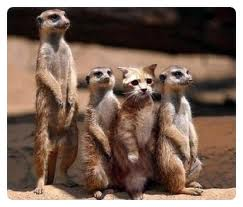
\includegraphics[width=0.48\textwidth]{./Figures/meerkat.jpg}
  \end{center}
  \vspace{-20pt}
  \legend{\textsf{난 누군가. 그리고 여긴 또 어딘가.}}
  \vspace{-10pt}
\end{figure}
한 가지 당부하자면, 질문하는 것을 겁내지 마라. 질문 좀 했다고 해서 선배들이
혼내거나, 이 아이는 왜 이리 멍청한 것일까라고 한탄하거나 하는 일은
없다. (...아마도?) 오히려 이 아이는 선배에게 먼저 다가와주는 귀여운 아이구나라며
이쁨 받을 확률이 더 높다. 모르는 것은 부끄러운 것이 아니다. 오히려 소위
쪽팔릴까봐 모르는 것을 물어보지 못하는 것이야 말로 부끄러운 행동이다.  연구에 막
입문한 사람들이기에, 조금 더 풀어서 써보면, 질문을 많이 하라는 것은 연구를
시작하는데 있어서도 마찬가지이다. 처음 교수님과 면담하거나 팀 미팅에 들어 가보면
신입생 중 십중팔구는 '이게 대체 무슨 소리지?, 나는 누구인가, 그리고 또 여긴
어딘가' 라며 공황상태에 빠지게 될 것인데, 그건 당연한 거다.
\vspace{\baselineskip}

교수님과 대학원생은, 그 분야에 대해서 짧게는 수 학기, 길게는 수 년을 판
사람인데, 이제 갓 연구를 시작한 새내기가 그 사람들 간의 대화를 100\% 이해하는
것이 가당키나 한 일이라고 보는가? 그런 경험은 당신만 겪는 일이 아니니,
의기소침해지거나, 더 나아가 '난 학부 때 너무 놀았나봐 난 글러먹었어'라며 겁먹은
타조마냥 땅에 머리 콕 처박고 자학모드에 들어가거나 하지 않았으면 한다. 그렇게
고뇌와 번민 속에서 허우적거릴 기력과 시간이 있으면 당장 교수님이나 선배를
찾아가서 질문하는 것이 백배천배 낫다. 교수님과 선배님이 신입생 골려주기 위해
어려운 용어를 쓰는 것이 아니다. 단지, 그 사람들은 당신이 못 알아듣는 것을 모르고
평소와 같이 말하고 있었을 뿐이다. 당신이 못 알아듣는 점에 대해 질문하면 당신이
아직 연구 궤도에 올라오지 못한 신입생이란 것을 그제서야 깨닫고 친절히 지금 무슨
이야기를 하고 있는 것인지 풀어서 설명해주실 것이다.  \vspace{\baselineskip}

기초적인 것도 모르는 것 같아서 질문하기에 너무 부끄러워 나중 그냥 따로 찾아보거나
공부하겠다고? 우리 솔직해지자. 그간 중고등학교와 대학교를 합쳐 근 10년 공부했으면
자기 자신에 대해서 좀 알 때가 되지 않았는가. 그 분야를 스스로 찾아서 공부하겠다고?
설령 당신이 칭찬할만한 의지력의 소유자여서 공부하려 하는 시도는 했다고
치자. 교수님들과 선배님들의 이야기는, 연구의 최전선에 있는, 따끈따끈한 것들이
많을텐데, 그 정보가 어디 있는지 어떻게 알 것이며, 어디서 찾을 것인가? 책?
네이버? 위키피디아? 답은 논문이다. 자 그러면, ADS나 arXiv 가서 논문 하나 출력해서
읽어보아라. 아마 abstract, introduction 채 읽기도 전에 논문을 활활 불태우고 싶은
충동에 휩싸일 것이다.  \vspace{\baselineskip}

물론 연구자라면 언젠가는 의무적으로 혼자서 자료를 찾고 모르는 것을 고민하면서
각자의 연구를 개척하며 걸어가는 순간이 오게 된다. 하지만 스스로 일어나 걸을 수
있게 되기까지, 부모님께서 지켜보는 가운데 숱하게 넘어지고 도움 받는 과정이 있다는
것을 잊어서는 안 된다. 대학원 석사 과정으로 입학한다는 건, 연구 인생으로 보면
걸음마를 떼기 시작하는 단계다. 아기가 스스로 걷지 못한다고 그걸 탓하는 사람은
없고, 또 걷지 못한다는 사실에 자괴감에 빠지는 아기는 없다. 대학원 첫 학기는
무엇을 질문해도 다 용서되는 특권을 가진, 연구 인생에서 다시는 오지 않을 가장
소중한 시간이다. 그 소중한 시간을 부디 낭비하지 말고 알차게 사용하길 바란다.
\vspace{\baselineskip}

단, 질문을 할 때, 몇 가지 에티켓 정도는 지키도록 하자.
\begin{enumerate}
\item 자기가 할 수 있는 선에서는 스스로 최선을 다해서 시도해보자. (그렇다고 앞
  문단을 깡그리 잊고, 혼자 이해할 수 없는 분야에 독학한다고 매진하지는 말고...)
  예를 들어, 당신이 처음 리눅스를 접하면 아무것도 모를 것이고 접속하고 계정
  만드는 것까지 선배의 도움을 받아야할 것이다. 하지만, 어느 정도 리눅스를 다룰 수
  있게 된 이후에도 '폴더는 어떻게 만들어요?' '폴더는 어떻게 지워요?' '이거 왜
  복사가 안될까요?' 등, 인터넷 검색만 해봐도 주르륵 뜨는 수준의 질문을 계속하는
  것도 예의 있는 행동은 아니다.
\item 질문은 최대한 구체적으로 하자. 물론, 아무런 지식 기반이 없으면, 자기가 뭘
  모르는지도 확실히 모를 수도 있다는 것은 이해하지만, 두루뭉실한 질문은 선배가
  들었을 때 친절히 답변해주고 싶어도 '어쩌라고?'라는 생각이 들기 마련이다.  예를
  들어 밑도 끝도 없이 '측광 어떻게 해요?' 라고 물어보면 선배는 그저 '잘' 이라고
  밖에 대답해줄 수밖에 없다. 그렇기에 '선생님께서 어떤어떤 일을 저에게 시키려고
  하는 것 같습니다. 그런데 홈페이지 갔는데 자료를 어떻게 받는지 잘
  모르겠네요. 그리고 측광하는 건 어떤 프로그램을 써야하는가요?' 라고 질문을
  구체적으로 하자.
\item 한 선배에게 집중질문 하지 말자. 앞서 질문 좀 했다고 뭐라하는 선배 없다고
  했지만, 어디까지나 '인간적인' 범위 내에서의 이야기지, 하루 종일 하나부터 열까지
  한 선배만 붙잡고 있다면, 그 선배도 사람인 이상 짜증이 날 수 밖에 없다.  (특별히
  자기에게 신경을 많이 써주는 선배분께는 감사하다고 캔커피 하나 정도 사드리는
  센스를 발휘하는 것도 좋다)
\end{enumerate}
\vspace{\baselineskip}

마지막으로, 사족을 덧붙이면 선배 및 동기와 친해지라는 것이다. 연구 생활 역시 사회
생활의 하나이고, 연구자들 간의 교류는 연구자의 중요한 덕목 중 하나이다. 실제로
선후배 동기들 간의 대화로부터 연구 내외적인 면에서 많은 조언 및 아이디어를
주고받을 수 있다. 자신은 백년에 한 번 나올까말까한 천재이기 때문에 천상천하
유아독존으로 살아가겠다는 신입생이 아니라면, 주위 사람들과 친목 다지는 것 역시
소홀히 하지 말고, 그러기 위한 노력의 일환으로 학과 행사에 적극적으로
참석하라. 연례 학과 행사는 Chapter 2에서 상세하게 다루었다. 그 행사들 중 더
중요하고 덜 중요한 행사가 어디있겠냐만, 특히 신입생들은 공식적으로 자기 소개를
앞에 나가 하게 되는 행사 (1학기라면 신년 교례회 및 개강파티/탁구대회/등산,
2학기라면 MT/등산) 및, 비공식적으로 매학기 초에 열리는 개강파티에는 반드시
참석한다는 마음을 갖도록 하자.  \vspace{\baselineskip} 리 생각보다 양이
많아지기는 했지만, 완벽한 안내서라고 하기에는 미흡한 점이 많이 있다. 각 분야에서
좀 더 자세히 언급했어야하는 내용들이 생략된 부분들도 있고, 특히 연구 방법에서
사용되는 다양한 도구들에 대해서는 각 도구들마다, 이 안내서만큼이나 길게
설명했어야하는 부분들이 있음에도 다 생략하였다. 이러한 자세한 설명들은 전문
서적이나 몇몇 대학원생들이 기획하고 있는 다른 안내서를 참고하기를
바란다. 더불어, 인터넷 대학원생 게시판 (\url{http://astro.snu.ac.kr/~grad})을
통해 대학원생들 사이의 노하우를 공유하는 장이 마련되어있으니, 이를 적극
활용하도록 하자.  \vspace{\baselineskip}

더불어, 시간이 지남에 따라 이 안내서에 담겨있는 내용들, 특히 행정적인 사항들, 은
변동 사항이 있을 수 있다. 안내서 편집부는 매년 개정된 사항들을 담아 안내서를 수정
보완할 계획이긴 하지만, 편집부를 너무 믿지는 말자. 우리도 사람이고, 귀차니즘에
시달릴 가능성이 높다.  \vspace{\baselineskip}

'마지막으로' 라고 말하고 훈화를 끝낼 줄을 모르는 교장 선생님처럼 마무리 멘트가
길어졌다. 이 글을 읽게 된 여러분의 앞에 펼쳐질 천문학이라는 바다 위의 항해는
때로는 잠잠한 바다에 순풍을 다는 항해가 될 것이고, 때로는 풍랑을 만나 표류하기도
할 것이며, 어쩌면 암초를 만나 좌초할 위기에 처할지도 모른다. 하지만 어느 순간에
있든 자기의 지금까지 항해를 되돌아 봤을 때, 스스로 만족할 수 있는 멋진 항해를
하기를 기원한다.
\begin{thebibliography}{9}
\bibitem{manual_ljh} 이준협 2006, \emph{서울대학교 천문학과 대학원에 진학하는 신입생들을 위한 안내서}. 링크: \url{http://astro.snu.ac.kr/~jhlee/bin/ez2000b/ezboard.cgi?db=kasi_pub&action=read&dbf=18&page=3&depth=1}
\bibitem{manual_jc} 천문학과 저널클럽 회원 일동 2011, \emph{천문학과 대학원생을 위한 저널클럽 (Ver 1.0)}. 링크: \url{http://astro1.snu.ac.kr/home/kor/journal/file/Introduction_JC_ver1.pdf}
\end{thebibliography}

\clearpage
\twocolindex
\pagestyle{index}

%\renewcommand{\chaptermark}[1]{}
\renewcommand{\preindexhook}{%
하고 싶은 말.\vskip\onelineskip}
\indexintoc

%%%\raggedright does nasty things to index entries
\printindex

\cleardoublepage \thispagestyle{empty} \null%\vfil
\vskip\onelineskip\vskip\onelineskip\vskip\onelineskip\vskip\onelineskip\vskip\onelineskip\vskip\onelineskip\vskip\onelineskip\vskip\onelineskip\vskip\onelineskip\vskip\onelineskip
\begin{adjustwidth}{0.5in}{0.5in}
\begin{center}
{\Large\textsf{만든이들}}
\end{center}
\begin{center}
\vskip\onelineskip
\textsf{1장: 김두호, 윤요셉, 이재형, 임형묵, 김용정 \\\vskip\onelineskip
2장: 서우영, 강월랑, 김예솔, 박근홍, 박다우, Dr. 박홍수, 신재진, 이헌철 \\\vskip\onelineskip
3장: 장인성, 고유경, 김용범, 박대성, 오세명, 홍주은 \\\vskip\onelineskip
4장: 박근홍, 김두호, 장인성, 현민희, 곽한나 \\\vskip\onelineskip
편집부: 손주비, 김정규}\\
\vskip\onelineskip
\textsf{Special Thanks to: Prof. 박용선, Prof. 이명균, Dr. 김창구}

\vskip\onelineskip\vskip\onelineskip\vskip\onelineskip
{\footnotesize{이 문서는 LaTeX에서 memoir 클래스, kotex 패키지 등을 이용해 만들어졌습니다.}}\\
\vskip\onelineskip
{\footnotesize{책값은 공짜입니다. (고마우신 분들은 개별적인 사례를 ...)}}
\vskip\onelineskip
{\footnotesize{잘못된 책은 못 바꾸어 드립니다. (미안합니다...)}}
\end{center}
\end{adjustwidth}

\end{backmatter}

\end{document}